
\typeout{new file: New_Species_RadCal_Chapter.tex}

\chapter{The New Fuel Species in RadCal}
\label{chap:new_species}

The original RadCal data have been supplemented with new tabulated experimental data for the following fuels: Ethylene ($\rm C_2H_4$), Ethane ($\rm C_2H_6$), Propylene ($\rm C_3H_6$), Propane ($\rm C_3H_8$), Toluene ($\rm C_7H_8$), \textit{n}-Heptane ($\rm C_7H_{16}$), Methanol ($\rm CH_3OH$), Methyl Methacrylate ($\rm C_5H_8O_2$). These new data have been obtained through Wakatsuki Fourier Transform Infra-Red (FTIR) measurements for wavenumbers between 700--4000~cm$\rm ^{-1}$. See Ref.~\cite{Wakatsuki2005b} for a detailed description of the experimental methodology.

The sections below briefly describe the molecules and their IR active molecular bands. Bands bounds used in RadCal are tabulated with a brief description of the band assignment and their integrated band intensity (see definition below) at the lowest temperature is also included. Unlike the data previously included in RadCal that contained a mix of tabulated and modeled data, the species data presented here in the chapter are all tabulated.

\section{Integrated band intensity}
\label{sec:integrated_intensity}

A useful quantity to compare the relative importance of the different IR bands is provided by the integrated band intensity, $\alpha_i$, defined for the $i$th participating species as:
\be\label{eq:alpha}
  \alpha_i(T) = \displaystyle\int_{\om_{\min}}^{\om_{\max}} \bar{\kappa}_i(\om',T) \; \d \om'
\ee
whose units are $\rm {atm^{-1} cm^{-2}}$. The integrated band intensity is an intrinsic property of a molecule directly related to its geometry, its elements, and the nature of the chemical bonds. It is proportional to the amplitude of the electric moment variations for a vibration-rotation transition \cite{Matheson1932}. It is usually referred to as the coefficient $C_1$ in the exponential wide-band model.

The value of the spectral absorption coefficient, $\bar{\kappa}_i$, is averaged over a narrow band whose spectral width, $\Delta \om$, varies from 5~cm$^{-1}$ for $\om < $ 1100~cm$^{-1}$, to 25~cm$^{-1}$ for 1100~cm$^{-1} \leq \om < $ 5000~cm$^{\rm -1}$, and to 50~cm$^{\rm -1}$ for 5000~cm$^{\rm -1}\leq \om$. In the sections below, value were obtained by integrated the narrow band absorption coefficients over the band of interest.

\section{Fitting procedure}

In Section~\ref{Sec::SNBM}, expressions for the Elsasser, Goody, and Malkmus narrow band models were presented, see Eqs.~\ref{eq::Elsasser}, \ref{eq::Goody}, and \ref{eq::Malkmus}. Each gives a functional expression of the spectral transmissivity over narrow bands in the form:
\be
 \bar{\tau}_{\omega} = f(\bar{\kappa}_{\omega},\beta_{\omega},U),
\ee
where the expression of $f$ depends on the model chosen; the pressure-path $U =  P_i L$ is known from the experimental configuration; the experimental spectral transmissivity $\bar{\tau}_{\omega}$ is obtained by FTIR measurements; and the couple $\bar{\kappa}_{\omega},\beta_{\omega}$ are the sought parameters. In the following, the subscript $_\omega$ denoting the spectral dependence of the quantities is omitted for ease of reading.

To find the optimal narrow band model parameters for each model, at a given temperature and at a given wavenumber, a fitting objective function was minimized using a least-square fitting approach. The objective function $\mathcal{F}$ was defined as:
\be
 \mathcal{F}_i = \dfrac{|\bar{\tau}_{exp,i}-f(\bar{\kappa},\beta,U_i)|}{\bar{\tau}_{exp,i}},
\ee
where the subscript $_{exp}$ denotes experimentally measured values, and $_i$ denotes an experimental condition of  pressure-path. The experimental transmissivity relative to the $i^{th}$ pressure-path is denoted $\bar{\tau}_{exp,i}$. This is an averaged value over the narrow band interval at the desired resolution. Typically three different pressure-paths were used for each temperature and fuel. The narrow band parameters $\left(\bar{\kappa},\beta\right)$ hence found minimize the square of the \textit{l}$\rm ^2$-norm of the objective function $\mathcal{F}$:
\be
 \min\limits_{\left(\bar{\kappa},\beta\right)}\|\mathcal{F}\|_2^2 = \min\limits_{\left(\bar{\kappa},\beta\right)}\left(\displaystyle\sum \limits_i \left(\dfrac{\bar{\tau}_{exp,i}-f(\bar{\kappa},\beta,U_i)}{\bar{\tau}_{exp,i}}\right)^2\right).
\ee

The spectral narrow band parameters were obtained for all the fuels presented in this section, for the three aforementioned narrow band models. As a verification test, the experimental transmissivities obtained were reconstructed using the narrow band models and compared with the measured values. For each experimental condition, very good agreements were observed between the synthetic and the experimental transmissivity profiles regardless of the narrow band model. No model stands out nor performs better than the other two.

The similar accuracy of three different narrow band models is likely a result of the small number of pressure-paths used to fit the data;  the fitted narrow-band parameters were obtained by fitting only three experimental pressure-paths. In previous works, the appropriate band narrow band model was selected based on the value of the model deviation from the experimental data, see Ref.~\cite{Kunitomo1975}. This is an valid method as long as the experimental data has lower error than that associated with any narrow band models. Here, the experimental error associated with the mean absorption coefficient is 5\% \cite{Wakatsuki2008}, which is higher than the difference between experimental and synthetic data for each model.

It is customary to validate the choice of the assumed narrow band model or to derive its parameters from the knowledge of the integrated band intensities, $\alpha$, defined by Eq.~\ref{eq:alpha}. Experimentally, $\alpha$ is computed from the extrapolation technique first proposed by Wilson and Wells \cite{Wilson1946,Thorndike1947} and further explained in Penner~\cite{Penner1959}. The technique is briefly recalled. A parameter $B$ is defined as:
\be
 B = \dfrac{1}{P_iL} \displaystyle\int\limits_{band} -\ln(\tau_{\omega}) {\rm d} \omega.
\ee
The apparent integrated band intensity, $\mathcal{A}$, defined as:
\be
 \mathcal{A} = \displaystyle\int\limits_{band}{-\ln{\tau_{\omega}}} {\rm d} \omega
\ee
relates with $B$ through the relation:
\be
\label{eq:LineofGrowth}
\mathcal{A} = P_iL B.
\ee
The work by Wilson and Wells \cite{Wilson1946,Thorndike1947} showed that the $\alpha$ relates with the parameter $B$ through:
\be
\label{eq:Exp_alpha}
 \alpha = \lim\limits_{P_iL\rightarrow 0} B
\ee

Hence, the experimental value for $\alpha$ can be obtained through extrapolation of $A$ to the origin and
measuring the slope at the origin. While a direct extrapolation is not recommended as it may be subject to significant error as mentioned by Kaplan \textit{et al.}, \cite{Kaplan1956a}, a extrapolation using an educated curve-of-growth procedure \cite{Kaplan1956a} can help alleviate this problem. The functional relation between the absorption and the pressure-path can be assumed to be a function of the unknown $\alpha$ and some characteristic line width. Fitting the experimental data is required to obtain the unknown parameters and it provides a more rigorous evaluation of $\alpha$.

While a representative functional relation can be derived for a fundamental band, \textit{i.e.} a band associated with only one vibration transition mode, it is more difficult to do so for bands that are the results of multiple vibration modes. This is the case for all the species presented here. Hence, no extrapolation was performed as they could lead to bias depending on the extrapolation method used. Instead, following comments presented in Modest~\cite{Modest2013}, the Malkmus model was chosen as it is recognized as the best for polyatomic molecules. Verification tests for each species are presented in Section~\ref{sec:verification}. Some of the data, ethane, ethylene, and propane, have been carefully examined and some species were compared with the HITRAN 2012 edition. See Lecoustre \textit{et al.} \cite{Lecoustre2014} for more details.

\clearpage

\section{Ethylene: $\rm C_2H_4$}

\subsection{Integrated Band Intensity}

Ethylene, $\rm C_2H_4$, is a plane symmetrical molecule and belongs to the point group $D_{2h}$. It has 12 vibrational modes. In RadCal, its IR spectrum is divided into four distinct bands that are associated with different vibrational modes, see Table \ref{Table::C2H4}. The bands from 750 - 1250~cm$^{-1}$ and 1300 - 1600~cm$^{-1}$ are associated with the bending motion of the $\rm CH_2$ groups. The band between 1750 and 2075~cm$^{-1}$ is associated with the stretching motion of the carbon double bond, $\rm C=C$. The fourth band from 2800 - 3400~cm$^{-1}$ is associated with the stretching of the CH groups. The strongest absorption band is located at lower wavenumbers, between 780 and 1250~cm$^{-1}$. This indicates the propensity of ethylene to strong participation to the radiative heat exchange corresponding to low to moderate temperatures. This spectral range corresponds to the highest blackbody spectral emittance at temperatures ranging between 400 to 700~K which are characteristic of cooler regions of the fuel rich cores for liquid and solid fires.
\begin{table}[ht]
    \centering
    \caption{Spectral bands of $\rm C_2H_4$ included in RadCal.}
    \vspace{0.1in}
    \label{Table::C2H4}
    \begin{tabular}{|c|c|c|c|c|}
      \hline
      Band \# & \multicolumn{2}{|l|}{Bounds (cm$\rm ^{-1}$) } & Assignment & $\alpha(T=296 \; {\rm K}) \; (\rm {atm^{-1} cm^{-2}})$\\
      \cline{1-5}
      1 & 750  & 1250 &  $\rm CH_2$ Bend      & 371 \\
      2 & 1300 & 1600 &  $\rm CH_2$ Bend      & 42  \\
      3 & 1750 & 2075 &  $\rm C=C$  Stretch   & 20  \\
      4 & 2800 & 3400 &  $\rm C-H$  Stretch   & 198 \\
      \hline
    \end{tabular}
\end{table}
Band~1 is the strongest absorbing band. All the ethylene IR spectral absorption data were obtained from high resolution FTIR experiments with temperatures varying from 296~K to 1000~K. See Wakatsuki \cite{Wakatsuki2005b} for more details about the experimental process followed to obtain the experimental data.

\subsection{Malkmus Narrow Band Parameters}

The spectral absorption coefficients were obtained by least square fitting of the experimental transmissivity using the Malkmus model. The ethylene narrow band parameters, $\bar{\kappa}$ and $\beta$, for temperatures ranging from 296~K to 1000~K are plotted in Figures~\ref{fig:ethylene_kappa_beta1}--\ref{fig:ethylene_kappa_beta4} for Bands 1 to 4.

\newpage

\begin{figure}[p]
\begin{center}
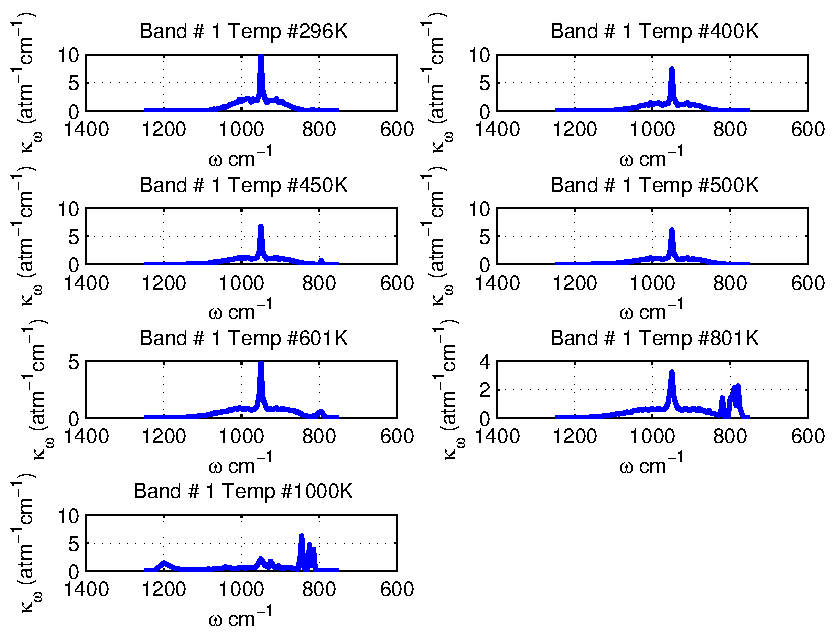
\includegraphics[width=5.0in]{Figures/Ethylene_Kappa_Band1_MALKMUS.pdf}
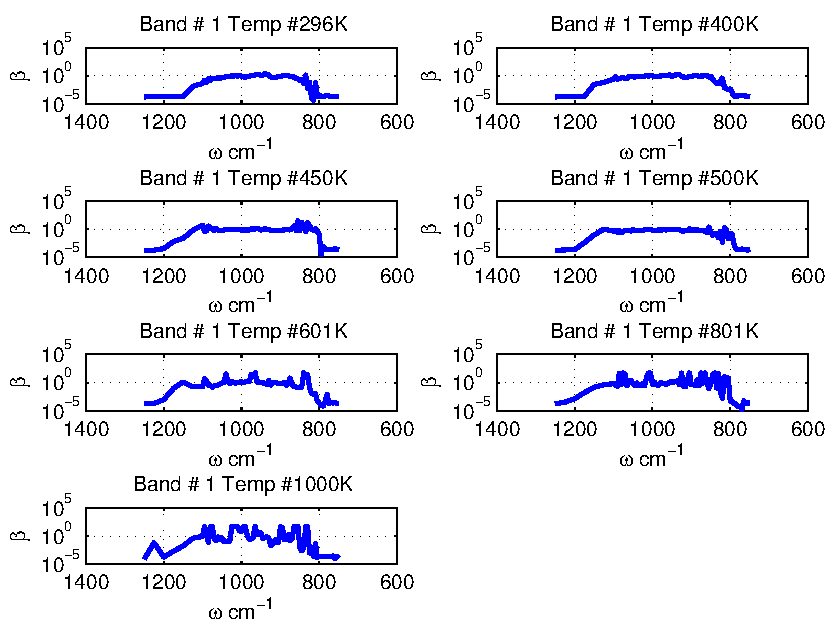
\includegraphics[width=5.0in]{Figures/Ethylene_Beta_Band1_MALKMUS.pdf}
\end{center}
\caption{Ethylene narrow band parameters $\bar{\kappa}$ and $\beta$ obtained for the 750--1250~cm$^{-1}$ band corresponding to the bending motion of the $\rm CH_2$ chemical group. Temperatures plotted are: 296, 400, 450, 500, 601, 801, and 1000~K. The narrow band resolution $\Delta \om$ is 5~cm$^{-1}$.\label{fig:ethylene_kappa_beta1}}
\end{figure}

\begin{figure}[p]
\begin{center}
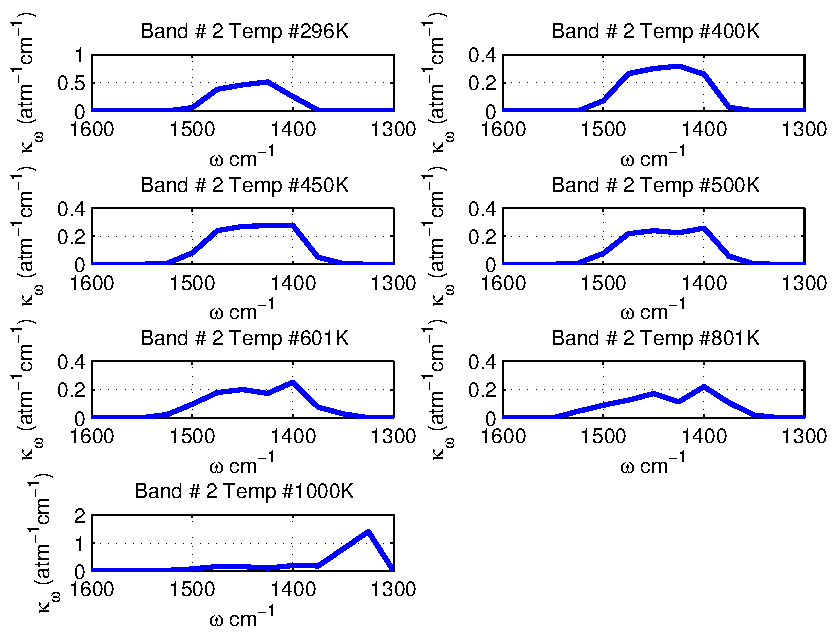
\includegraphics[width=5.0in]{Figures/Ethylene_Kappa_Band2_MALKMUS.pdf}
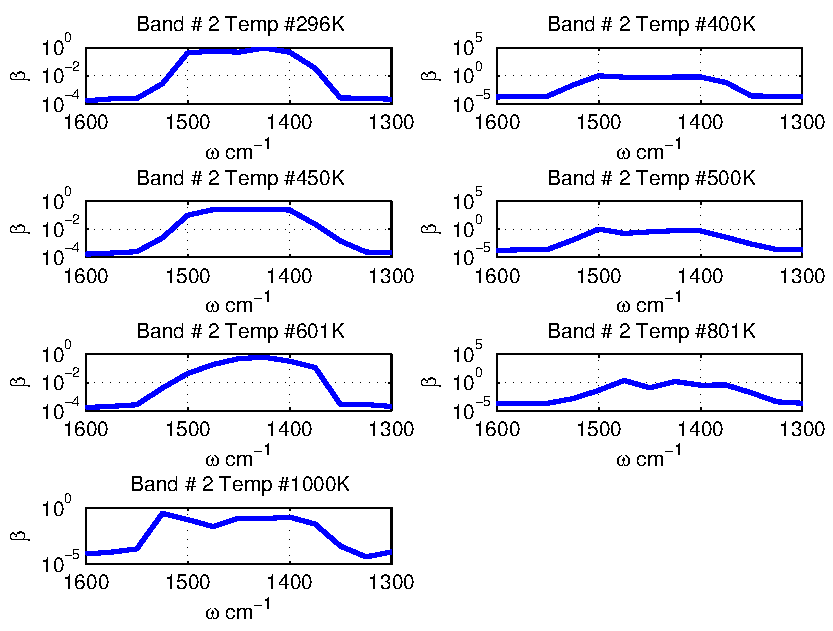
\includegraphics[width=5.0in]{Figures/Ethylene_Beta_Band2_MALKMUS.pdf}
\end{center}
\caption{Ethylene narrow band parameters $\bar{\kappa}$ and $\beta$ obtained for the 1300--1600~cm$^{-1}$ band corresponding to the bending motion of the $\rm CH_2$ chemical group. Temperatures plotted are: 296, 400, 450, 500, 601, 801, and 1000~K. The narrow band resolution $\Delta \om$ is 25~cm$^{-1}$.\label{fig:ethylene_kappa_beta2}}
\end{figure}

\begin{figure}[p]
\begin{center}
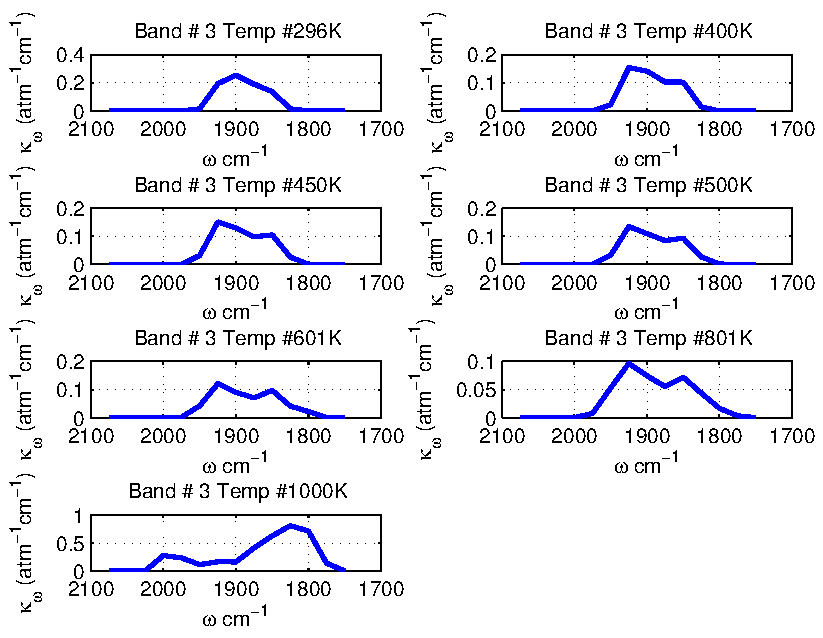
\includegraphics[width=5.0in]{Figures/Ethylene_Kappa_Band3_MALKMUS.pdf}
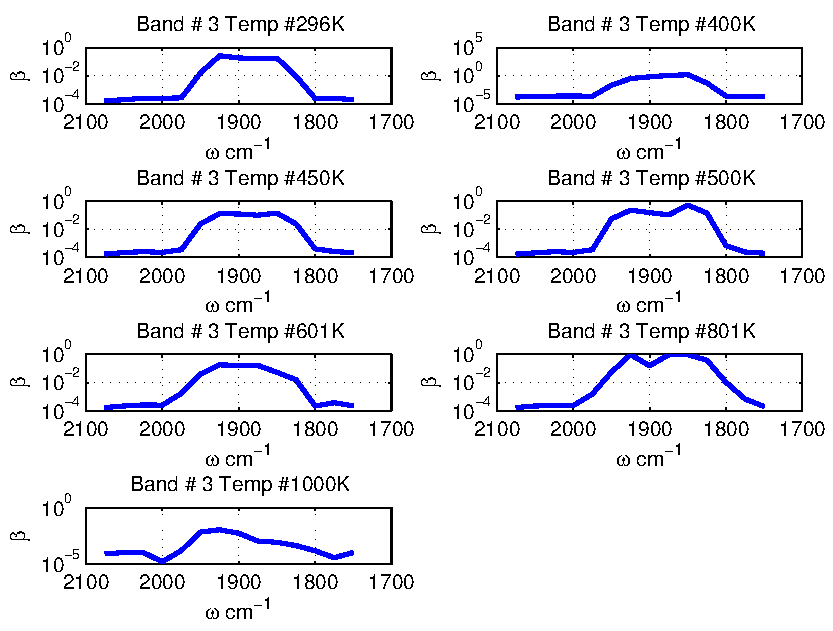
\includegraphics[width=5.0in]{Figures/Ethylene_Beta_Band3_MALKMUS.pdf}
\end{center}
\caption{Ethylene narrow band parameters $\bar{\kappa}$ and $\beta$ obtained for the 1750--2075~cm$^{-1}$ band corresponding to the stretching motion of the $\rm C=C$ chemical group. Temperatures plotted are: 296, 400, 450, 500, 601, 801, and 1000~K. The narrow band resolution $\Delta \om$ is 25~cm$^{-1}$.\label{fig:ethylene_kappa_beta3}}
\end{figure}

\begin{figure}[p]
\begin{center}
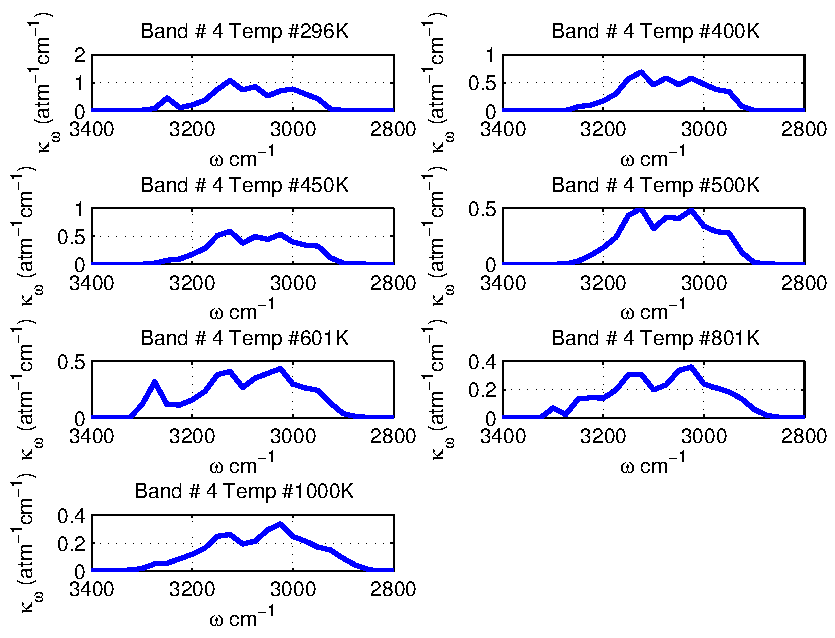
\includegraphics[width=5.0in]{Figures/Ethylene_Kappa_Band4_MALKMUS.pdf}
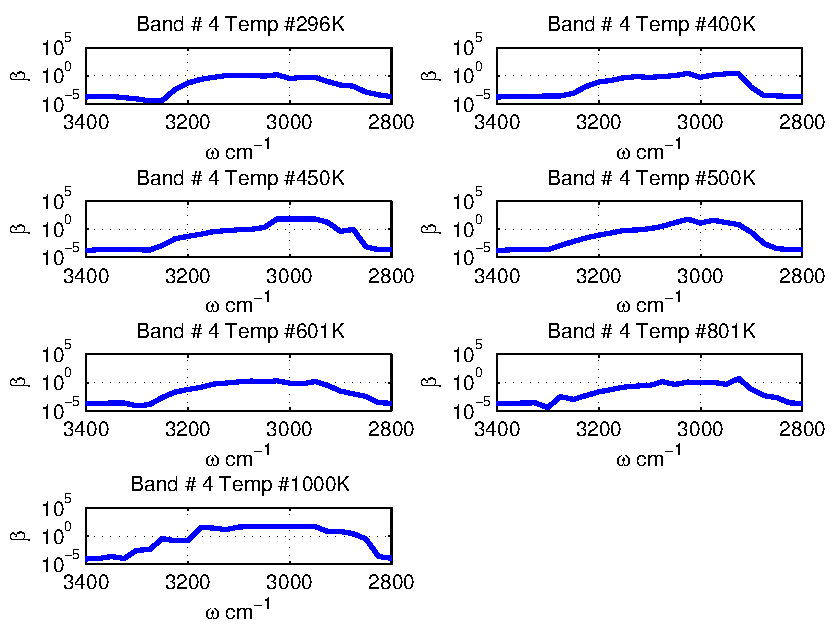
\includegraphics[width=5.0in]{Figures/Ethylene_Beta_Band4_MALKMUS.pdf}
\end{center}
\caption{Ethylene narrow band parameters $\bar{\kappa}$ and $\beta$ obtained for the 2800--3400~cm$^{-1}$ band corresponding to the stretching motion of the $\rm C-H$ chemical group. Temperatures plotted are: 296, 400, 450, 500, 601, 801, and 1000~K. The narrow band resolution $\Delta \om$ is 25~cm$^{-1}$.\label{fig:ethylene_kappa_beta4}}
\end{figure}

\FloatBarrier

\subsection{Verification SNB Parameters}

To assess the accuracy of the narrow band parameters $\bar{\kappa}$ and $\beta$, synthetic transmissivities were constructed for the same experimental conditions as the FTIR data and compare with it. This subsection plots the comparison and the relative error in transmissivity (relative to FTIR measurements) using the ethylene parameters presented in Figs.~\ref{fig:ethylene_kappa_beta1} to \ref{fig:ethylene_kappa_beta4}.


\begin{figure}[!h]
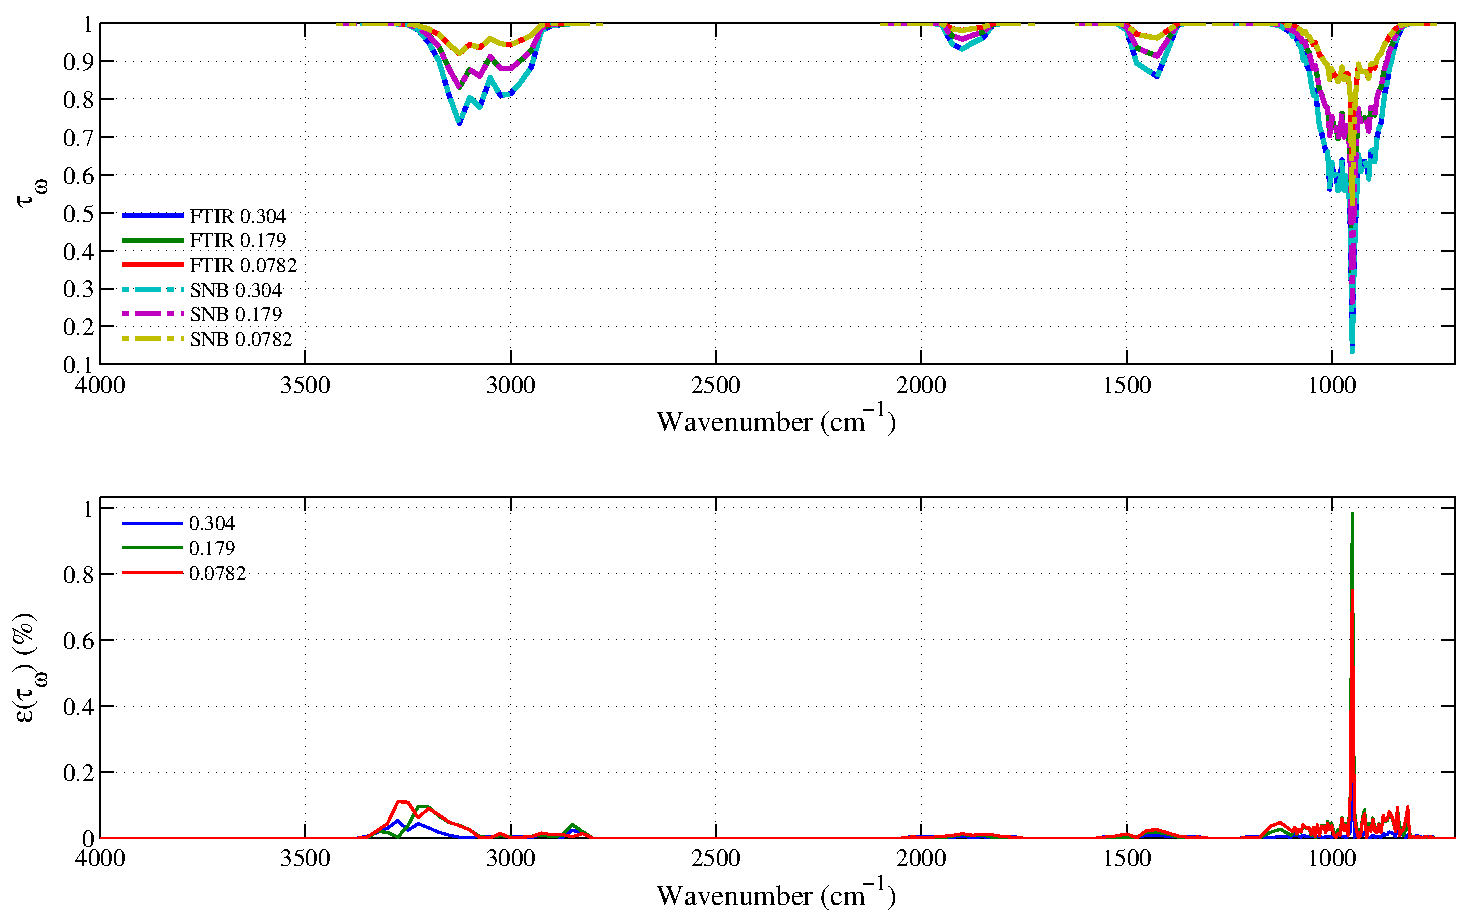
\includegraphics[width=\textwidth]{Figures/Comparison_Fit_Ethylene_MALKMUS_Temp296K.pdf}
\caption{Top: comparison between the experimental (FTIR, in solid lines) and the synthetic (dashed lines) spectral transmissivity profiles, denoted $\tau_{\omega}$, of an isothermal homogeneous column of ethylene. The synthetic profiles was generated using the Malkmus narrow band parameters presented in Figs.~\ref{fig:ethylene_kappa_beta1} to \ref{fig:ethylene_kappa_beta4}. Bottom: relative transmissivity error, denoted $\epsilon{(\tau_{\omega})}$, between the experiment and the synthetic profiles presented on the top figure. Three different pressure-paths are considered: 0.304, 0.179 and 0.0782 atm.cm. The gas temperature is set at 296~K and the total pressure is 101 kPa. Note: the experimental data resolution has been changed to match that of the narrow band model. \label{fig:ethylene_SNBVerify_296K}}
\end{figure}

\begin{figure}[p]
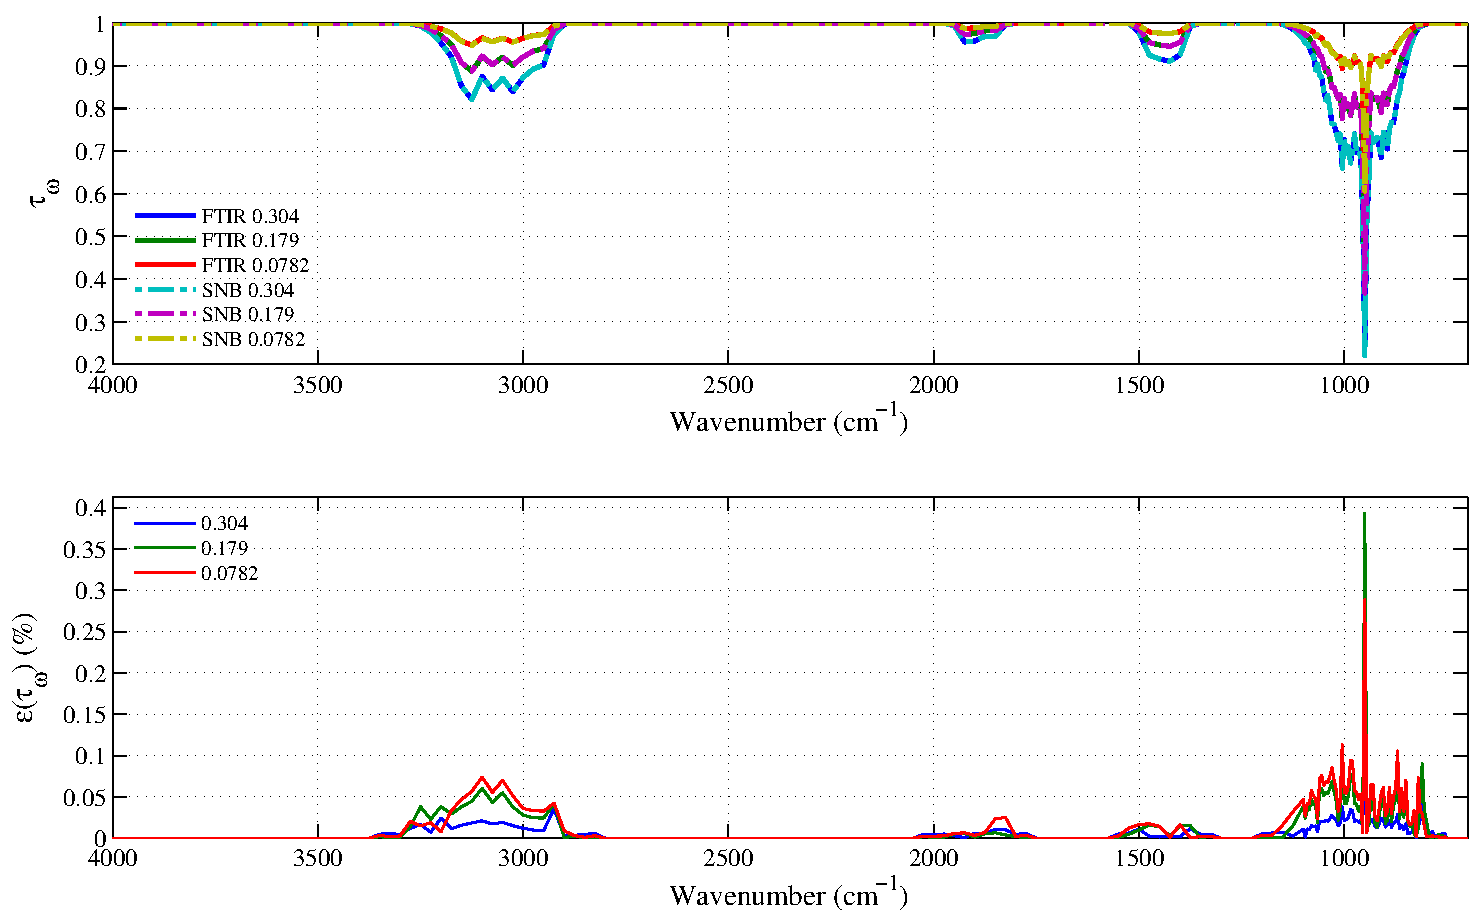
\includegraphics[width=\textwidth]{Figures/Comparison_Fit_Ethylene_MALKMUS_Temp400K.pdf}
\caption{Top: comparison between the experimental (FTIR, in solid lines) and the synthetic (dashed lines) spectral transmissivity profiles, denoted $\tau_{\omega}$, of an isothermal homogeneous column of ethylene. The synthetic profiles was generated using the Malkmus narrow band parameters presented in Figs.~\ref{fig:ethylene_kappa_beta1} to \ref{fig:ethylene_kappa_beta4}. Bottom: relative transmissivity error, denoted $\epsilon{(\tau_{\omega})}$, between the experiment and the synthetic profiles presented on the top figure. Three different pressure-paths are considered: 0.304, 0.179 and 0.0782 atm.cm. The gas temperature is set at 400~K and the total pressure is 101 kPa. Note: the experimental data resolution has been changed to match that of the narrow band model. \label{fig:ethylene_SNBVerify_400K}}
\end{figure}

\begin{figure}[p]
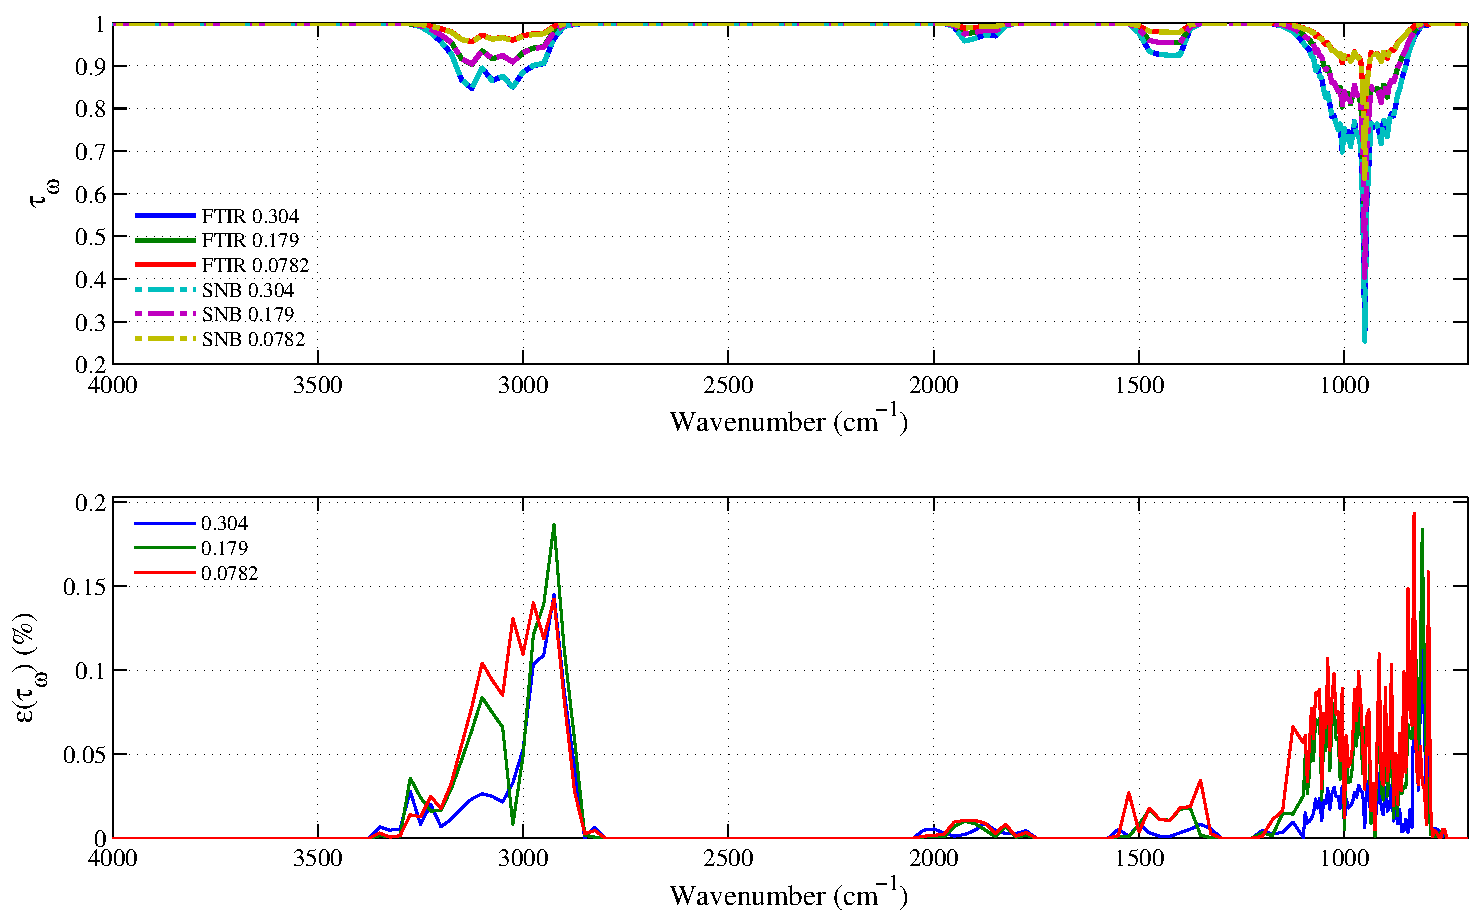
\includegraphics[width=\textwidth]{Figures/Comparison_Fit_Ethylene_MALKMUS_Temp450K.pdf}
\caption{Top: comparison between the experimental (FTIR, in solid lines) and the synthetic (dashed lines) spectral transmissivity profiles, denoted $\tau_{\omega}$, of an isothermal homogeneous column of ethylene. The synthetic profiles was generated using the Malkmus narrow band parameters presented in Figs.~\ref{fig:ethylene_kappa_beta1} to \ref{fig:ethylene_kappa_beta4}. Bottom: relative transmissivity error, denoted $\epsilon{(\tau_{\omega})}$, between the experiment and the synthetic profiles presented on the top figure. Three different pressure-paths are considered: 0.304, 0.179 and 0.0782 atm.cm. The gas temperature is set at 450~K and the total pressure is 101 kPa. Note: the experimental data resolution has been changed to match that of the narrow band model. \label{fig:ethylene_SNBVerify_450K}}
\end{figure}

\begin{figure}[p]
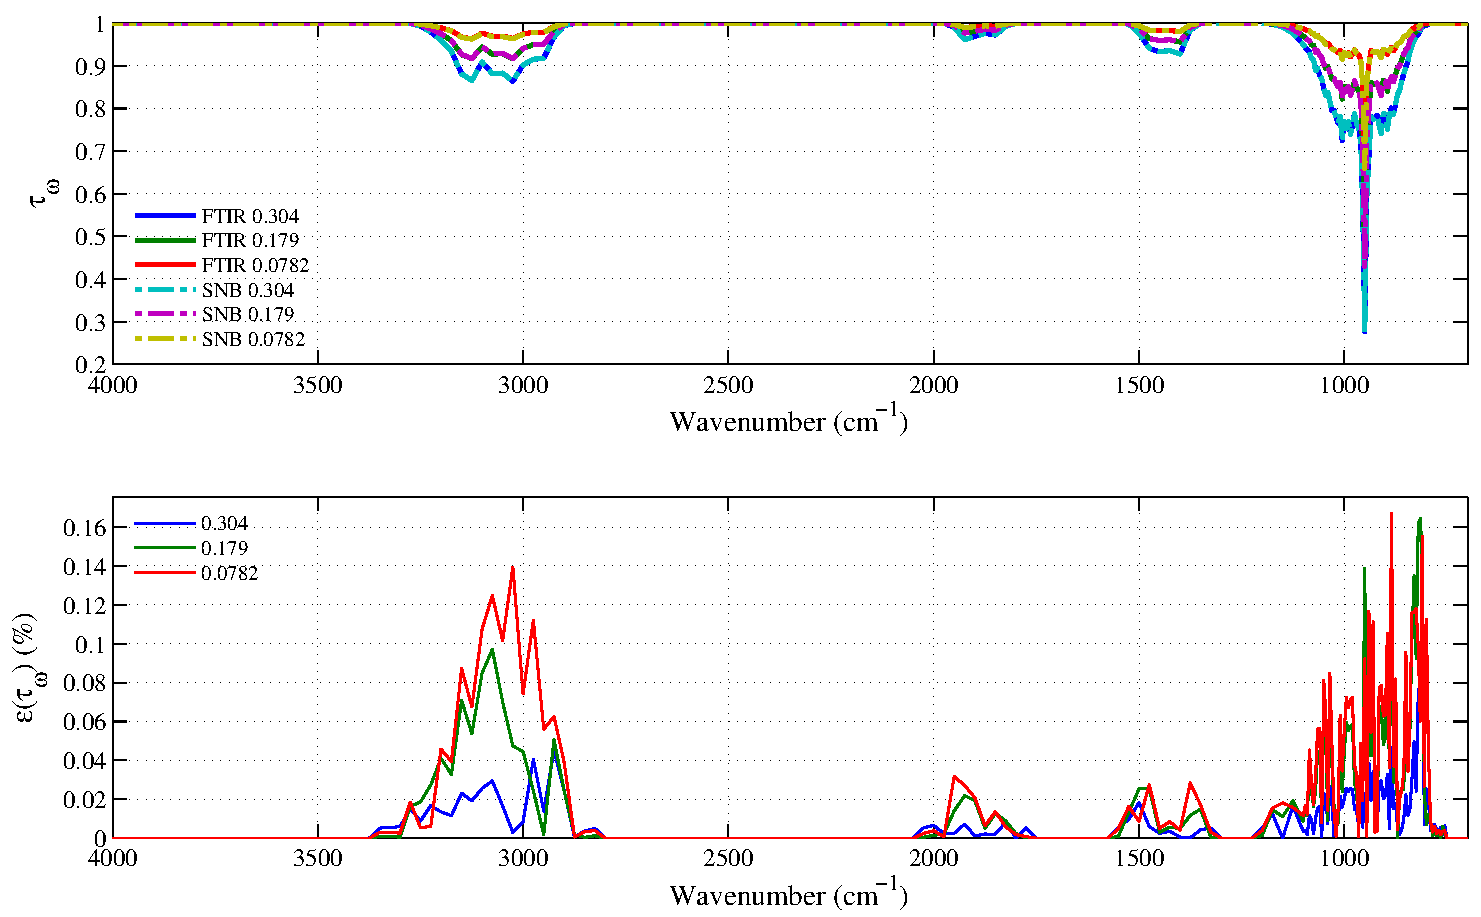
\includegraphics[width=\textwidth]{Figures/Comparison_Fit_Ethylene_MALKMUS_Temp500K.pdf}
\caption{Top: comparison between the experimental (FTIR, in solid lines) and the synthetic (dashed lines) spectral transmissivity profiles, denoted $\tau_{\omega}$, of an isothermal homogeneous column of ethylene. The synthetic profiles was generated using the Malkmus narrow band parameters presented in Figs.~\ref{fig:ethylene_kappa_beta1} to \ref{fig:ethylene_kappa_beta4}. Bottom: relative transmissivity error, denoted $\epsilon{(\tau_{\omega})}$, between the experiment and the synthetic profiles presented on the top figure. Three different pressure-paths are considered: 0.304, 0.179 and 0.0782 atm.cm. The gas temperature is set at 500~K and the total pressure is 101 kPa. Note: the experimental data resolution has been changed to match that of the narrow band model. \label{fig:ethylene_SNBVerify_500K}}
\end{figure}

\begin{figure}[p]
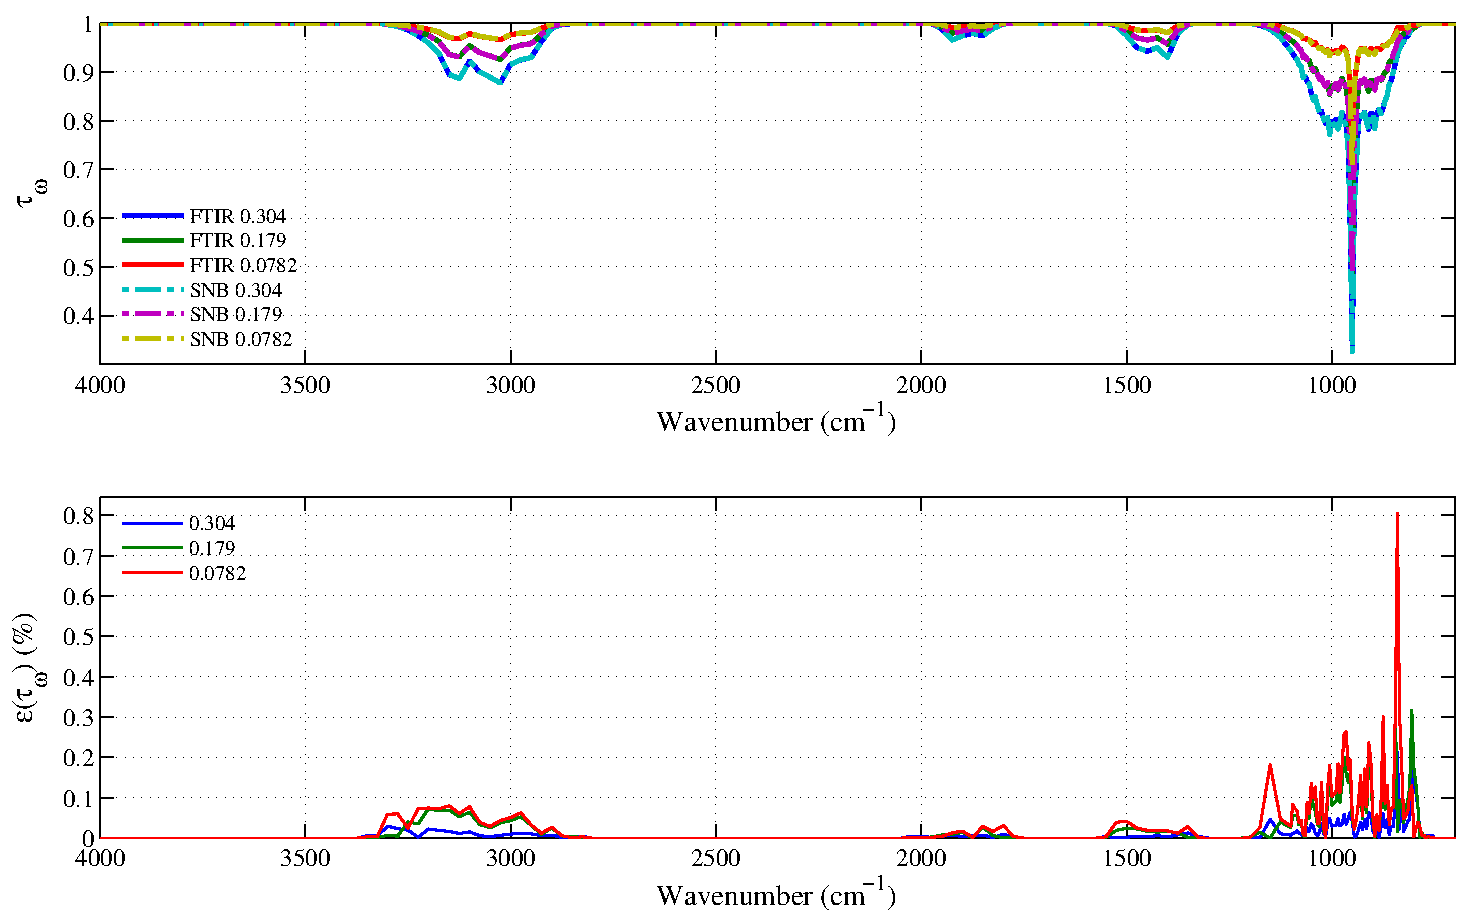
\includegraphics[width=\textwidth]{Figures/Comparison_Fit_Ethylene_MALKMUS_Temp601K.pdf}
\caption{Top: comparison between the experimental (FTIR, in solid lines) and the synthetic (dashed lines) spectral transmissivity profiles, denoted $\tau_{\omega}$, of an isothermal homogeneous column of ethylene. The synthetic profiles was generated using the Malkmus narrow band parameters presented in Figs.~\ref{fig:ethylene_kappa_beta1} to \ref{fig:ethylene_kappa_beta4}. Bottom: relative transmissivity error, denoted $\epsilon{(\tau_{\omega})}$, between the experiment and the synthetic profiles presented on the top figure. Three different pressure-paths are considered: 0.304, 0.179 and 0.0782 atm.cm. The gas temperature is set at 601~K and the total pressure is 101 kPa. Note: the experimental data resolution has been changed to match that of the narrow band model. \label{fig:ethylene_SNBVerify_601K}}
\end{figure}

\begin{figure}[p]
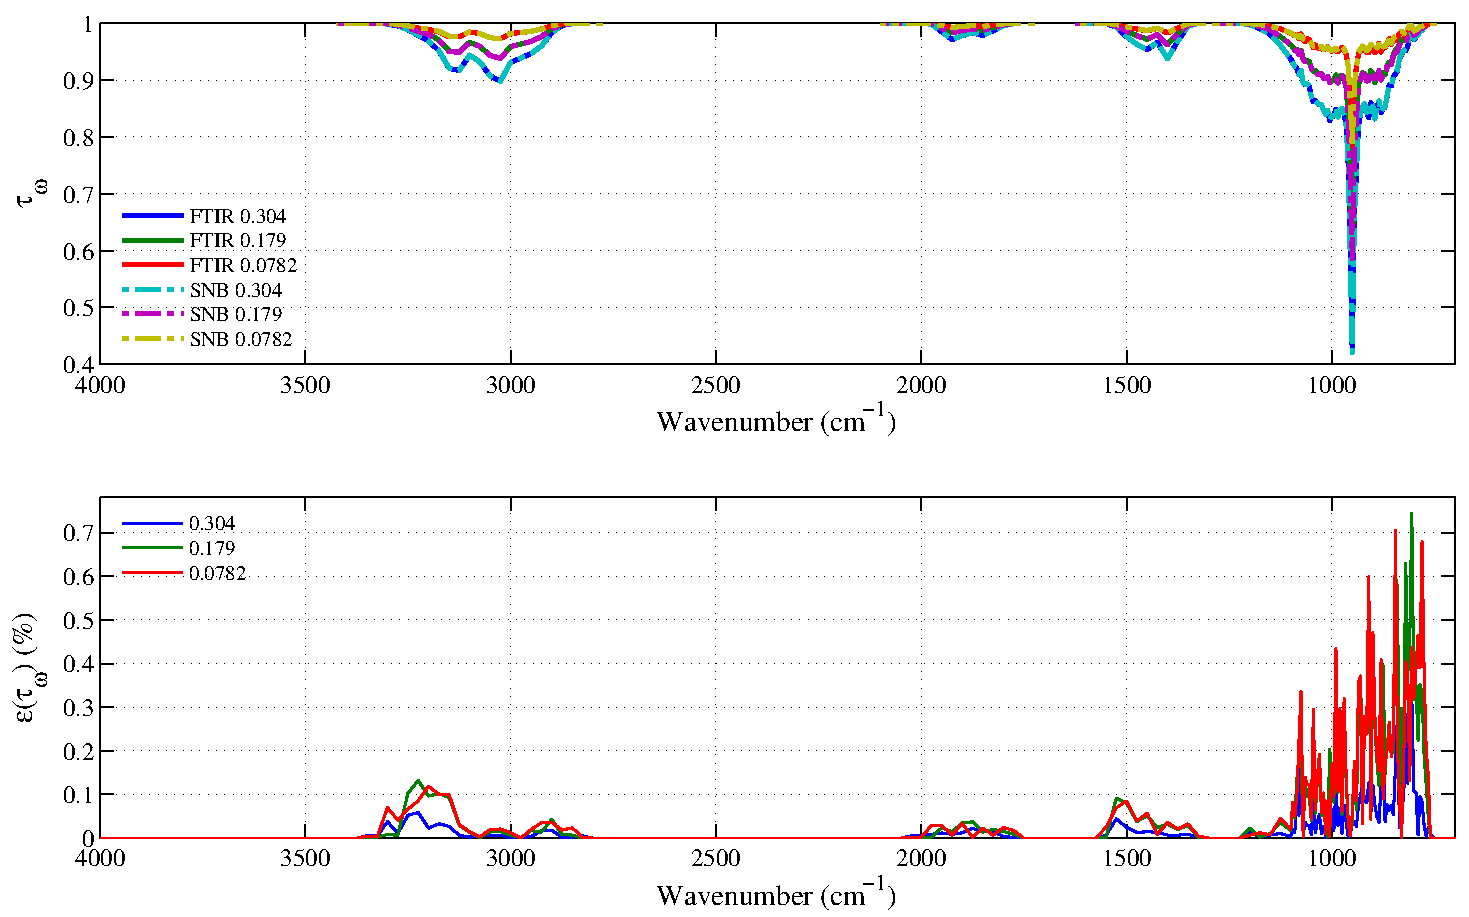
\includegraphics[width=\textwidth]{Figures/Comparison_Fit_Ethylene_MALKMUS_Temp801K.pdf}
\caption{Top: comparison between the experimental (FTIR, in solid lines) and the synthetic (dashed lines) spectral transmissivity profiles, denoted $\tau_{\omega}$, of an isothermal homogeneous column of ethylene. The synthetic profiles was generated using the Malkmus narrow band parameters presented in Figs.~\ref{fig:ethylene_kappa_beta1} to \ref{fig:ethylene_kappa_beta4}. Bottom: relative transmissivity error, denoted $\epsilon{(\tau_{\omega})}$, between the experiment and the synthetic profiles presented on the top figure. Three different pressure-paths are considered: 0.304, 0.179 and 0.0782 atm.cm. The gas temperature is set at 801~K and the total pressure is 101 kPa. Note: the experimental data resolution has been changed to match that of the narrow band model. \label{fig:ethylene_SNBVerify_801K}}
\end{figure}

\begin{figure}[p]
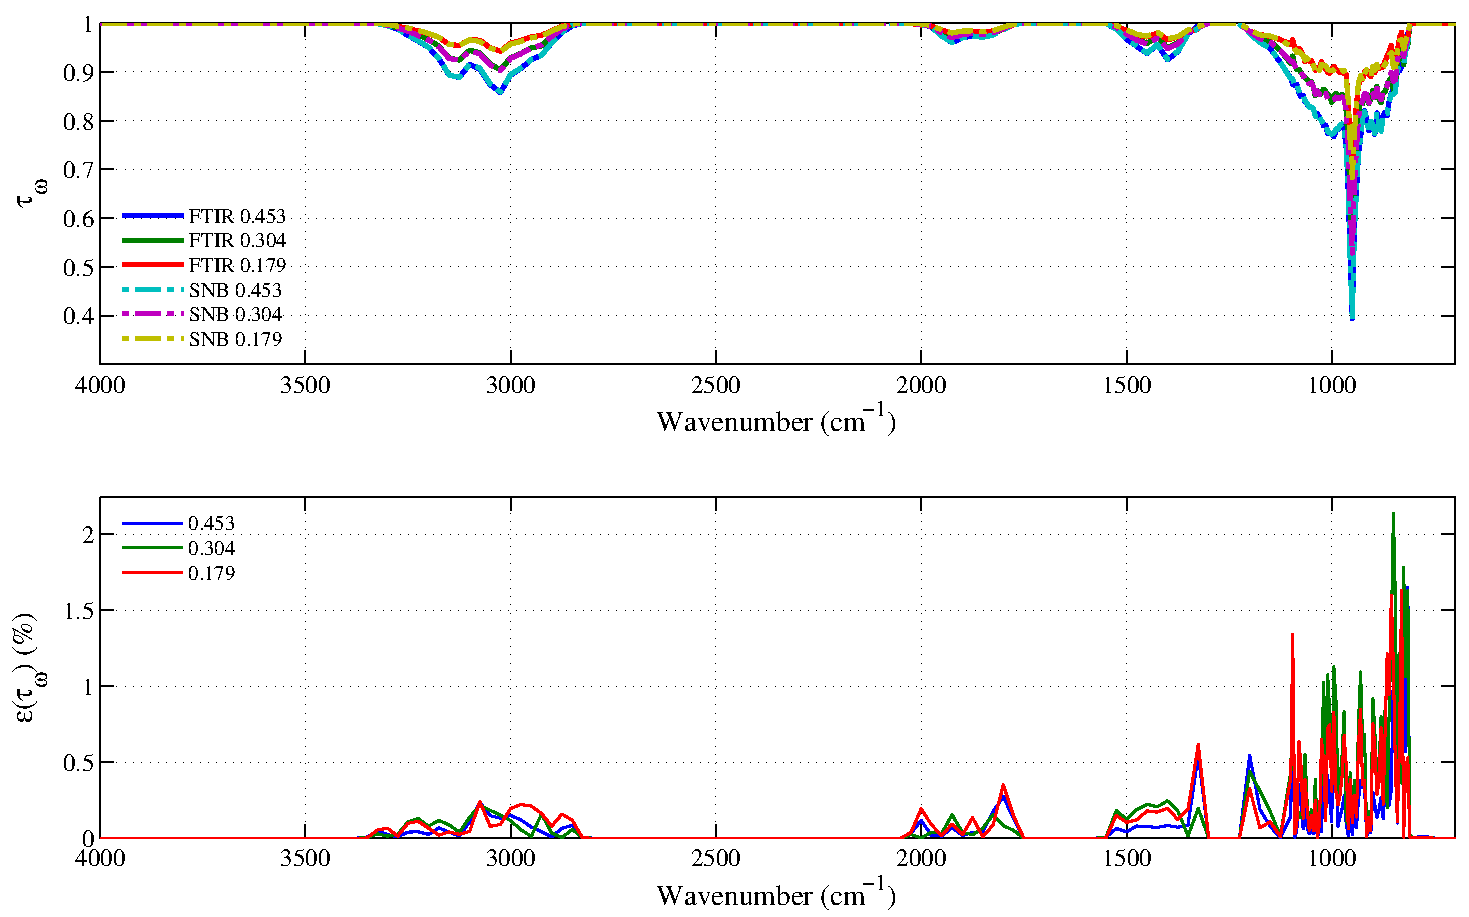
\includegraphics[width=\textwidth]{Figures/Comparison_Fit_Ethylene_MALKMUS_Temp1000K.pdf}
\caption{Top: comparison between the experimental (FTIR, in solid lines) and the synthetic (dashed lines) spectral transmissivity profiles, denoted $\tau_{\omega}$, of an isothermal homogeneous column of ethylene. The synthetic profiles was generated using the Malkmus narrow band parameters presented in Figs.~\ref{fig:ethylene_kappa_beta1} to \ref{fig:ethylene_kappa_beta4}. Bottom: relative transmissivity error, denoted $\epsilon{(\tau_{\omega})}$, between the experiment and the synthetic profiles presented on the top figure. Three different pressure-paths are considered: 0.304, 0.179 and 0.0782 atm.cm. The gas temperature is set at 1000~K and the total pressure is 101 kPa. Note: the experimental data resolution has been changed to match that of the narrow band model. \label{fig:ethylene_SNBVerify_1000K}}
\end{figure}


\clearpage

\section{Ethane: $\rm C_2H_6$}

\subsection{Integrated Band Intensity}

Ethane, $\rm C_2H_6$, has a three-fold axis of symmetry and belongs to the point group $D_{3d}$, \cite{Herzberg1949}. Being a non-linear molecule, it has 18 vibrational modes, but due to its symmetry, some modes are identical, and the number of distinct vibrational modes is reduced to 12. In RadCal, its spectra are defined by 3 distinct bands associated with different vibrational modes, see Table \ref{Table::C2H6}. The band from 730--1095~cm$^{-1}$ is associated with the rocking motion of the $\rm CH_3$ groups, the band from 1250--1700~cm$^{-1}$ is associated with the bending motion of the CH groups, and the main band between 2550--3375~cm$^{-1}$ is associated with the stretching of the CH groups.

The CH stretching band located from 2550--3375~cm$^{-1}$ has the lowest transmissivity, \textit{i.e.} highest absorption, and dominates absorption due to ethane for blackbody emissions at typical combustion temperatures between 1300~K and 1800~K, characteristic of sooting flames. At standard temperature and pressure, its integrated band intensity is more than 10 times the value of Band~2, and more than 20 times the value of Band~1.

\begin{table} [ht]
    \centering
    \caption{Spectral bands of $\rm C_2H_6$ included in RadCal.}
    \vspace{0.1in}
    \label{Table::C2H6}
    \begin{tabular}{|c|c|c|c|c|}
      \hline
      Band \# & \multicolumn{2}{|l|}{Bounds (cm$\rm ^{-1}$) } & Assignment & $\alpha(T=296 \; {\rm K}) \; (\rm {atm^{-1} cm^{-2}})$\\
      \cline{1-5}
      1 & 730  & 1095 &  $\rm CH_3$ Rock   &  30  \\
      2 & 1250 & 1700 &  $\rm CH$  Bend    &  64  \\
      3 & 2550 & 3375 &  $\rm CH$  Stretch &  774 \\
      \hline
    \end{tabular}
\end{table}

\subsection{Malkmus Narrow Band Parameters}

All the ethane IR spectral absorption data were obtained from high resolution FTIR experiments with temperatures varying from 296~K to 1000~K. The spectral absorption coefficients were obtained by fitting the experimental spectral transmissivity of a homogeneous column of isothermal ethane with a total pressure of 1~atm using the Malkmus model.

The ethane narrow band parameters, $\bar{\kappa}$ and $\beta$, for temperatures ranging from 296~K to 1000~K are plotted in Figures~\ref{fig:ethane_kappa_beta1}--\ref{fig:ethane_kappa_beta3} for Bands 1 to 3.

\newpage

\begin{figure}[p]
\begin{center}
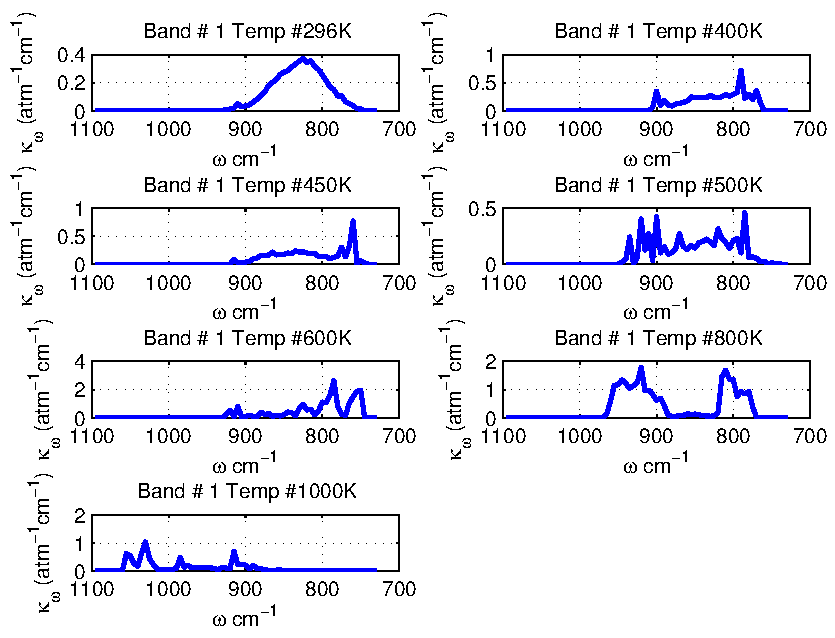
\includegraphics[width=5.0in]{Figures/Ethane_Kappa_Band1_MALKMUS.pdf}
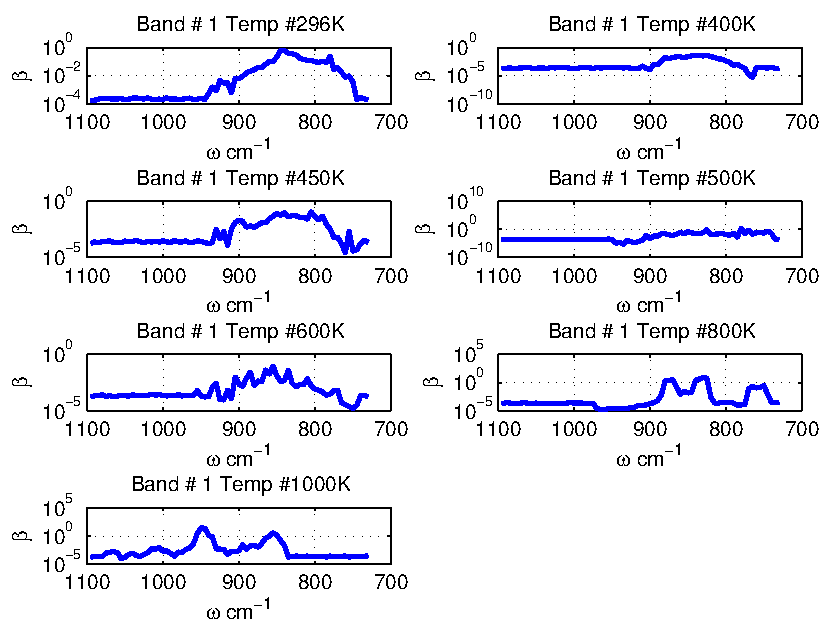
\includegraphics[width=5.0in]{Figures/Ethane_Beta_Band1_MALKMUS.pdf}
\end{center}
\caption{Ethane narrow band parameters $\bar{\kappa}$ and $\beta$ obtained for the 730--1095~cm$^{-1}$ band corresponding to the rocking motion of the $\rm CH_3$ chemical group. Temperatures plotted are: 296, 400, 450, 500, 600, 800, and 1000~K. The narrow band resolution $\Delta \om$ is 5~cm$^{-1}$.\label{fig:ethane_kappa_beta1}}
\end{figure}

\begin{figure}[p]
\begin{center}
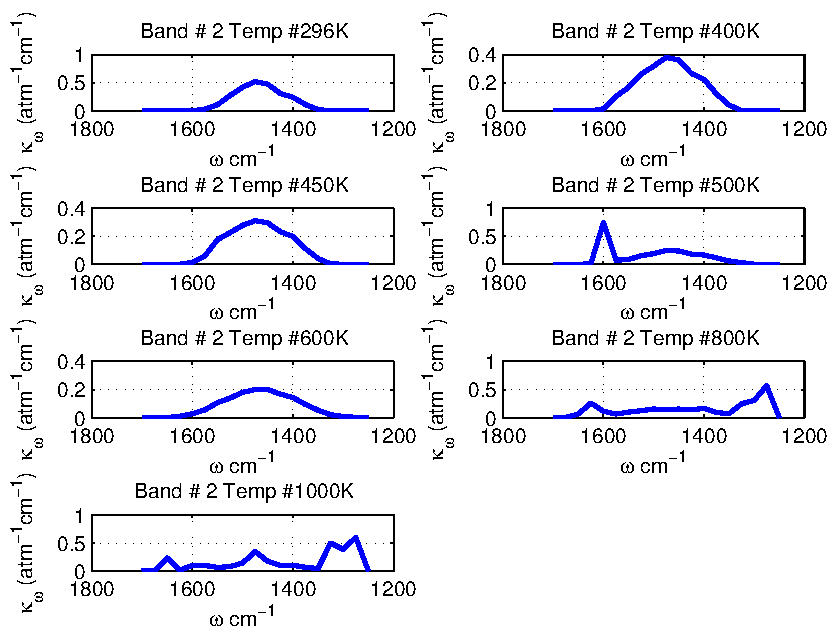
\includegraphics[width=5.0in]{Figures/Ethane_Kappa_Band2_MALKMUS.pdf}
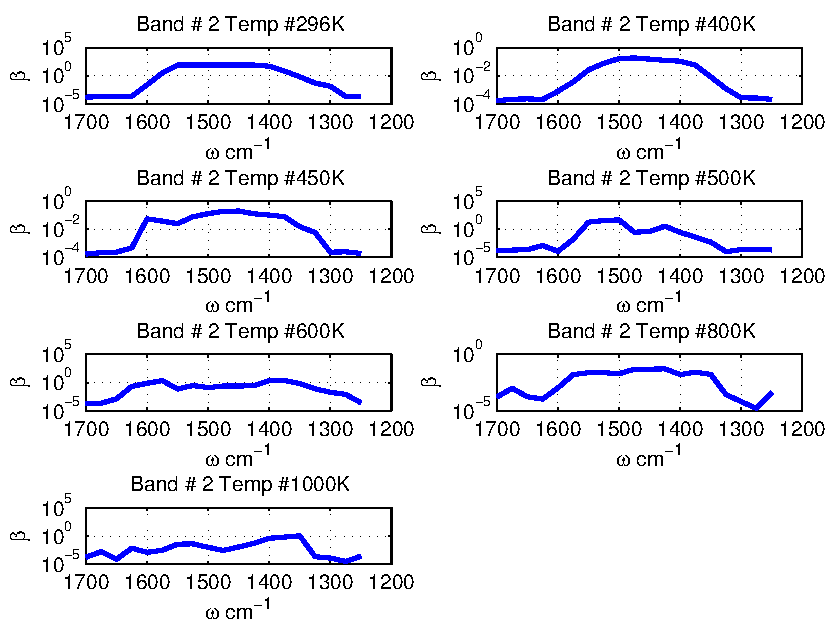
\includegraphics[width=5.0in]{Figures/Ethane_Beta_Band2_MALKMUS.pdf}
\end{center}
\caption{Ethane narrow band parameters $\bar{\kappa}$ and $\beta$ obtained for the 1250--1700~cm$^{-1}$ band corresponding to the bending motion of the $\rm CH$ chemical group. Temperatures plotted are: 296, 400, 450, 500, 600, 800, and 1000~K. The narrow band resolution $\Delta \om$ is 25~cm$^{-1}$.\label{fig:ethane_kappa_beta2}}
\end{figure}

\begin{figure}[p]
\begin{center}
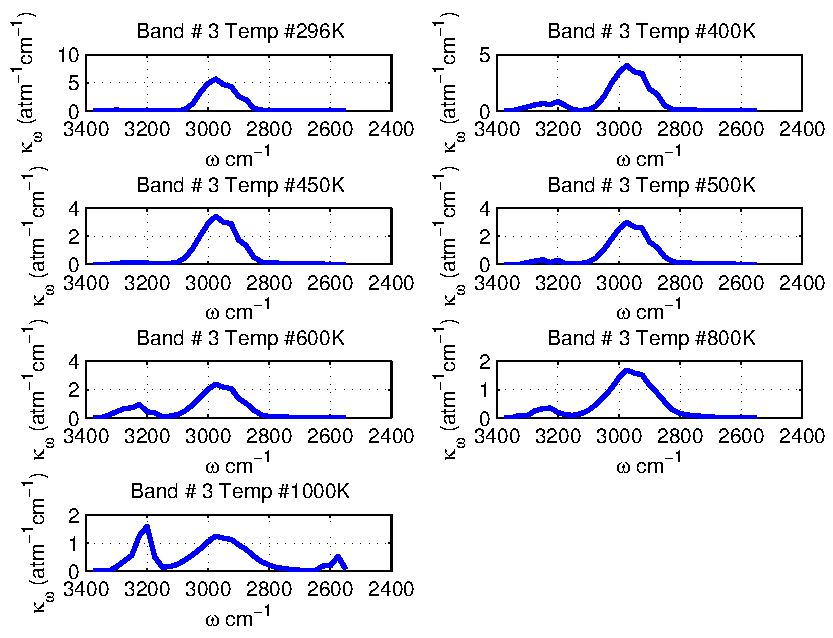
\includegraphics[width=5.0in]{Figures/Ethane_Kappa_Band3_MALKMUS.pdf}
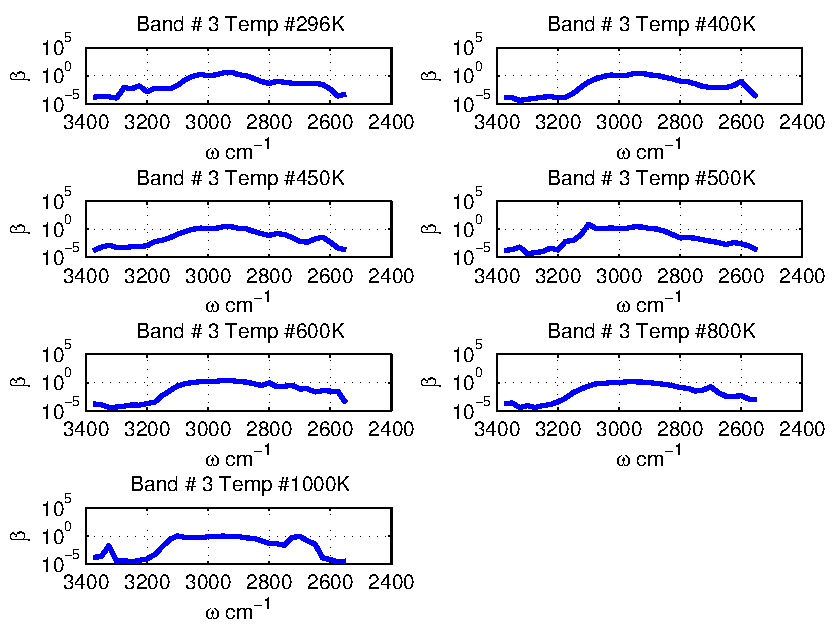
\includegraphics[width=5.0in]{Figures/Ethane_Beta_Band3_MALKMUS.pdf}
\end{center}
\caption{Ethane narrow band parameters $\bar{\kappa}$ and $\beta$ obtained for the 2550--3375~cm$^{-1}$ band corresponding to the stretching motion of the $\rm C-H$ chemical group. Temperatures plotted are: 296, 400, 450, 500, 600, 800, and 1000~K. The narrow band resolution $\Delta \om$ is 25~cm$^{-1}$.\label{fig:ethane_kappa_beta3}}
\end{figure}

\FloatBarrier

\subsection{Verification SNB Parameters}

To assess the accuracy of the narrow band parameters $\bar{\kappa}$ and $\beta$, synthetic transmissivities were constructed for the same experimental conditions as the FTIR data and compare with it. This subsection plots the comparison and the relative error in transmissivity (relative to FTIR measurements) using the ethane parameters presented in Figs.~\ref{fig:ethane_kappa_beta1} to \ref{fig:ethane_kappa_beta3}.

\begin{figure}[!h]
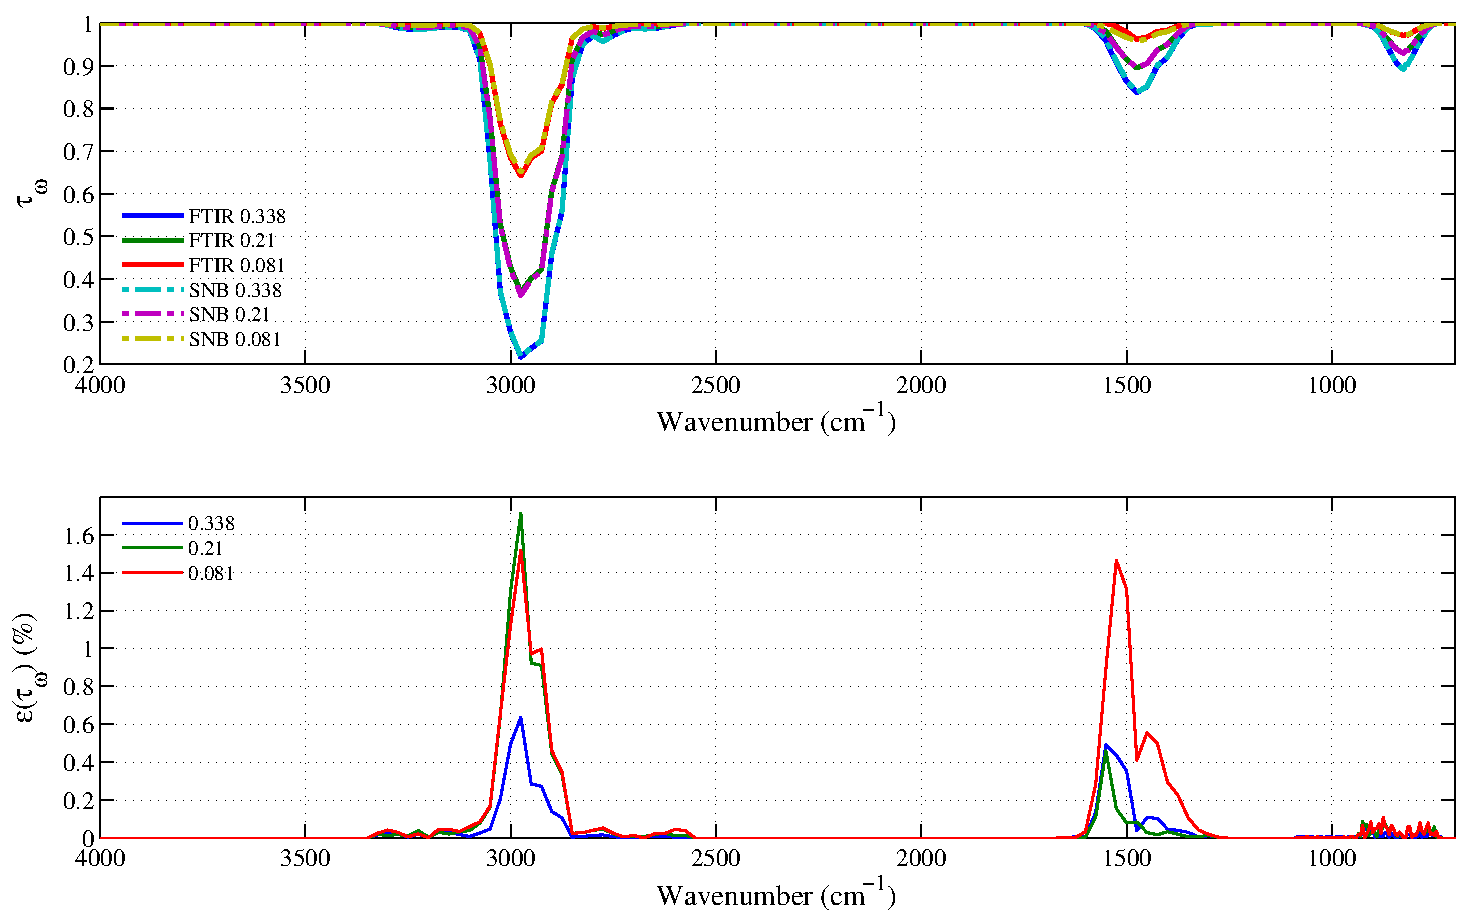
\includegraphics[width=\textwidth]{Figures/Comparison_Fit_Ethane_MALKMUS_Temp296K.pdf}
\caption{Top: comparison between the experimental (FTIR, in solid lines) and the synthetic (dashed lines) spectral transmissivity profiles, denoted $\tau_{\omega}$, of an isothermal homogeneous column of ethane. The synthetic profiles was generated using the Malkmus narrow band parameters presented in Figs.~\ref{fig:ethane_kappa_beta1} to \ref{fig:ethane_kappa_beta3}. Bottom: relative transmissivity error, denoted $\epsilon{(\tau_{\omega})}$, between the experiment and the synthetic profiles presented on the top figure. Three different pressure-paths are considered: 0.338, 0.21 and 0.081 atm.cm. The gas temperature is set at 296~K and the total pressure is 101 kPa. Note: the experimental data resolution has been changed to match that of the narrow band model. \label{fig:ethane_SNBVerify_296K}}
\end{figure}

\begin{figure}[p]
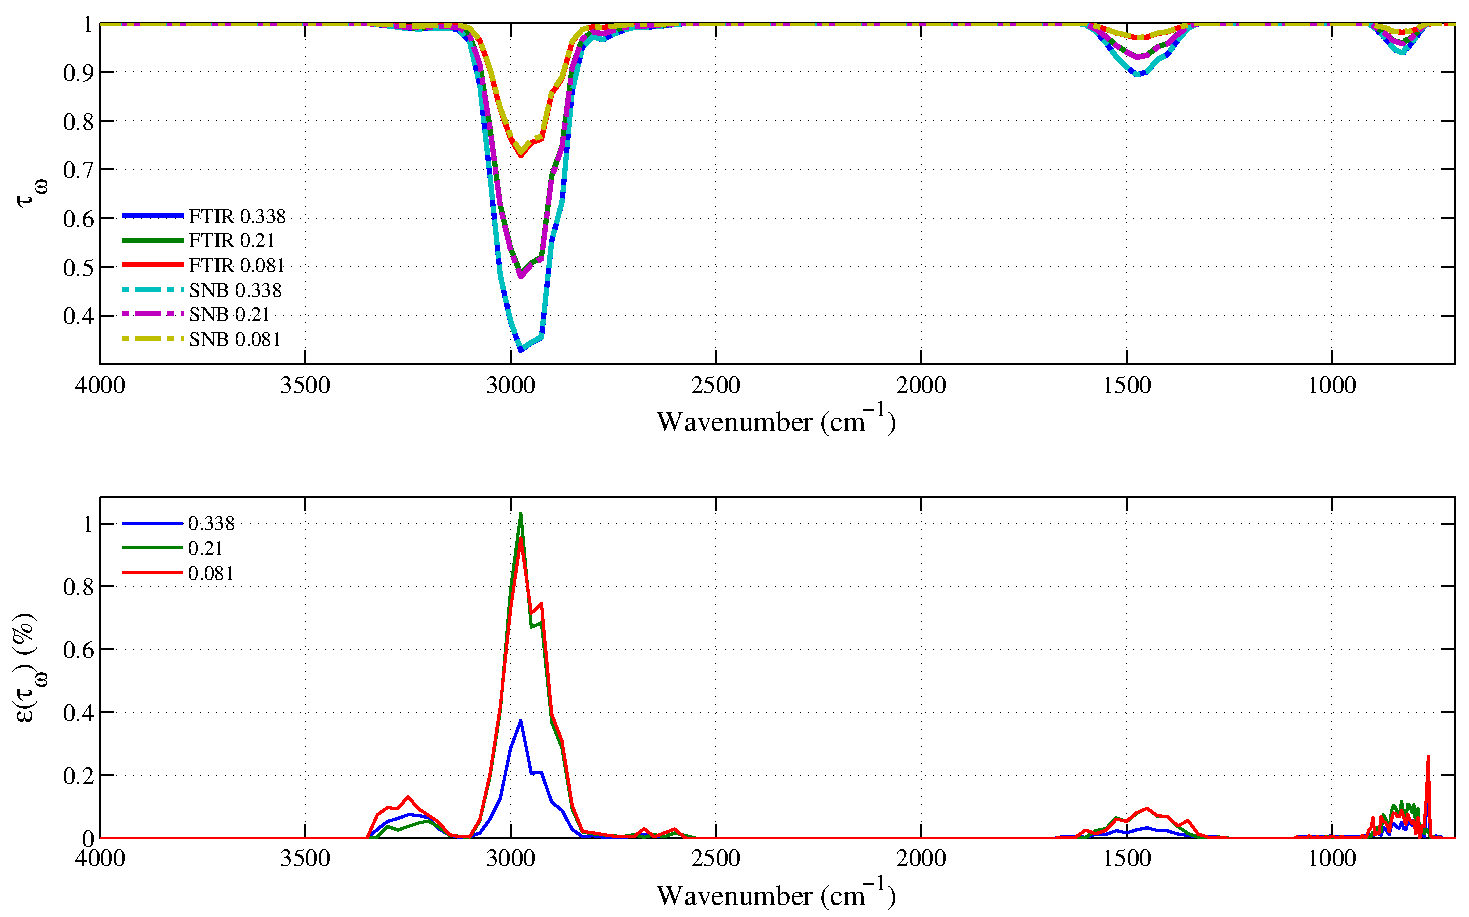
\includegraphics[width=\textwidth]{Figures/Comparison_Fit_Ethane_MALKMUS_Temp400K.pdf}
\caption{Top: comparison between the experimental (FTIR, in solid lines) and the synthetic (dashed lines) spectral transmissivity profiles, denoted $\tau_{\omega}$, of an isothermal homogeneous column of ethane. The synthetic profiles was generated using the Malkmus narrow band parameters presented in Figs.~\ref{fig:ethane_kappa_beta1} to \ref{fig:ethane_kappa_beta3}. Bottom: relative transmissivity error, denoted $\epsilon{(\tau_{\omega})}$, between the experiment and the synthetic profiles presented on the top figure. Three different pressure-paths are considered: 0.338, 0.21 and 0.081 atm.cm. The gas temperature is set at 400~K and the total pressure is 101 kPa. Note: the experimental data resolution has been changed to match that of the narrow band model. \label{fig:ethane_SNBVerify_400K}}
\end{figure}

\begin{figure}[p]
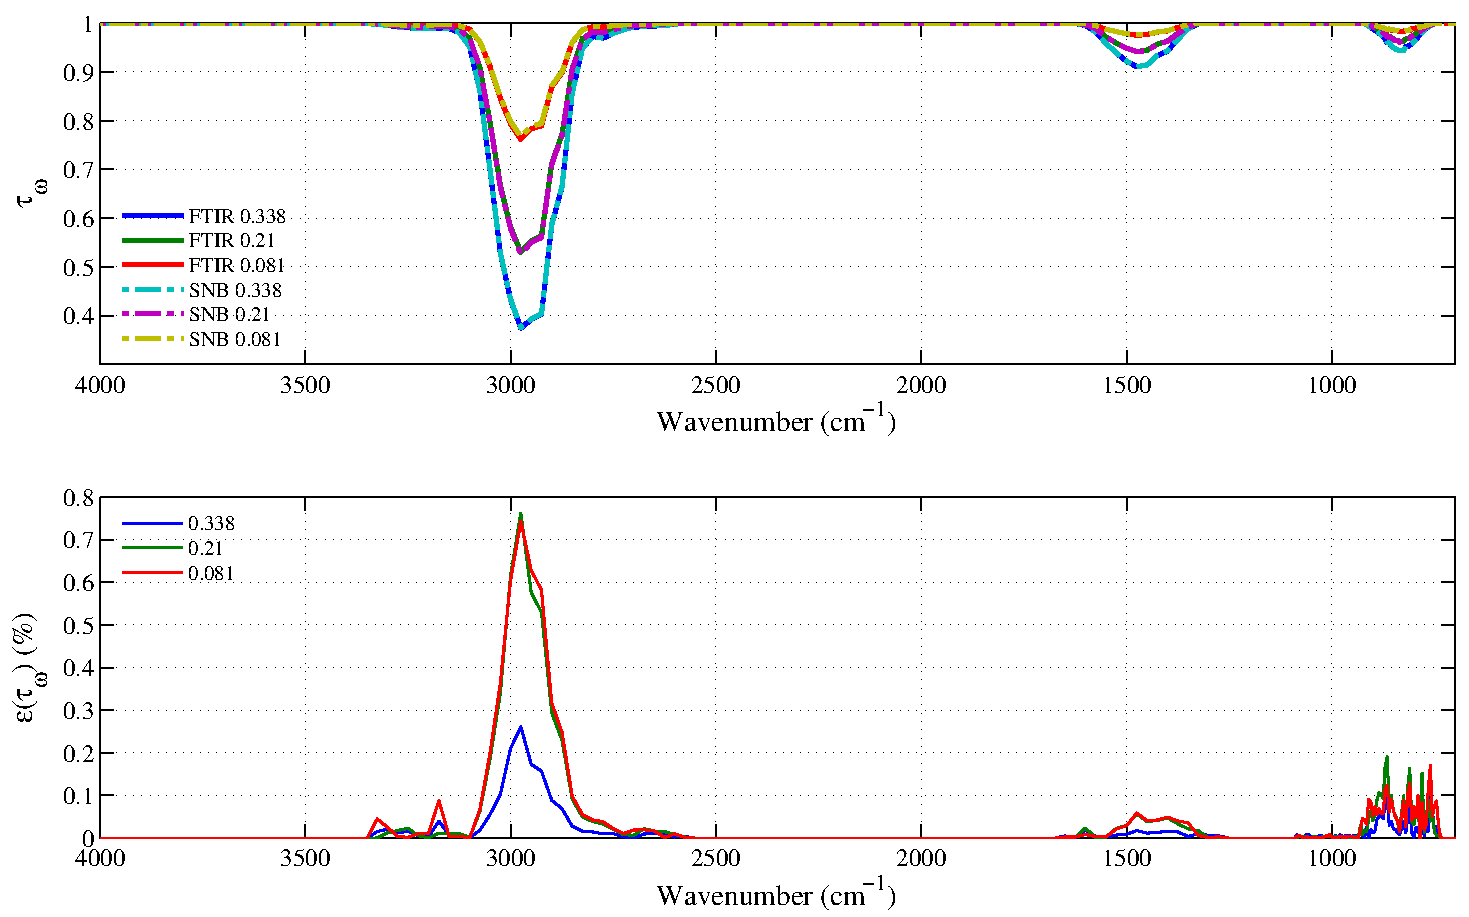
\includegraphics[width=\textwidth]{Figures/Comparison_Fit_Ethane_MALKMUS_Temp450K.pdf}
\caption{Top: comparison between the experimental (FTIR, in solid lines) and the synthetic (dashed lines) spectral transmissivity profiles, denoted $\tau_{\omega}$, of an isothermal homogeneous column of ethane. The synthetic profiles was generated using the Malkmus narrow band parameters presented in Figs.~\ref{fig:ethane_kappa_beta1} to \ref{fig:ethane_kappa_beta3}. Bottom: relative transmissivity error, denoted $\epsilon{(\tau_{\omega})}$, between the experiment and the synthetic profiles presented on the top figure. Three different pressure-paths are considered: 0.338, 0.21 and 0.081 atm.cm. The gas temperature is set at 450~K and the total pressure is 101 kPa. Note: the experimental data resolution has been changed to match that of the narrow band model. \label{fig:ethane_SNBVerify_450K}}
\end{figure}

\begin{figure}[p]
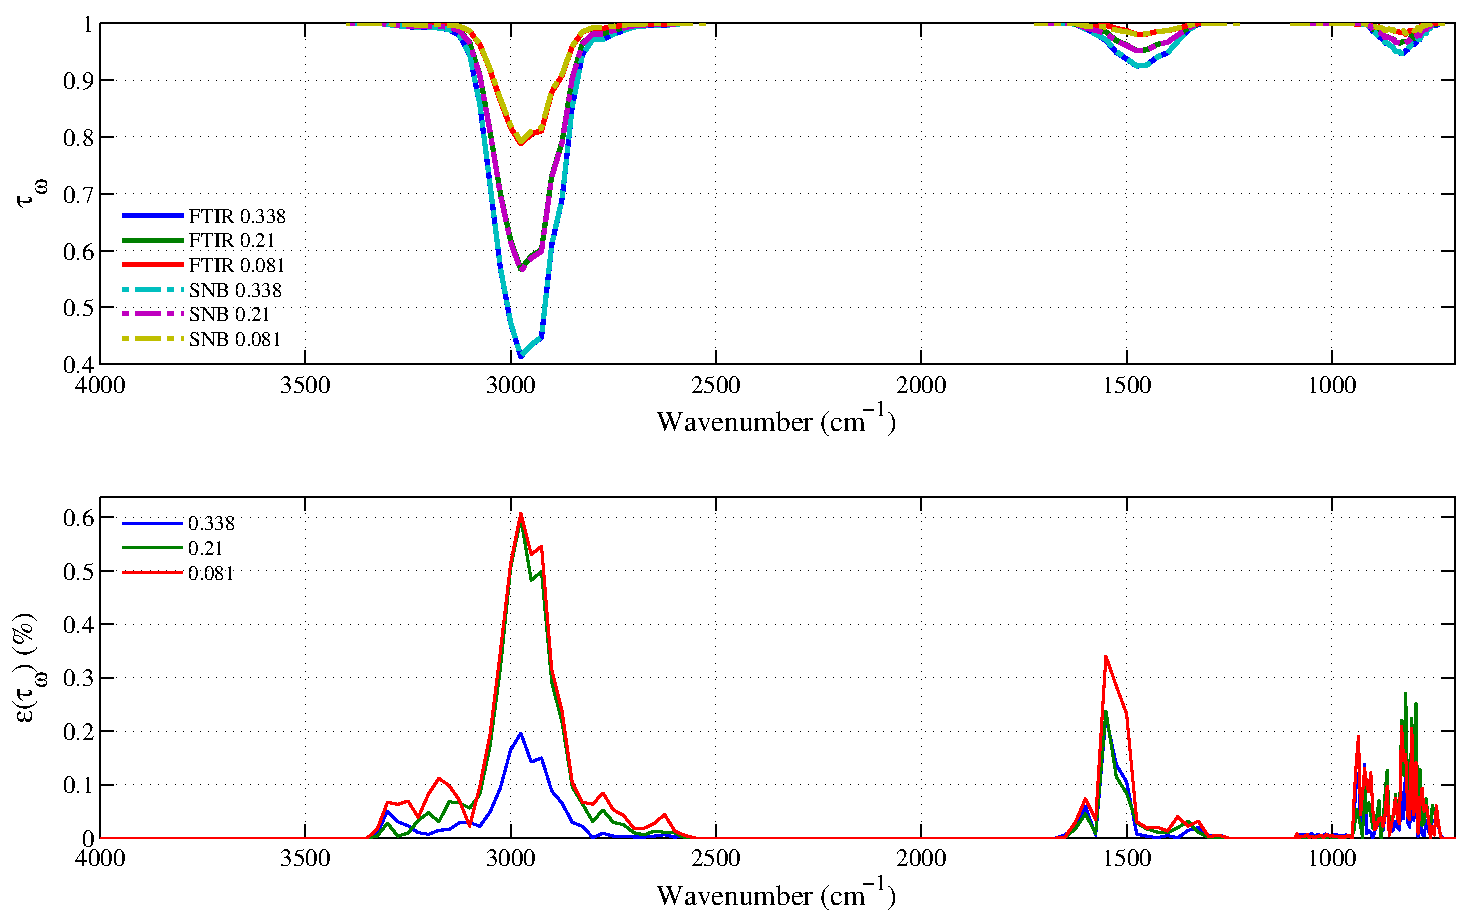
\includegraphics[width=\textwidth]{Figures/Comparison_Fit_Ethane_MALKMUS_Temp500K.pdf}
\caption{Top: comparison between the experimental (FTIR, in solid lines) and the synthetic (dashed lines) spectral transmissivity profiles, denoted $\tau_{\omega}$, of an isothermal homogeneous column of ethane. The synthetic profiles was generated using the Malkmus narrow band parameters presented in Figs.~\ref{fig:ethane_kappa_beta1} to \ref{fig:ethane_kappa_beta3}. Bottom: relative transmissivity error, denoted $\epsilon{(\tau_{\omega})}$, between the experiment and the synthetic profiles presented on the top figure. Three different pressure-paths are considered: 0.338, 0.21 and 0.081 atm.cm. The gas temperature is set at 500~K and the total pressure is 101 kPa. Note: the experimental data resolution has been changed to match that of the narrow band model. \label{fig:ethane_SNBVerify_500K}}
\end{figure}

\begin{figure}[p]
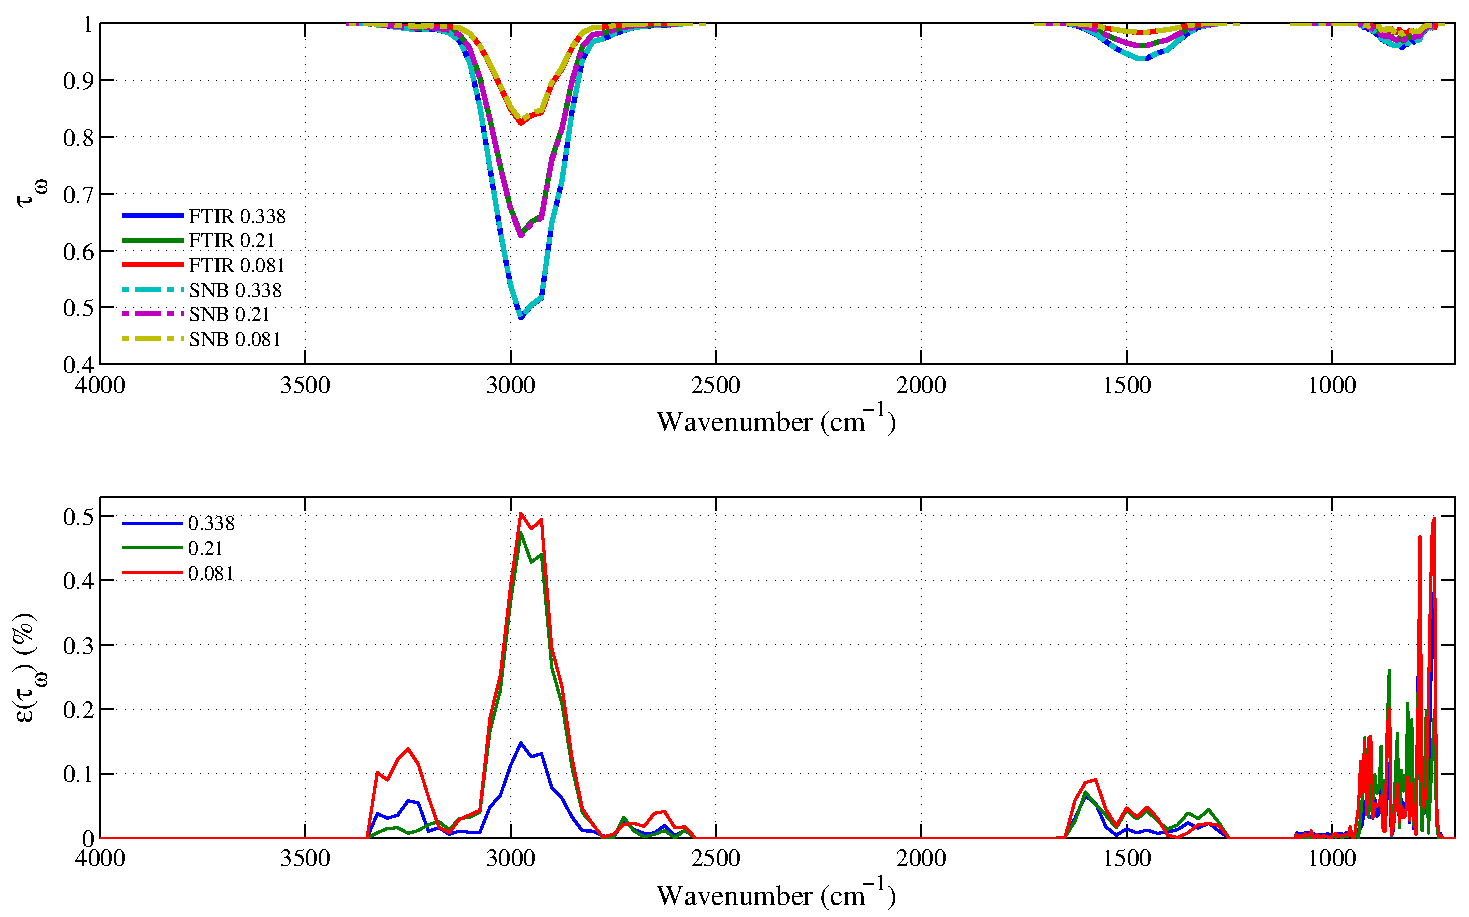
\includegraphics[width=\textwidth]{Figures/Comparison_Fit_Ethane_MALKMUS_Temp600K.pdf}
\caption{Top: comparison between the experimental (FTIR, in solid lines) and the synthetic (dashed lines) spectral transmissivity profiles, denoted $\tau_{\omega}$, of an isothermal homogeneous column of ethane. The synthetic profiles was generated using the Malkmus narrow band parameters presented in Figs.~\ref{fig:ethane_kappa_beta1} to \ref{fig:ethane_kappa_beta3}. Bottom: relative transmissivity error, denoted $\epsilon{(\tau_{\omega})}$, between the experiment and the synthetic profiles presented on the top figure. Three different pressure-paths are considered: 0.338, 0.21 and 0.081 atm.cm. The gas temperature is set at 600~K and the total pressure is 101 kPa. Note: the experimental data resolution has been changed to match that of the narrow band model. \label{fig:ethane_SNBVerify_600K}}
\end{figure}

\begin{figure}[p]
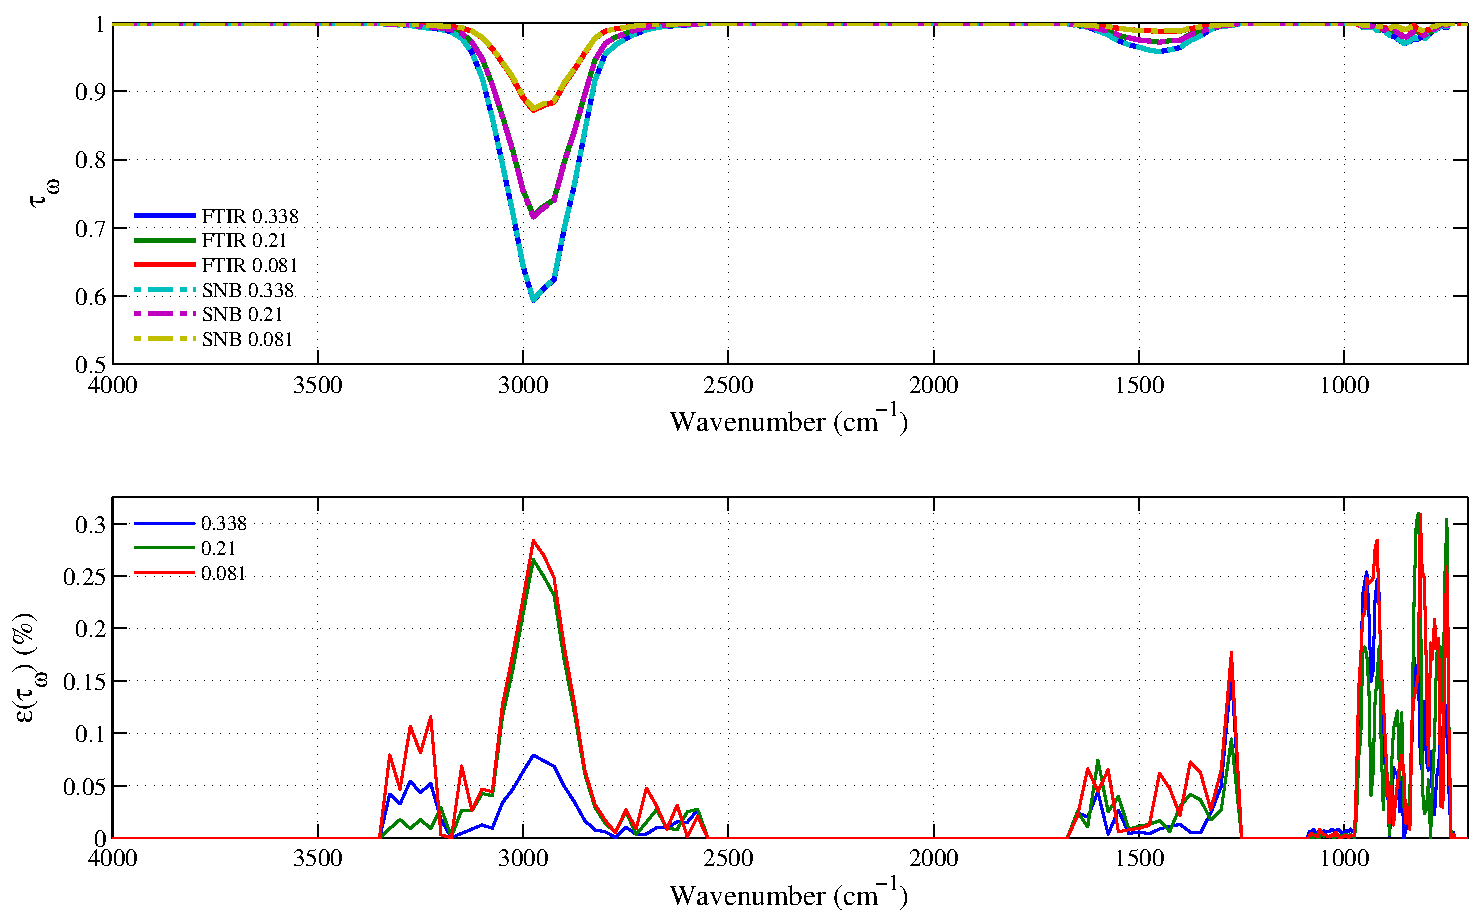
\includegraphics[width=\textwidth]{Figures/Comparison_Fit_Ethane_MALKMUS_Temp800K.pdf}
\caption{Top: comparison between the experimental (FTIR, in solid lines) and the synthetic (dashed lines) spectral transmissivity profiles, denoted $\tau_{\omega}$, of an isothermal homogeneous column of ethane. The synthetic profiles was generated using the Malkmus narrow band parameters presented in Figs.~\ref{fig:ethane_kappa_beta1} to \ref{fig:ethane_kappa_beta3}. Bottom: relative transmissivity error, denoted $\epsilon{(\tau_{\omega})}$, between the experiment and the synthetic profiles presented on the top figure. Three different pressure-paths are considered: 0.338, 0.21 and 0.081 atm.cm. The gas temperature is set at 800~K and the total pressure is 101 kPa. Note: the experimental data resolution has been changed to match that of the narrow band model. \label{fig:ethane_SNBVerify_800K}}
\end{figure}

\begin{figure}[p]
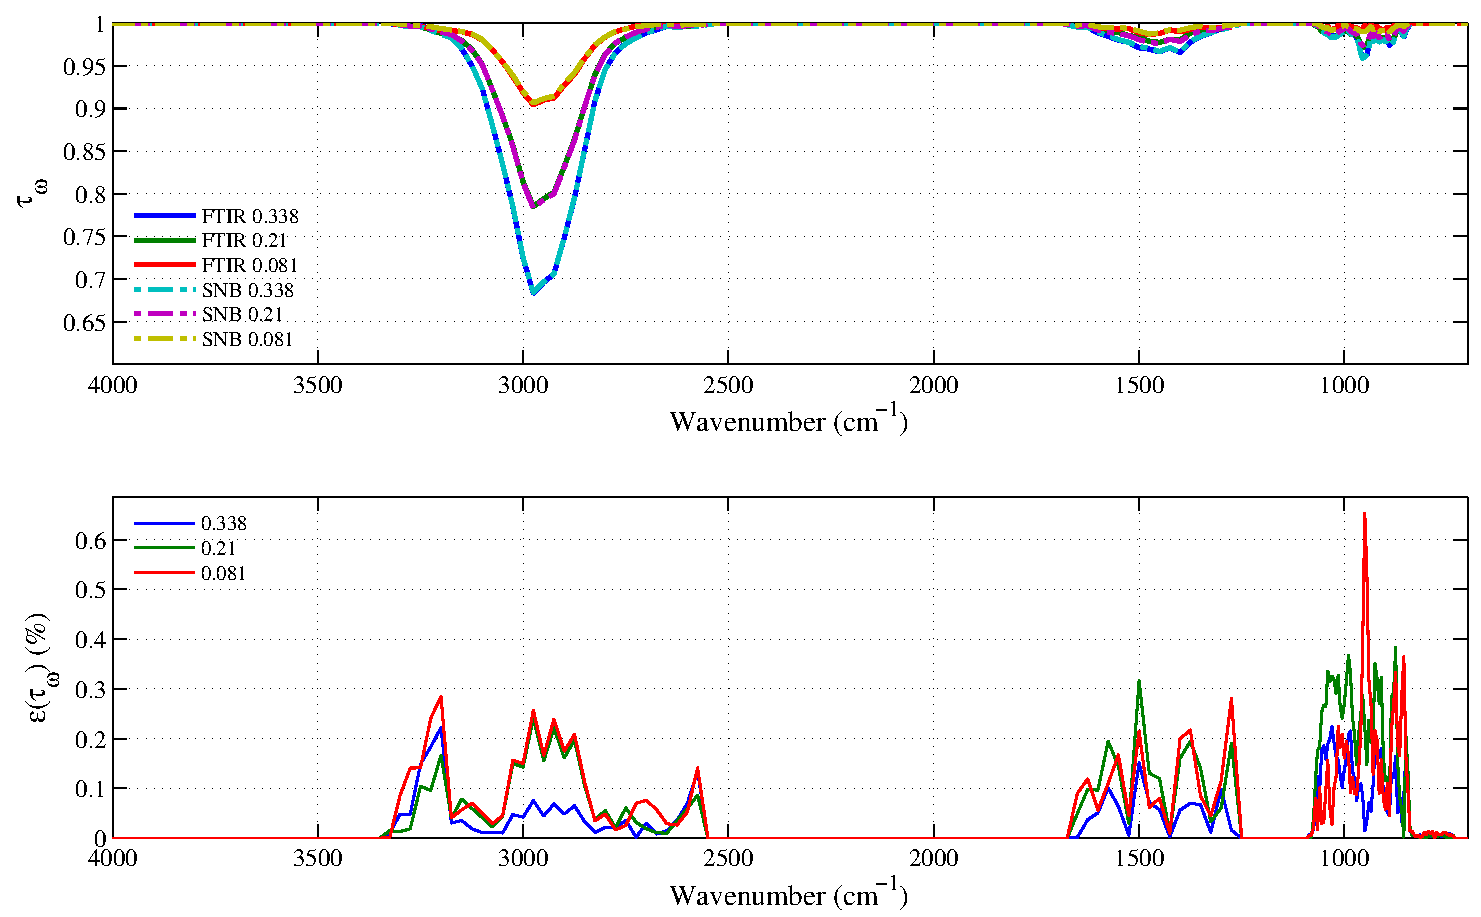
\includegraphics[width=\textwidth]{Figures/Comparison_Fit_Ethane_MALKMUS_Temp1000K.pdf}
\caption{Top: comparison between the experimental (FTIR, in solid lines) and the synthetic (dashed lines) spectral transmissivity profiles, denoted $\tau_{\omega}$, of an isothermal homogeneous column of ethane. The synthetic profiles was generated using the Malkmus narrow band parameters presented in Figs.~\ref{fig:ethane_kappa_beta1} to \ref{fig:ethane_kappa_beta3}. Bottom: relative transmissivity error, denoted $\epsilon{(\tau_{\omega})}$, between the experiment and the synthetic profiles presented on the top figure. Three different pressure-paths are considered: 0.338, 0.21 and 0.081 atm.cm. The gas temperature is set at 1000~K and the total pressure is 101 kPa. Note: the experimental data resolution has been changed to match that of the narrow band model. \label{fig:ethane_SNBVerify_1000K}}
\end{figure}


\clearpage

\section{Propylene: $\rm C_3H_6$}

\subsection{Integrated Band Intensity}

Propylene, $\rm C_3H_6$, has only one plane of symmetry and belongs to the point group $C_s$, \cite{Herzberg1949}. It has 21 vibrational modes. In RadCal, its spectrum is divided into three distinct bands, associated with different vibrational modes, see Table \ref{Table::C3H6}. The first band from 775--1150~cm$^{-1}$ is associated with the stretching motion of the carbon simple bond $\rm C-C$, the rocking motion of the $\rm CH_3$ group, and the out-of-plane bending motion of the $\rm = CH_2$ group. The second band from 1225--1975~cm$^{-1}$ is derived from the stretching motion of the carbon double bond $\rm C=C$ and the bending motion of the CH group. Finally, the third band from 2650--3275~cm$^{-1}$ is due to the stretching motion of the CH and $\rm = CH_2$ groups.

The strongest absorption bands for propylene are the 775--1150~cm$^{-1}$ (Band 1) and the 2650--3275~cm$^{-1}$ bands (Band 3). The 775--1150~cm$^{-1}$ band corresponds to radiation absorption and emission at near ambient temperature. The 2650--3275~cm$^{-1}$ band gives propylene strong absorption of radiation emitted by blackbody at high temperatures characteristic of sooting flames.

\begin{table}[ht]
   \centering
   \caption{Spectral bands of $\rm C_3H_6$ included in RadCal.}
   \vspace{0.1in}
   \label{Table::C3H6}
   \begin{tabular}{|c|c|c|c|c|}
    \hline
    Band \# & \multicolumn{2}{|l|}{Bounds (cm$\rm ^{-1}$) } & Assignment & $\alpha(T=296 \; {\rm K}) \; (\rm {atm^{-1} cm^{-2}})$\\
    \cline{1-5}
    1 & 775  & 1150 &  $\rm C-C$ Stretch, $\rm CH_3$ Rock & 296 \\
    2 & 1225 & 1975 &  $\rm C=C$ Stretch, $\rm CH$ Bend   & 271 \\
    3 & 2650 & 3275 &  $\rm CH$ \& $\rm CH_2$ Stretch      & 509 \\
    \hline
   \end{tabular}
\end{table}

\subsection{Malkmus Narrow Band Parameters}

All the propylene IR spectral absorption data were obtained from high resolution FTIR experiments with temperatures varying from 296~K to 1003~K. The spectral absorption coefficients were obtained by fitting the experimental spectral transmissivity of a homogeneous column of isothermal propylene with a total pressure of 1~atm using the Malkmus model.

The propylene narrow band parameters, $\bar{\kappa}$ and $\beta$, for temperatures ranging from 296~K to 1003~K are plotted in Figures~\ref{fig:propylene_kappa_beta1}--\ref{fig:propylene_kappa_beta3} for Bands 1 to 3.

\newpage

\begin{figure}[p]
\begin{center}
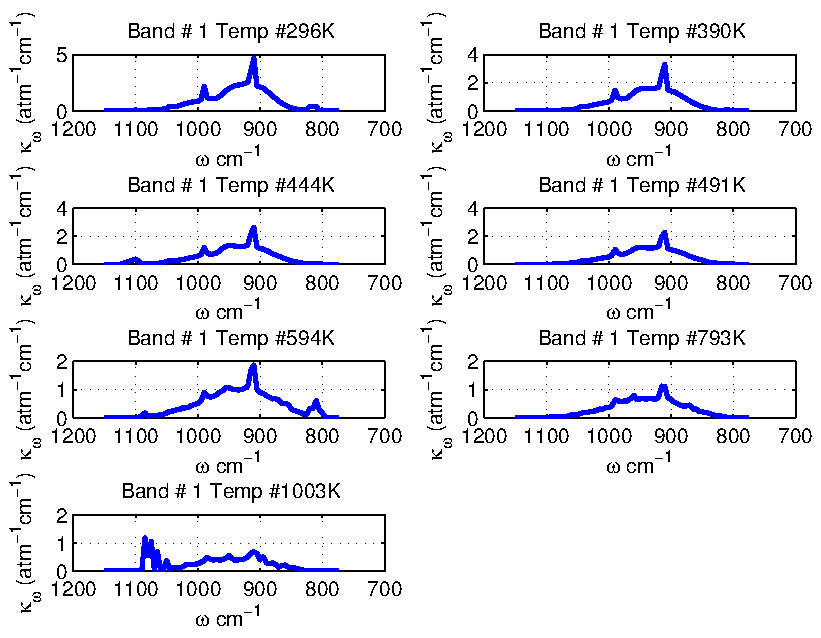
\includegraphics[width=5.0in]{Figures/Propylene_Kappa_Band1_MALKMUS.pdf}
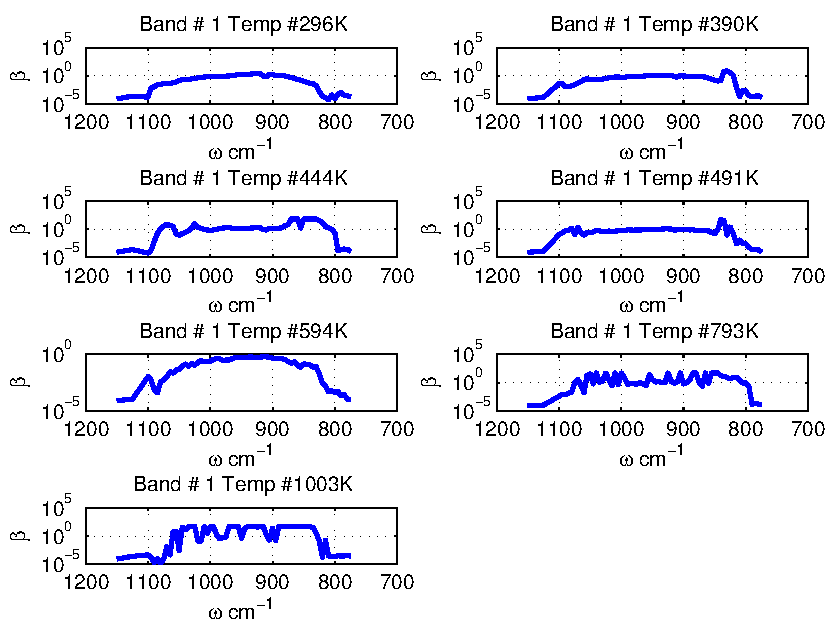
\includegraphics[width=5.0in]{Figures/Propylene_Beta_Band1_MALKMUS.pdf}
\end{center}
\caption{Propylene narrow band parameters $\bar{\kappa}$ and $\beta$ obtained for the 775--1150~cm$^{-1}$ band corresponding to the rocking motion of the $\rm CH_3$ chemical group. Temperatures plotted are: 296, 390, 444, 491, 594, 793, and 1003~K. The narrow band resolution $\Delta \om$ is 5~cm$^{-1}$.\label{fig:propylene_kappa_beta1}}
\end{figure}

\begin{figure}[p]
\begin{center}
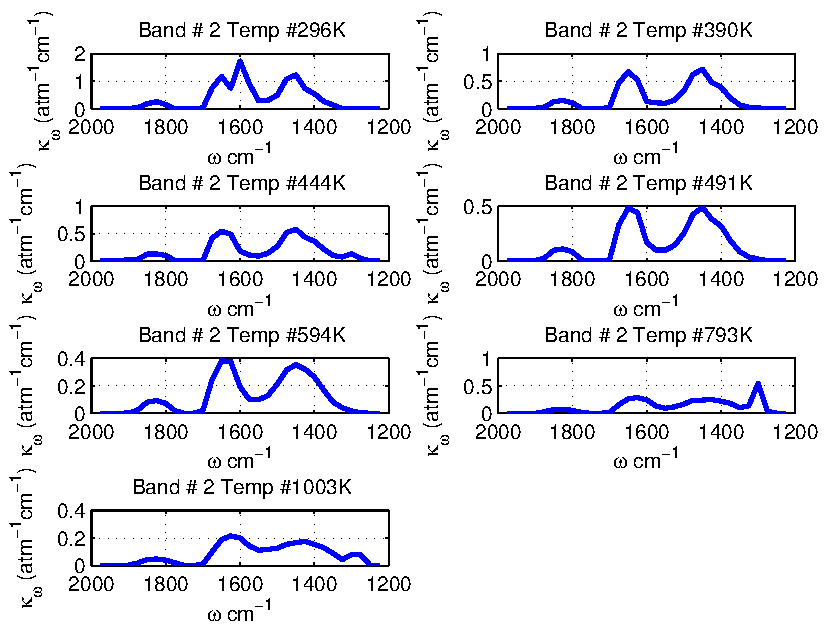
\includegraphics[width=5.0in]{Figures/Propylene_Kappa_Band2_MALKMUS.pdf}
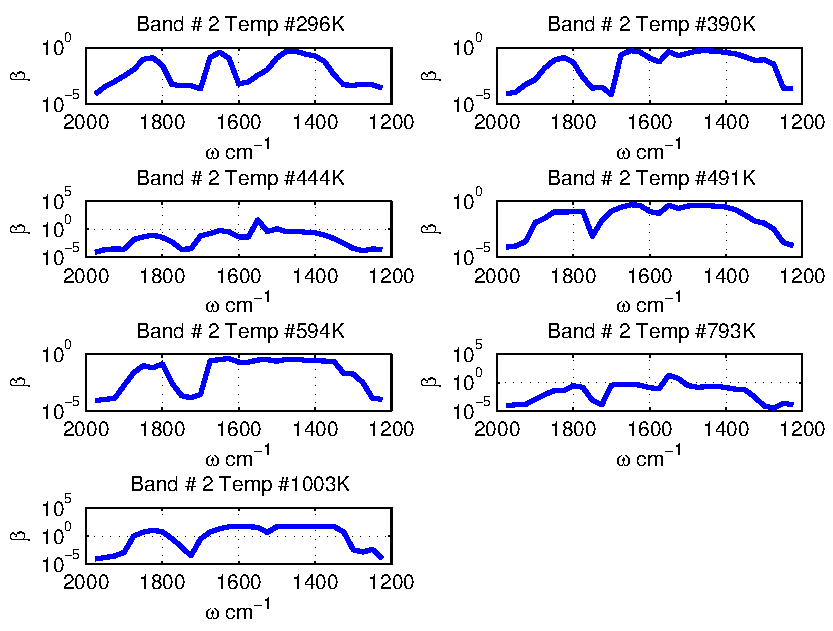
\includegraphics[width=5.0in]{Figures/Propylene_Beta_Band2_MALKMUS.pdf}
\end{center}
\caption{Propylene narrow band parameters $\bar{\kappa}$ and $\beta$ obtained for the 1225--1975~cm$^{-1}$ band corresponding to the bending motion of the $\rm CH$ chemical group. Temperatures plotted are: 296, 390, 444, 491, 594, 793, and 1003~K. The narrow band resolution $\Delta \om$ is 25~cm$^{-1}$.\label{fig:propylene_kappa_beta2}}
\end{figure}

\begin{figure}[p]
\begin{center}
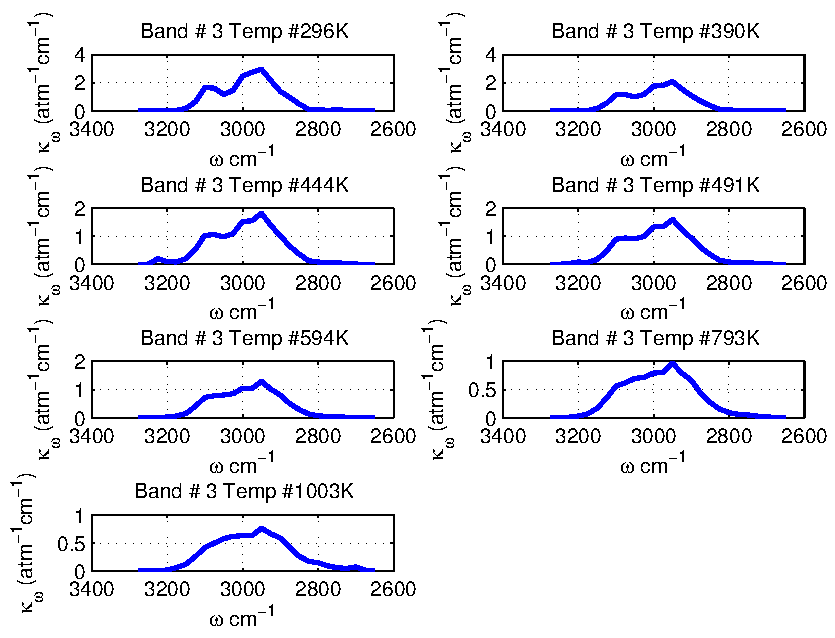
\includegraphics[width=5.0in]{Figures/Propylene_Kappa_Band3_MALKMUS.pdf}
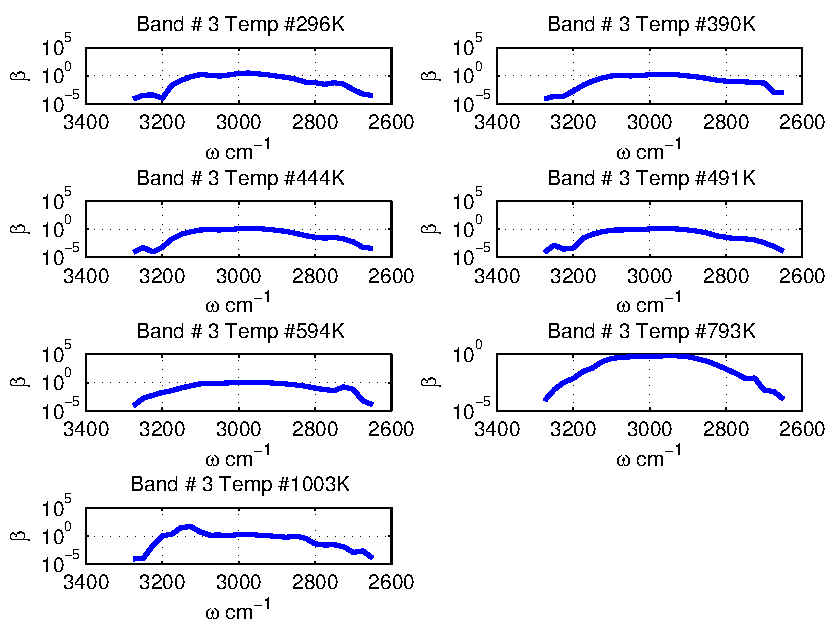
\includegraphics[width=5.0in]{Figures/Propylene_Beta_Band3_MALKMUS.pdf}
\end{center}
\caption{Propylene narrow band parameters $\bar{\kappa}$ and $\beta$ obtained for the 2650--3275~cm$^{-1}$ band corresponding to the stretching motion of the $\rm C-H$ chemical group. Temperatures plotted are: 296, 390, 444, 491, 594, 793, and 1003~K. The narrow band resolution $\Delta \om$ is 25~cm$^{-1}$.\label{fig:propylene_kappa_beta3}}
\end{figure}

\FloatBarrier

\subsection{Verification SNB Parameters}

To assess the accuracy of the narrow band parameters $\bar{\kappa}$ and $\beta$, synthetic transmissivities were constructed for the same experimental conditions as the FTIR data and compare with it. This subsection plots the comparison and the relative error in transmissivity (relative to FTIR measurements) using the propylene parameters presented in Figs.~\ref{fig:propylene_kappa_beta1} to \ref{fig:propylene_kappa_beta3}.

\begin{figure}[!h]
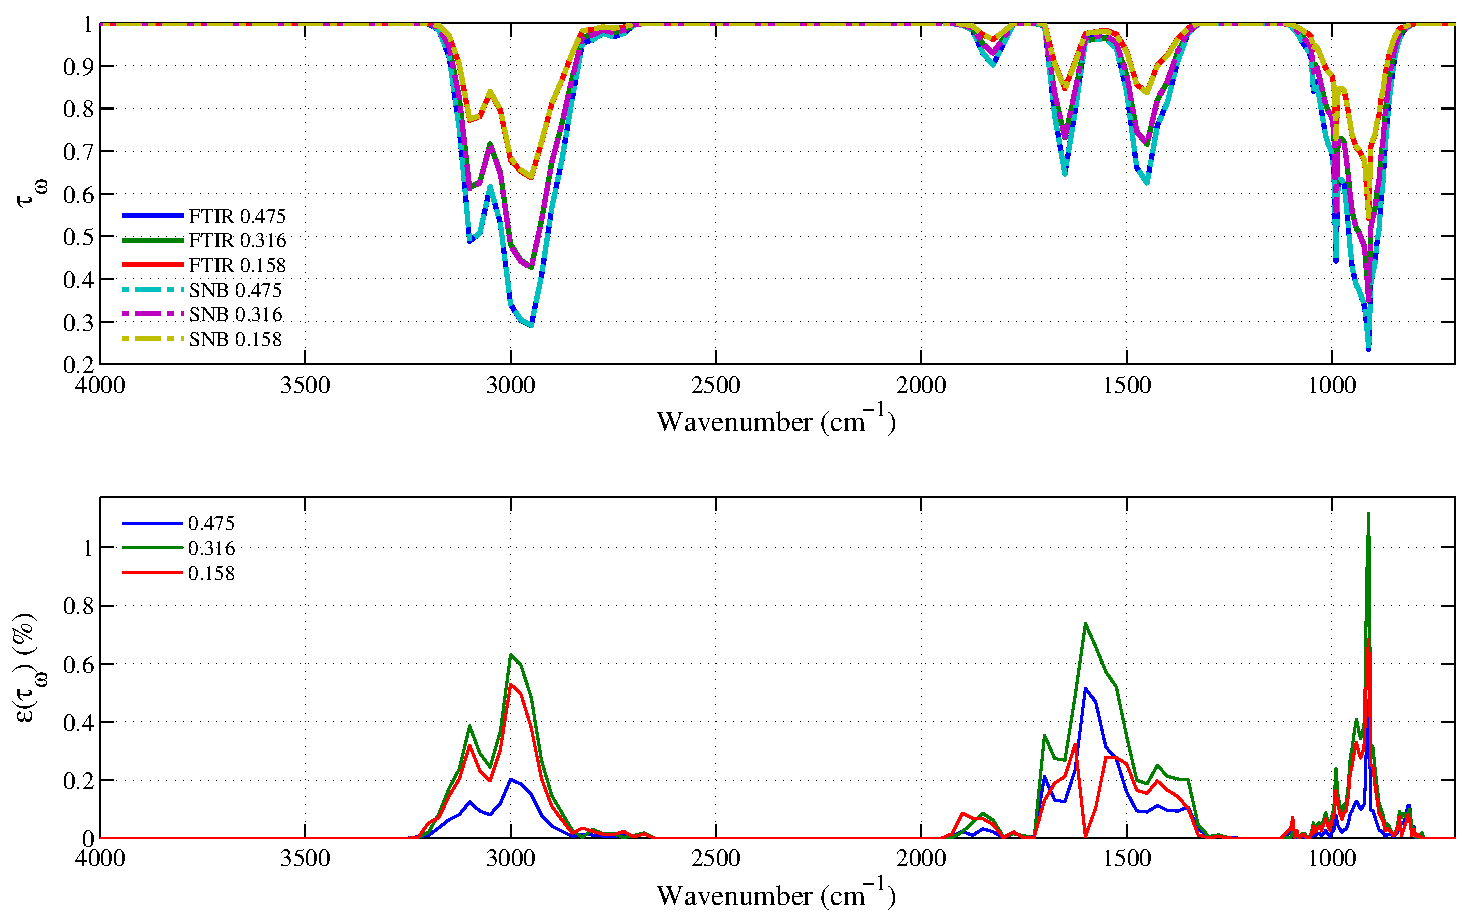
\includegraphics[width=\textwidth]{Figures/Comparison_Fit_Propylene_MALKMUS_Temp296K.pdf}
\caption{Top: comparison between the experimental (FTIR, in solid lines) and the synthetic (dashed lines) spectral transmissivity profiles, denoted $\tau_{\omega}$, of an isothermal homogeneous column of propylene. The synthetic profiles was generated using the Malkmus narrow band parameters presented in Figs.~\ref{fig:propylene_kappa_beta1} to \ref{fig:propylene_kappa_beta3}. Bottom: relative transmissivity error, denoted $\epsilon{(\tau_{\omega})}$, between the experiment and the synthetic profiles presented on the top figure. Three different pressure-paths are considered: 0.475, 0.316 and 0.158 atm.cm. The gas temperature is set at 296~K and the total pressure is 101 kPa. Note: the experimental data resolution has been changed to match that of the narrow band model. \label{fig:propylene_SNBVerify_296K}}
\end{figure}

\begin{figure}[p]
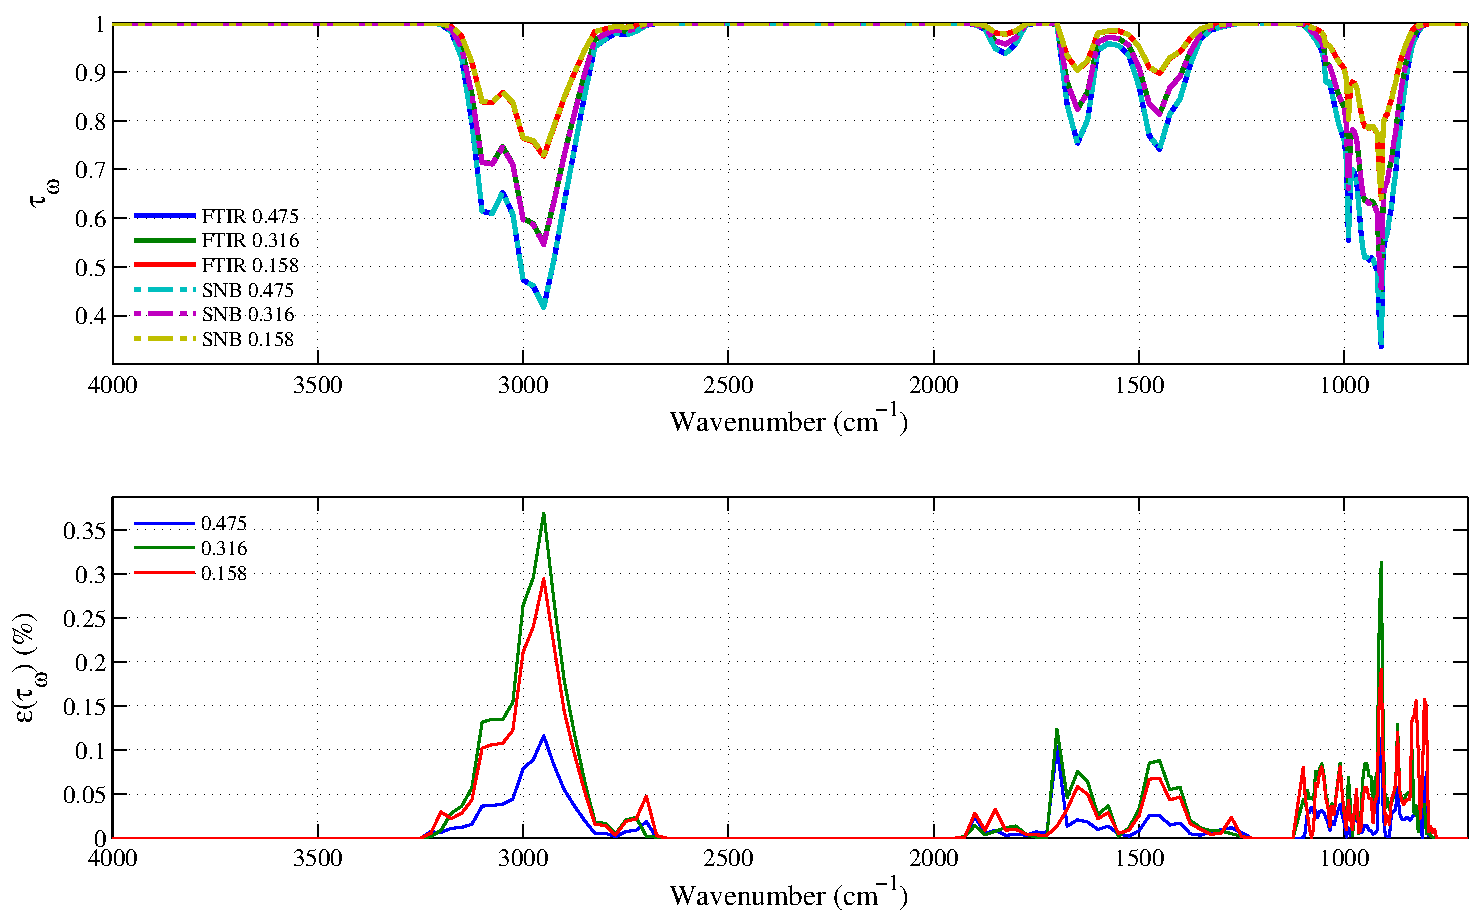
\includegraphics[width=\textwidth]{Figures/Comparison_Fit_Propylene_MALKMUS_Temp390K.pdf}
\caption{Top: comparison between the experimental (FTIR, in solid lines) and the synthetic (dashed lines) spectral transmissivity profiles, denoted $\tau_{\omega}$, of an isothermal homogeneous column of propylene. The synthetic profiles was generated using the Malkmus narrow band parameters presented in Figs.~\ref{fig:propylene_kappa_beta1} to \ref{fig:propylene_kappa_beta3}. Bottom: relative transmissivity error, denoted $\epsilon{(\tau_{\omega})}$, between the experiment and the synthetic profiles presented on the top figure. Three different pressure-paths are considered: 0.475, 0.316 and 0.158 atm.cm. The gas temperature is set at 390~K and the total pressure is 101 kPa. Note: the experimental data resolution has been changed to match that of the narrow band model. \label{fig:propylene_SNBVerify_390K}}
\end{figure}

\begin{figure}[p]
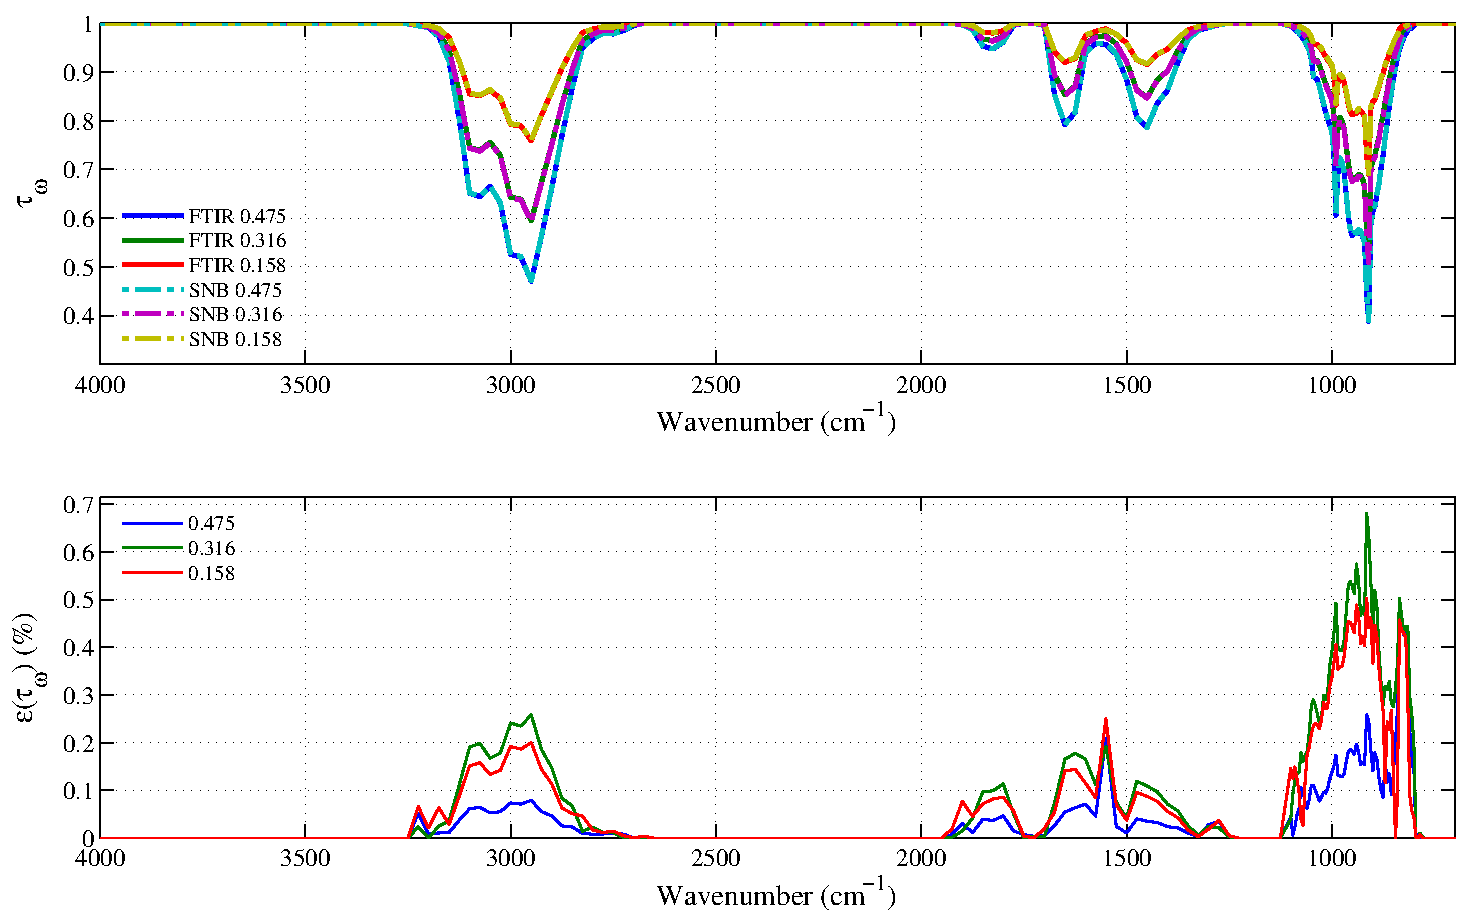
\includegraphics[width=\textwidth]{Figures/Comparison_Fit_Propylene_MALKMUS_Temp444K.pdf}
\caption{Top: comparison between the experimental (FTIR, in solid lines) and the synthetic (dashed lines) spectral transmissivity profiles, denoted $\tau_{\omega}$, of an isothermal homogeneous column of propylene. The synthetic profiles was generated using the Malkmus narrow band parameters presented in Figs.~\ref{fig:propylene_kappa_beta1} to \ref{fig:propylene_kappa_beta3}. Bottom: relative transmissivity error, denoted $\epsilon{(\tau_{\omega})}$, between the experiment and the synthetic profiles presented on the top figure. Three different pressure-paths are considered: 0.475, 0.316 and 0.158 atm.cm. The gas temperature is set at 444~K and the total pressure is 101 kPa. Note: the experimental data resolution has been changed to match that of the narrow band model. \label{fig:propylene_SNBVerify_444K}}
\end{figure}

\begin{figure}[p]
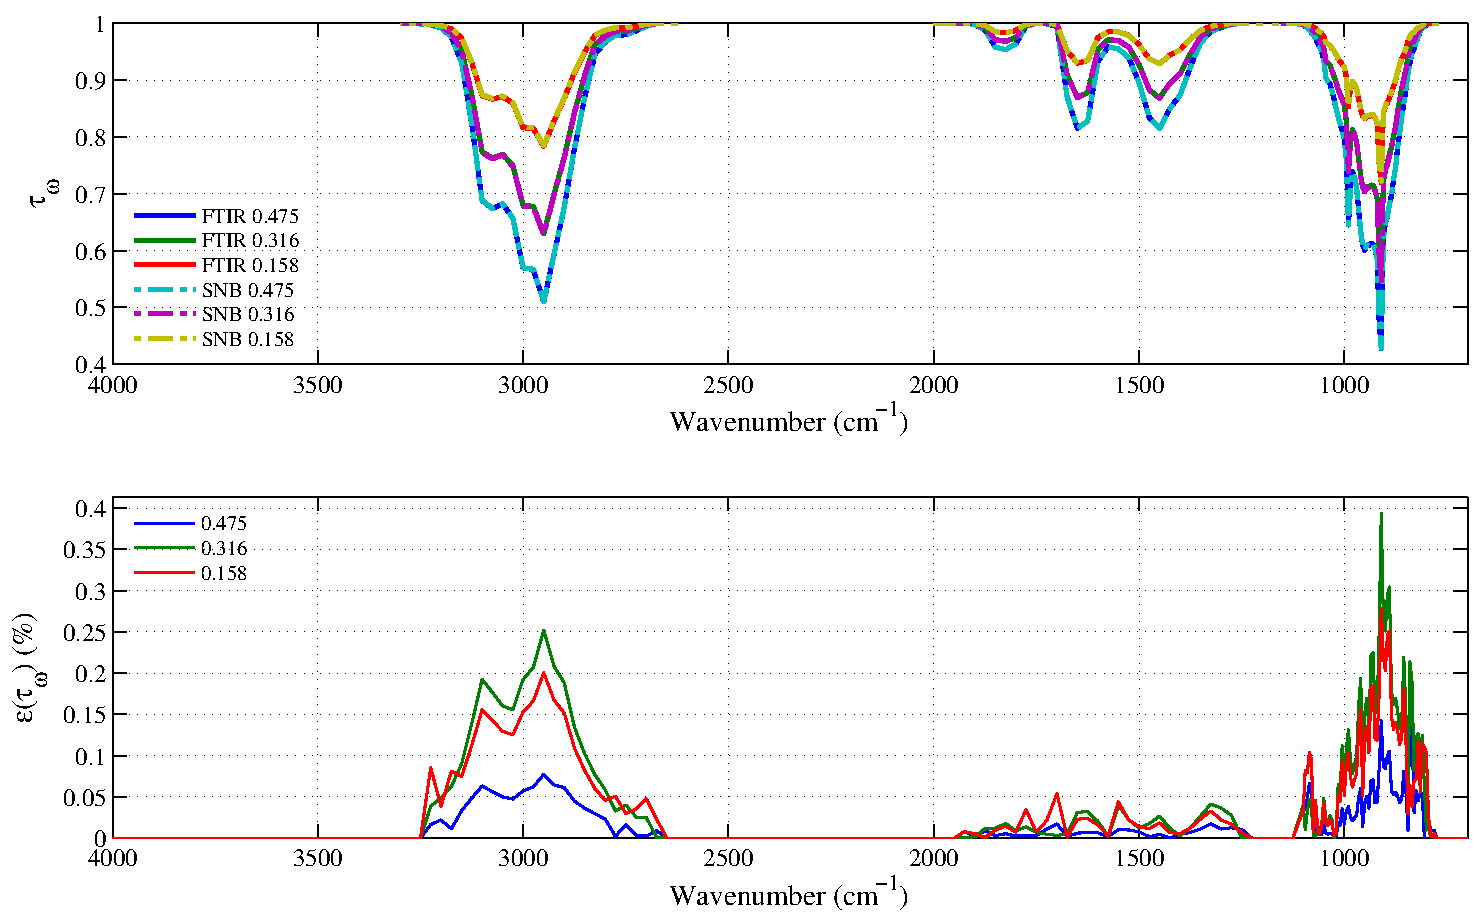
\includegraphics[width=\textwidth]{Figures/Comparison_Fit_Propylene_MALKMUS_Temp491K.pdf}
\caption{Top: comparison between the experimental (FTIR, in solid lines) and the synthetic (dashed lines) spectral transmissivity profiles, denoted $\tau_{\omega}$, of an isothermal homogeneous column of propylene. The synthetic profiles was generated using the Malkmus narrow band parameters presented in Figs.~\ref{fig:propylene_kappa_beta1} to \ref{fig:propylene_kappa_beta3}. Bottom: relative transmissivity error, denoted $\epsilon{(\tau_{\omega})}$, between the experiment and the synthetic profiles presented on the top figure. Three different pressure-paths are considered: 0.475, 0.316 and 0.158 atm.cm. The gas temperature is set at 491~K and the total pressure is 101 kPa. Note: the experimental data resolution has been changed to match that of the narrow band model. \label{fig:propylene_SNBVerify_491K}}
\end{figure}

\begin{figure}[p]
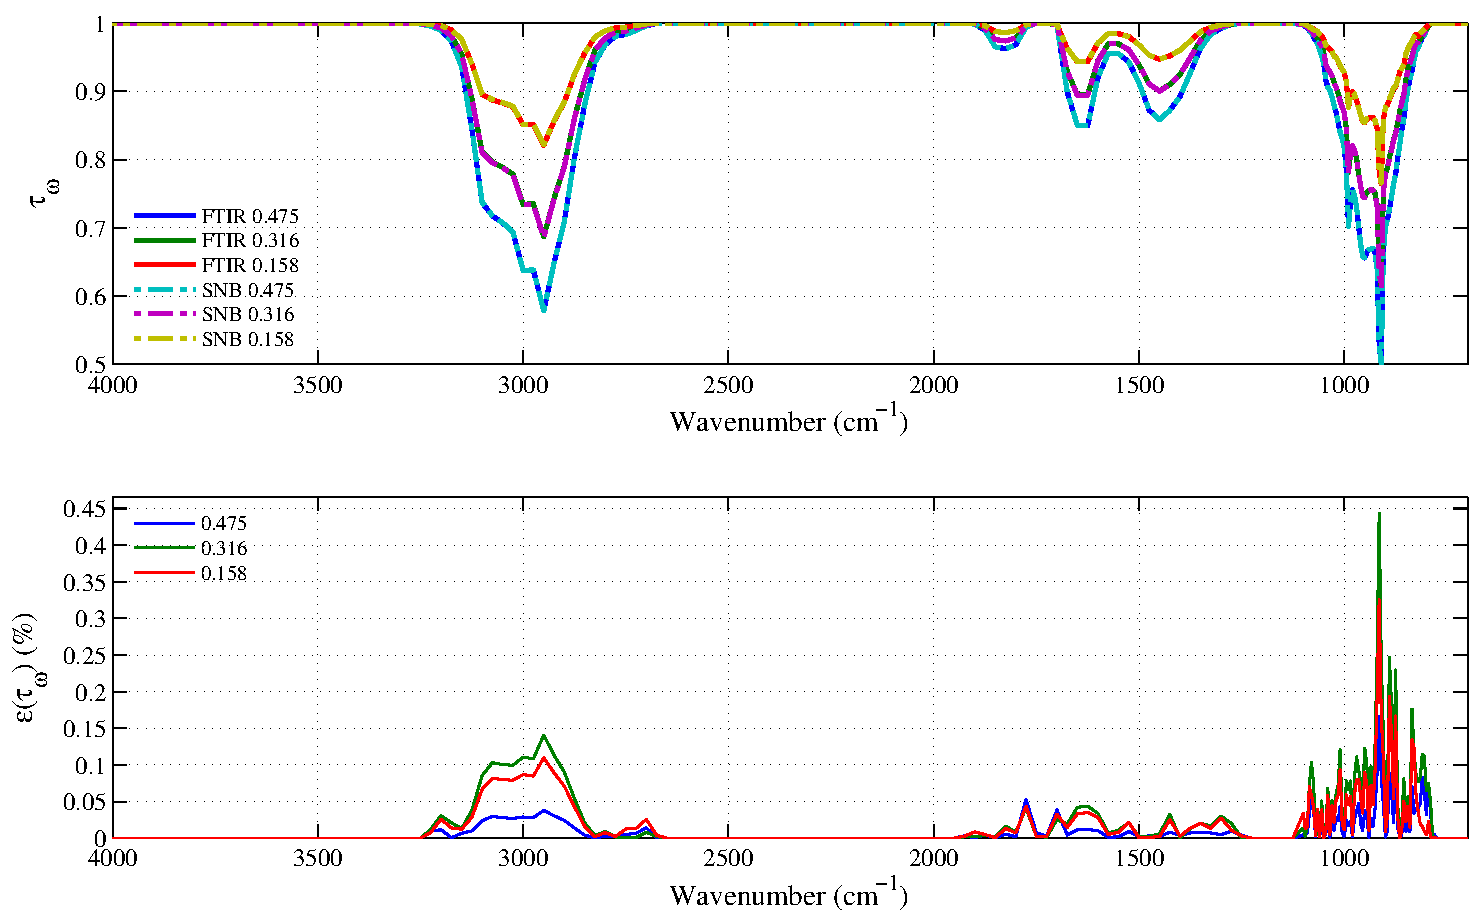
\includegraphics[width=\textwidth]{Figures/Comparison_Fit_Propylene_MALKMUS_Temp594K.pdf}
\caption{Top: comparison between the experimental (FTIR, in solid lines) and the synthetic (dashed lines) spectral transmissivity profiles, denoted $\tau_{\omega}$, of an isothermal homogeneous column of propylene. The synthetic profiles was generated using the Malkmus narrow band parameters presented in Figs.~\ref{fig:propylene_kappa_beta1} to \ref{fig:propylene_kappa_beta3}. Bottom: relative transmissivity error, denoted $\epsilon{(\tau_{\omega})}$, between the experiment and the synthetic profiles presented on the top figure. Three different pressure-paths are considered: 0.475, 0.316 and 0.158 atm.cm. The gas temperature is set at 594~K and the total pressure is 101 kPa. Note: the experimental data resolution has been changed to match that of the narrow band model. \label{fig:propylene_SNBVerify_594K}}
\end{figure}

\begin{figure}[p]
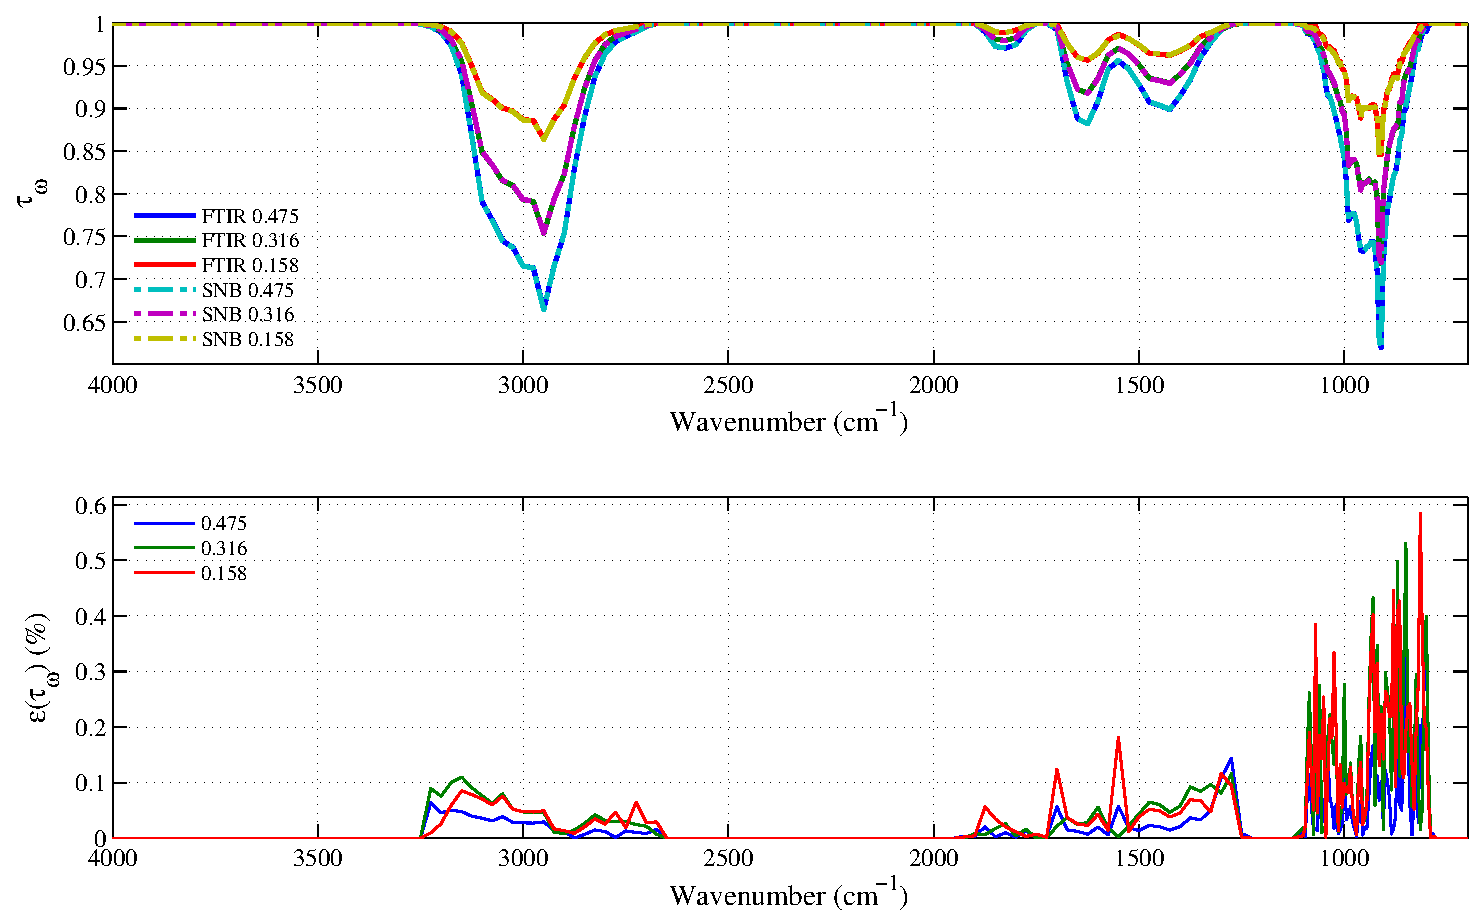
\includegraphics[width=\textwidth]{Figures/Comparison_Fit_Propylene_MALKMUS_Temp793K.pdf}
\caption{Top: comparison between the experimental (FTIR, in solid lines) and the synthetic (dashed lines) spectral transmissivity profiles, denoted $\tau_{\omega}$, of an isothermal homogeneous column of propylene. The synthetic profiles was generated using the Malkmus narrow band parameters presented in Figs.~\ref{fig:propylene_kappa_beta1} to \ref{fig:propylene_kappa_beta3}. Bottom: relative transmissivity error, denoted $\epsilon{(\tau_{\omega})}$, between the experiment and the synthetic profiles presented on the top figure. Three different pressure-paths are considered: 0.475, 0.316 and 0.158 atm.cm. The gas temperature is set at 793~K and the total pressure is 101 kPa. Note: the experimental data resolution has been changed to match that of the narrow band model. \label{fig:propylene_SNBVerify_793K}}
\end{figure}

\begin{figure}[p]
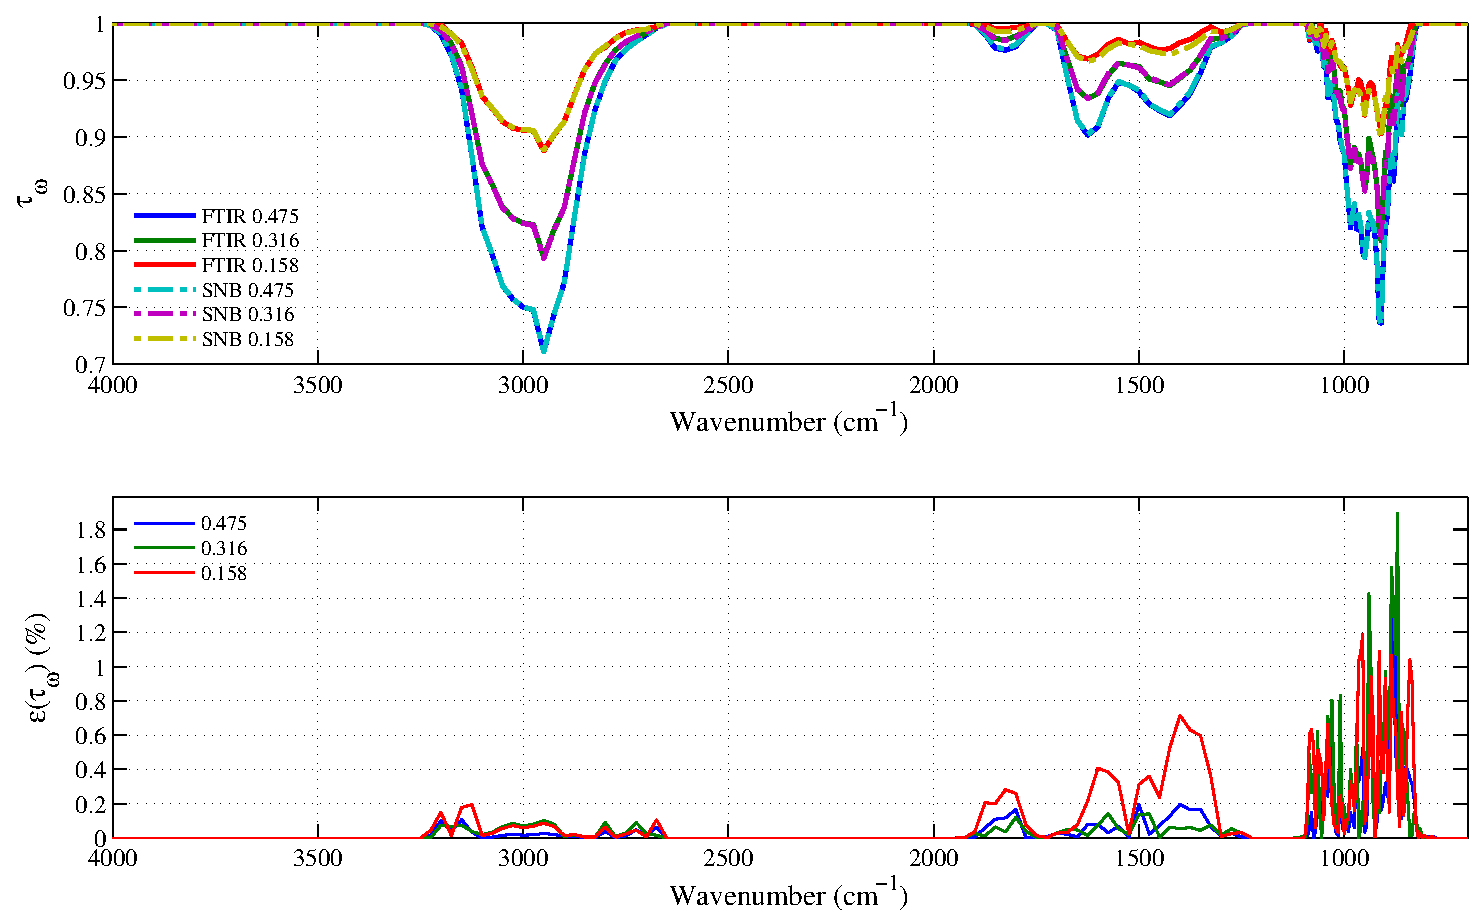
\includegraphics[width=\textwidth]{Figures/Comparison_Fit_Propylene_MALKMUS_Temp1003K.pdf}
\caption{Top: comparison between the experimental (FTIR, in solid lines) and the synthetic (dashed lines) spectral transmissivity profiles, denoted $\tau_{\omega}$, of an isothermal homogeneous column of propylene. The synthetic profiles was generated using the Malkmus narrow band parameters presented in Figs.~\ref{fig:propylene_kappa_beta1} to \ref{fig:propylene_kappa_beta3}. Bottom: relative transmissivity error, denoted $\epsilon{(\tau_{\omega})}$, between the experiment and the synthetic profiles presented on the top figure. Three different pressure-paths are considered: 0.475, 0.316 and 0.158 atm.cm. The gas temperature is set at 1003~K and the total pressure is 101 kPa. Note: the experimental data resolution has been changed to match that of the narrow band model. \label{fig:propylene_SNBVerify_1003K}}
\end{figure}


\clearpage

\section{Propane: $\rm C_3H_8$}

\subsection{Integrated Band Intensity}

Propane, $\rm C_3H_8$, has two planes of symmetry and two axes of rotation and belongs to the point group $C_{2v}$ \cite{Herzberg1949}. It has 27 vibrational modes. In RadCal, its spectrum is divided into two distinct bands, associated with different vibrational modes, see Table \ref{Table::C3H8}. The propane IR spectrum is the result of the vibration-rotation modes of the $\rm C-C$, $\rm CH_2$, $\rm CH_3$ groups.
The first band from 1175--1675~cm$\rm ^{-1}$ is associated with the bending motion of the $\rm CH_3$ chemical group. The second band from 2550--3375~cm$\rm ^{-1}$ is associated with the stretching motion of the chemical groups $\rm CH_3$ and $\rm CH_2$. It is the strongest band; its integrated band intensity is about 10 times that of the 1175--1675~cm$\rm ^{-1}$ band.

\begin{table}[ht]
   \centering
   \caption{Spectral bands of $\rm C_3H_8$ included in RadCal.}
   \vspace{0.1in}
   \label{Table::C3H8}
   \begin{tabular}{|c|c|c|c|c|}
    \hline
    Band \# & \multicolumn{2}{|l|}{Bounds (cm$\rm ^{-1}$) } & Assignment & $\alpha(T=295 \; {\rm K}) \; (\rm {atm^{-1} cm^{-2}})$ \\
    \cline{1-5}
    1 & 1175 & 1675 &  $\rm CH_3$ Bending        & 122 \\
    2 & 2550 & 3375 &  $\rm CH_3, CH_2$ Stretch  & 1191 \\
    \hline
   \end{tabular}
\end{table}

\subsection{Malkmus Narrow Band Parameters}

All the propane IR spectral absorption data were obtained from high resolution FTIR experiments with temperatures varying from 295~K to 1009~K. The spectral absorption coefficients were obtained by fitting the experimental spectral transmissivity of a homogeneous column of isothermal propane with a total pressure of 1~atm using the Malkmus model.

The propane narrow band parameters, $\bar{\kappa}$ and $\beta$, for temperatures ranging from 295~K to 1009~K are plotted in Figures~\ref{fig:propane_kappa_beta1}--\ref{fig:propane_kappa_beta2} for Bands 1 to 2.

\newpage

\begin{figure}[p]
\begin{center}
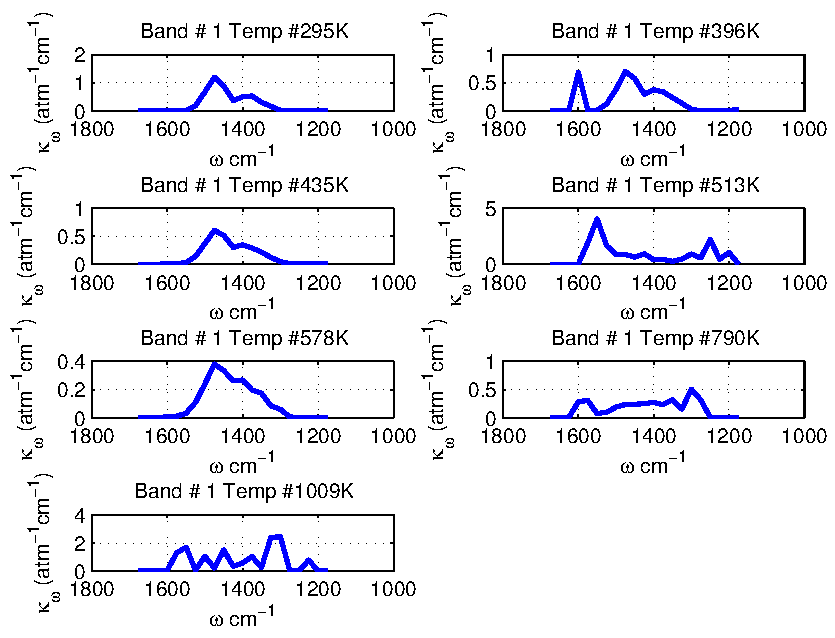
\includegraphics[width=5.0in]{Figures/Propane_Kappa_Band1_MALKMUS.pdf}
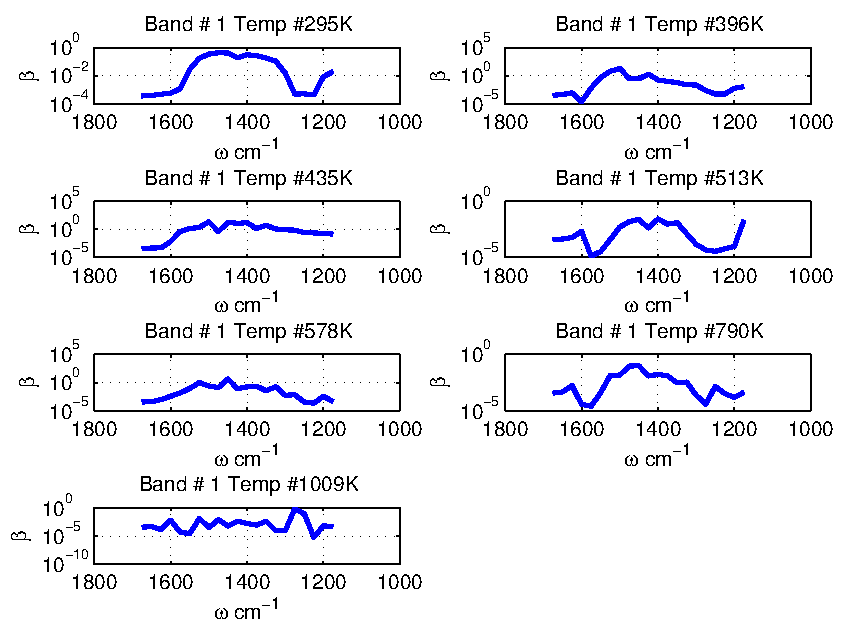
\includegraphics[width=5.0in]{Figures/Propane_Beta_Band1_MALKMUS.pdf}
\end{center}
\caption{Propane narrow band parameters $\bar{\kappa}$ and $\beta$ obtained for the 1175--1675~cm$^{-1}$ band corresponding to the bending motion of the $\rm CH_3$ chemical group. Temperatures plotted are: 295, 396, 435, 513, 578, 790, and 1009~K. The narrow band resolution $\Delta \om$ is 5~cm$^{-1}$.\label{fig:propane_kappa_beta1}}
\end{figure}

\begin{figure}[p]
\begin{center}
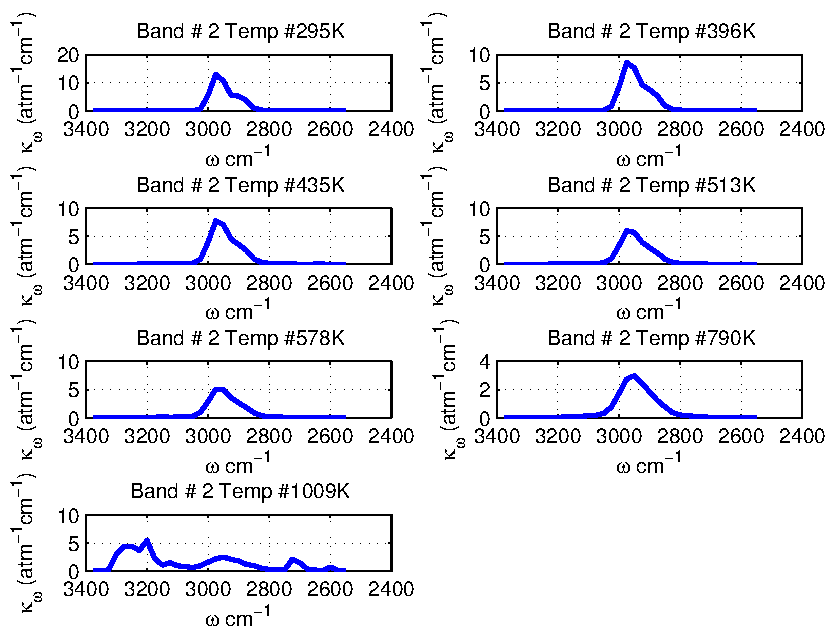
\includegraphics[width=5.0in]{Figures/Propane_Kappa_Band2_MALKMUS.pdf}
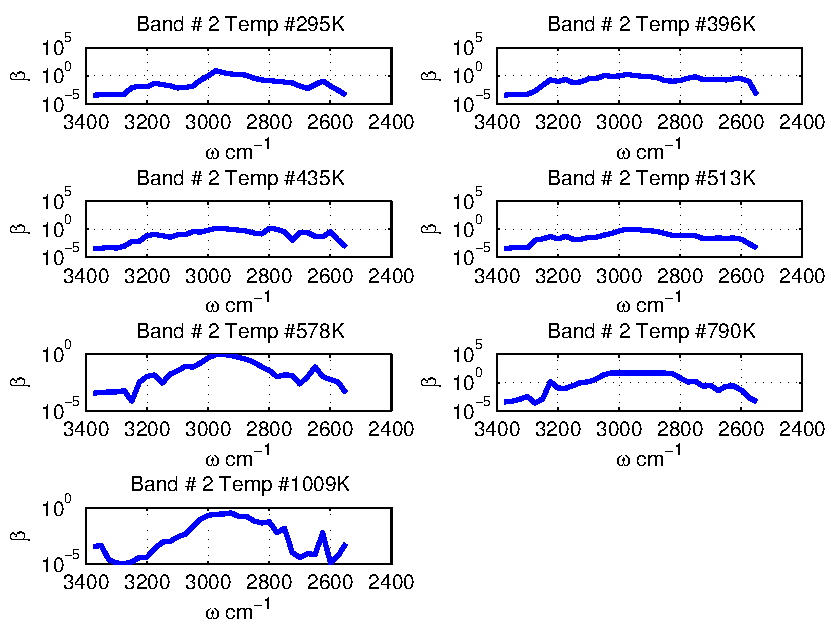
\includegraphics[width=5.0in]{Figures/Propane_Beta_Band2_MALKMUS.pdf}
\end{center}
\caption{Propane narrow band parameters $\bar{\kappa}$ and $\beta$ obtained for the 2550--3375~cm$^{-1}$ band corresponding to the bending motion of the $\rm CH$ chemical group. Temperatures plotted are: 295, 396, 435, 513, 578, 790, and 1009~K. The narrow band resolution $\Delta \om$ is 25~cm$^{-1}$.\label{fig:propane_kappa_beta2}}
\end{figure}

\FloatBarrier

\subsection{Verification SNB Parameters}

To assess the accuracy of the narrow band parameters $\bar{\kappa}$ and $\beta$, synthetic transmissivities were constructed for the same experimental conditions as the FTIR data and compare with it. This subsection plots the comparison and the relative error in transmissivity (relative to FTIR measurements) using the propane parameters presented in Figs.~\ref{fig:propane_kappa_beta1} to \ref{fig:propane_kappa_beta2}.

\begin{figure}[!h]
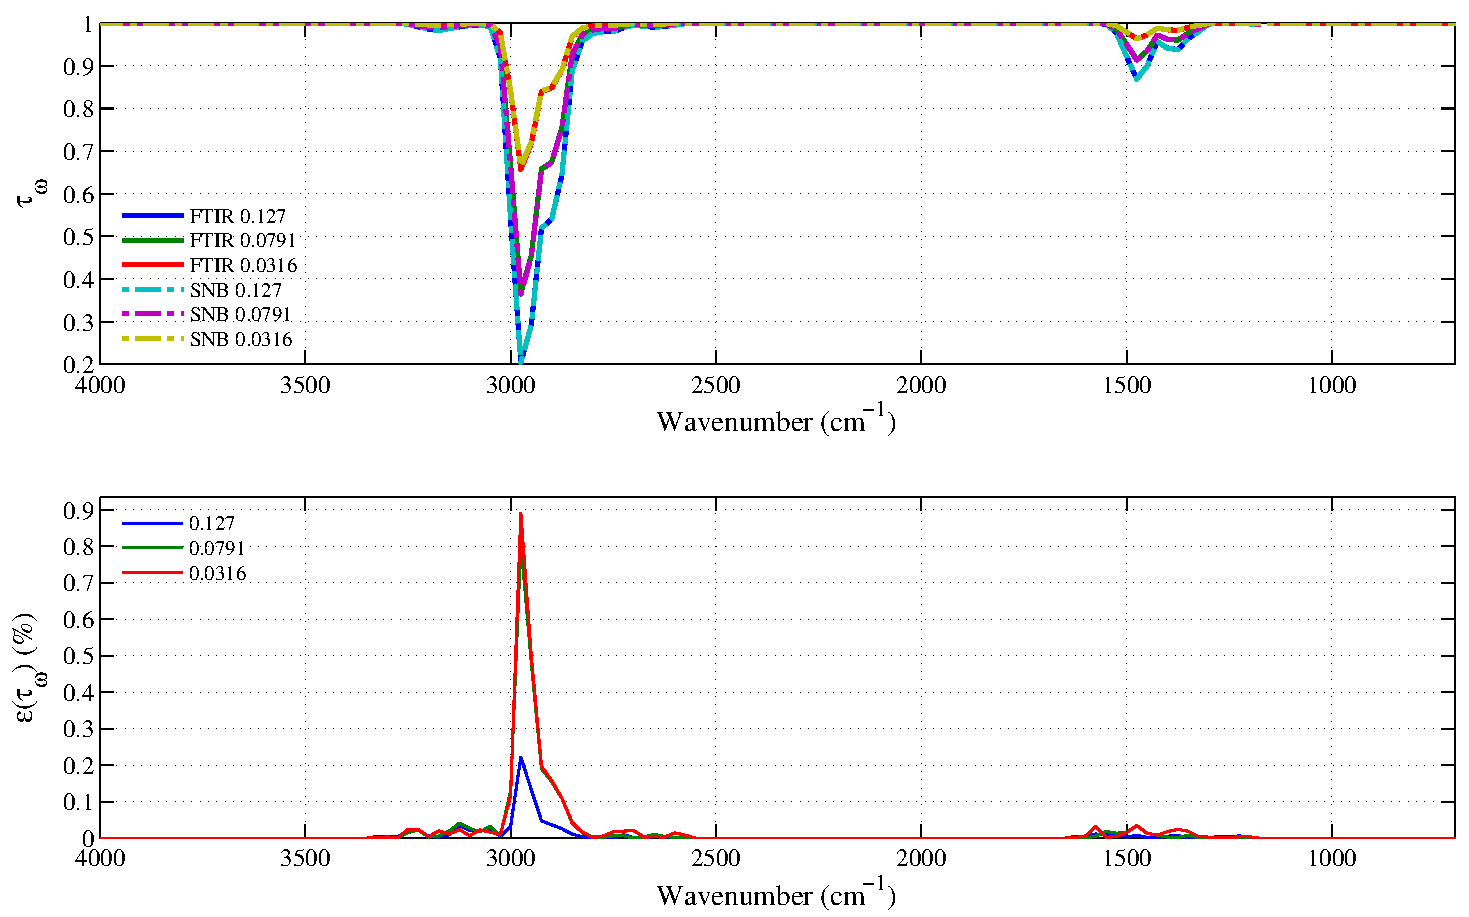
\includegraphics[width=\textwidth]{Figures/Comparison_Fit_Propane_MALKMUS_Temp295K.pdf}
\caption{Top: comparison between the experimental (FTIR, in solid lines) and the synthetic (dashed lines) spectral transmissivity profiles, denoted $\tau_{\omega}$, of an isothermal homogeneous column of propane. The synthetic profiles was generated using the Malkmus narrow band parameters presented in Figs.~\ref{fig:propane_kappa_beta1} to \ref{fig:propane_kappa_beta2}. Bottom: relative transmissivity error, denoted $\epsilon{(\tau_{\omega})}$, between the experiment and the synthetic profiles presented on the top figure. Three different pressure-paths are considered: 0.127, 0.0791 and 0.0316 atm.cm. The gas temperature is set at 295~K and the total pressure is 101 kPa. Note: the experimental data resolution has been changed to match that of the narrow band model. \label{fig:propane_SNBVerify_295K}}
\end{figure}

\begin{figure}[p]
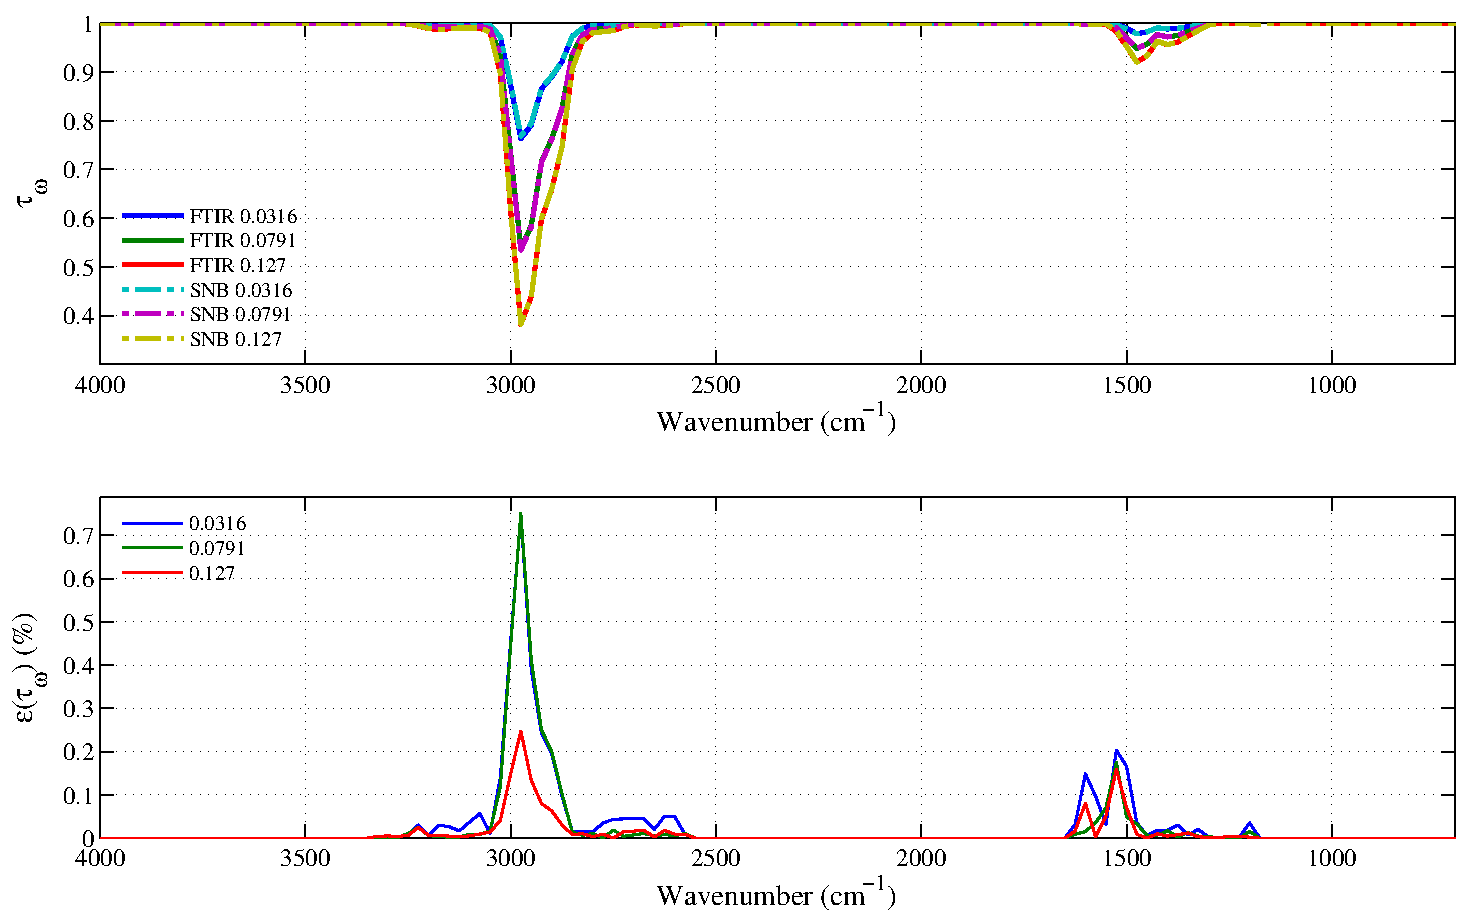
\includegraphics[width=\textwidth]{Figures/Comparison_Fit_Propane_MALKMUS_Temp396K.pdf}
\caption{Top: comparison between the experimental (FTIR, in solid lines) and the synthetic (dashed lines) spectral transmissivity profiles, denoted $\tau_{\omega}$, of an isothermal homogeneous column of propane. The synthetic profiles was generated using the Malkmus narrow band parameters presented in Figs.~\ref{fig:propane_kappa_beta1} to \ref{fig:propane_kappa_beta2}. Bottom: relative transmissivity error, denoted $\epsilon{(\tau_{\omega})}$, between the experiment and the synthetic profiles presented on the top figure. Three different pressure-paths are considered: 0.127, 0.0791 and 0.0316 atm.cm. The gas temperature is set at 396~K and the total pressure is 101 kPa. Note: the experimental data resolution has been changed to match that of the narrow band model. \label{fig:propane_SNBVerify_396K}}
\end{figure}

\begin{figure}[p]
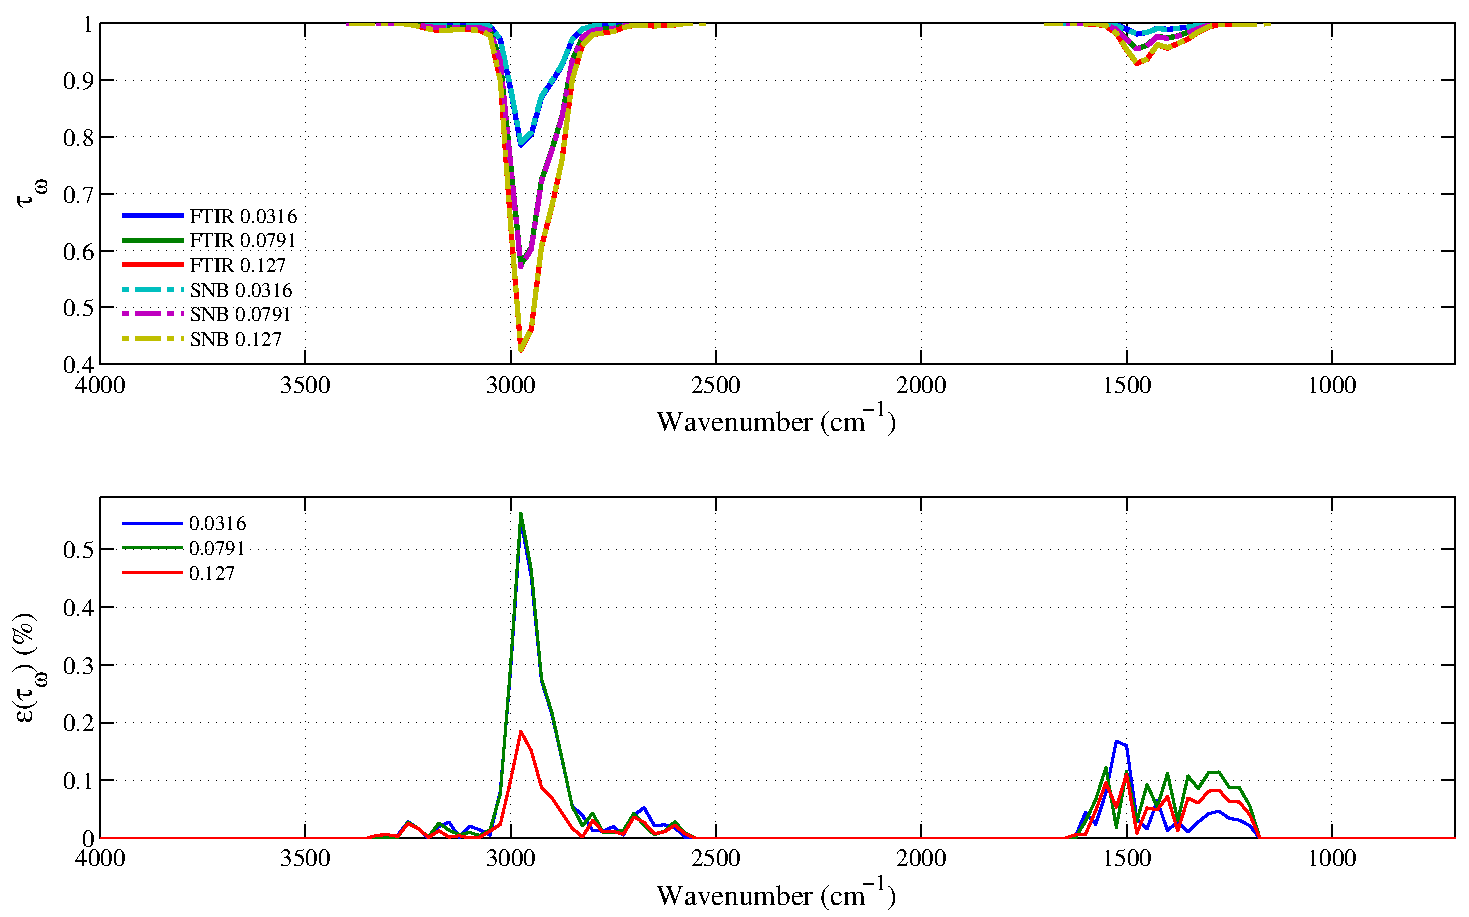
\includegraphics[width=\textwidth]{Figures/Comparison_Fit_Propane_MALKMUS_Temp435K.pdf}
\caption{Top: comparison between the experimental (FTIR, in solid lines) and the synthetic (dashed lines) spectral transmissivity profiles, denoted $\tau_{\omega}$, of an isothermal homogeneous column of propane. The synthetic profiles was generated using the Malkmus narrow band parameters presented in Figs.~\ref{fig:propane_kappa_beta1} to \ref{fig:propane_kappa_beta2}. Bottom: relative transmissivity error, denoted $\epsilon{(\tau_{\omega})}$, between the experiment and the synthetic profiles presented on the top figure. Three different pressure-paths are considered: 0.127, 0.0791 and 0.0316 atm.cm. The gas temperature is set at 435~K and the total pressure is 101 kPa. Note: the experimental data resolution has been changed to match that of the narrow band model. \label{fig:propane_SNBVerify_435K}}
\end{figure}

\begin{figure}[p]
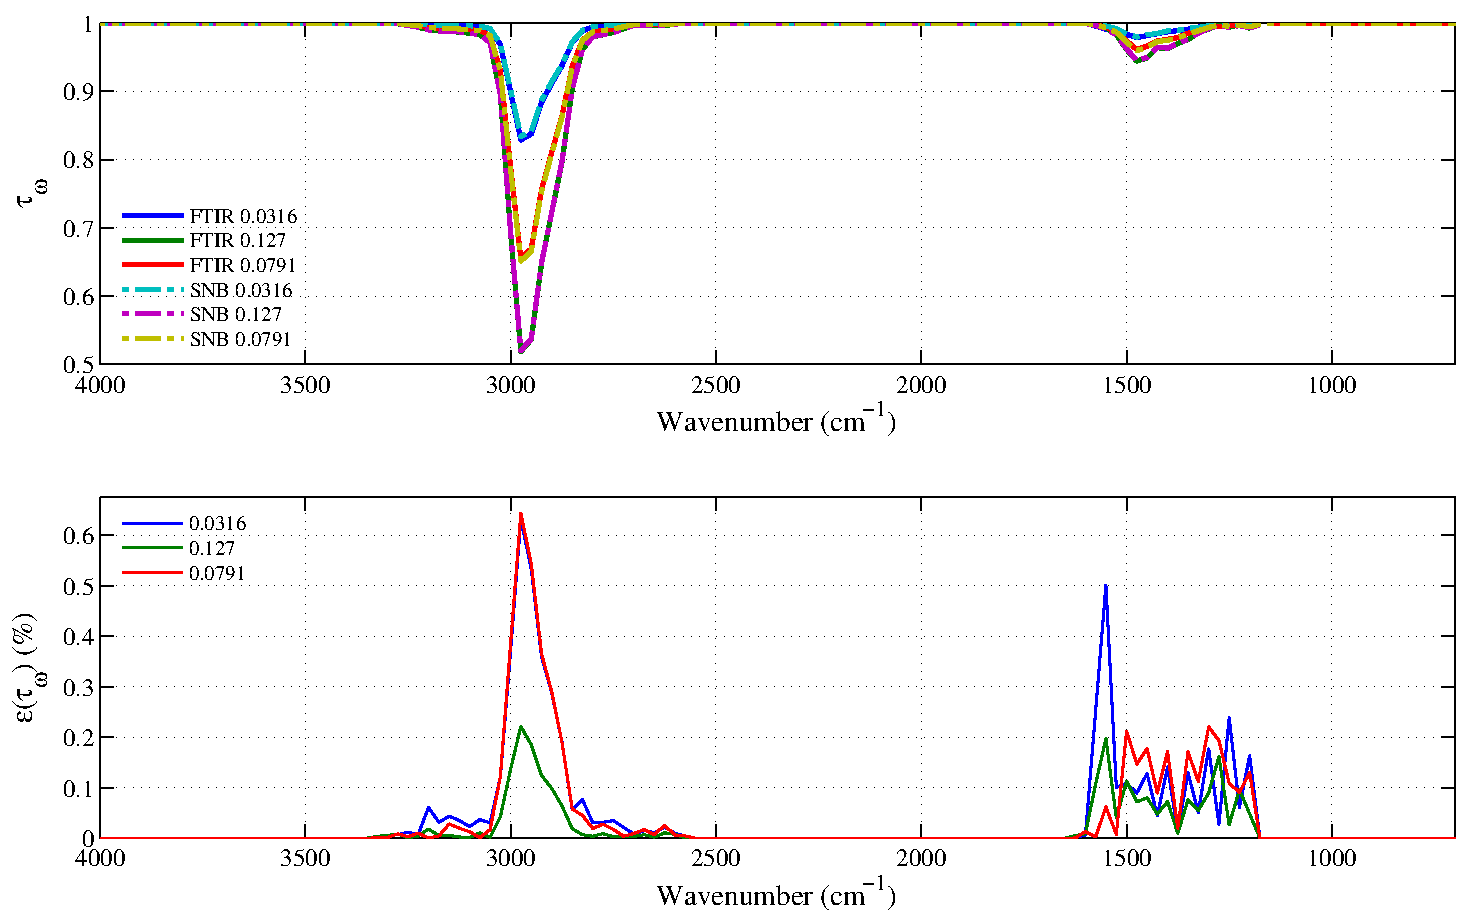
\includegraphics[width=\textwidth]{Figures/Comparison_Fit_Propane_MALKMUS_Temp513K.pdf}
\caption{Top: comparison between the experimental (FTIR, in solid lines) and the synthetic (dashed lines) spectral transmissivity profiles, denoted $\tau_{\omega}$, of an isothermal homogeneous column of propane. The synthetic profiles was generated using the Malkmus narrow band parameters presented in Figs.~\ref{fig:propane_kappa_beta1} to \ref{fig:propane_kappa_beta2}. Bottom: relative transmissivity error, denoted $\epsilon{(\tau_{\omega})}$, between the experiment and the synthetic profiles presented on the top figure. Three different pressure-paths are considered: 0.127, 0.0791 and 0.0316 atm.cm. The gas temperature is set at 513~K and the total pressure is 101 kPa. Note: the experimental data resolution has been changed to match that of the narrow band model. \label{fig:propane_SNBVerify_513K}}
\end{figure}

\begin{figure}[p]
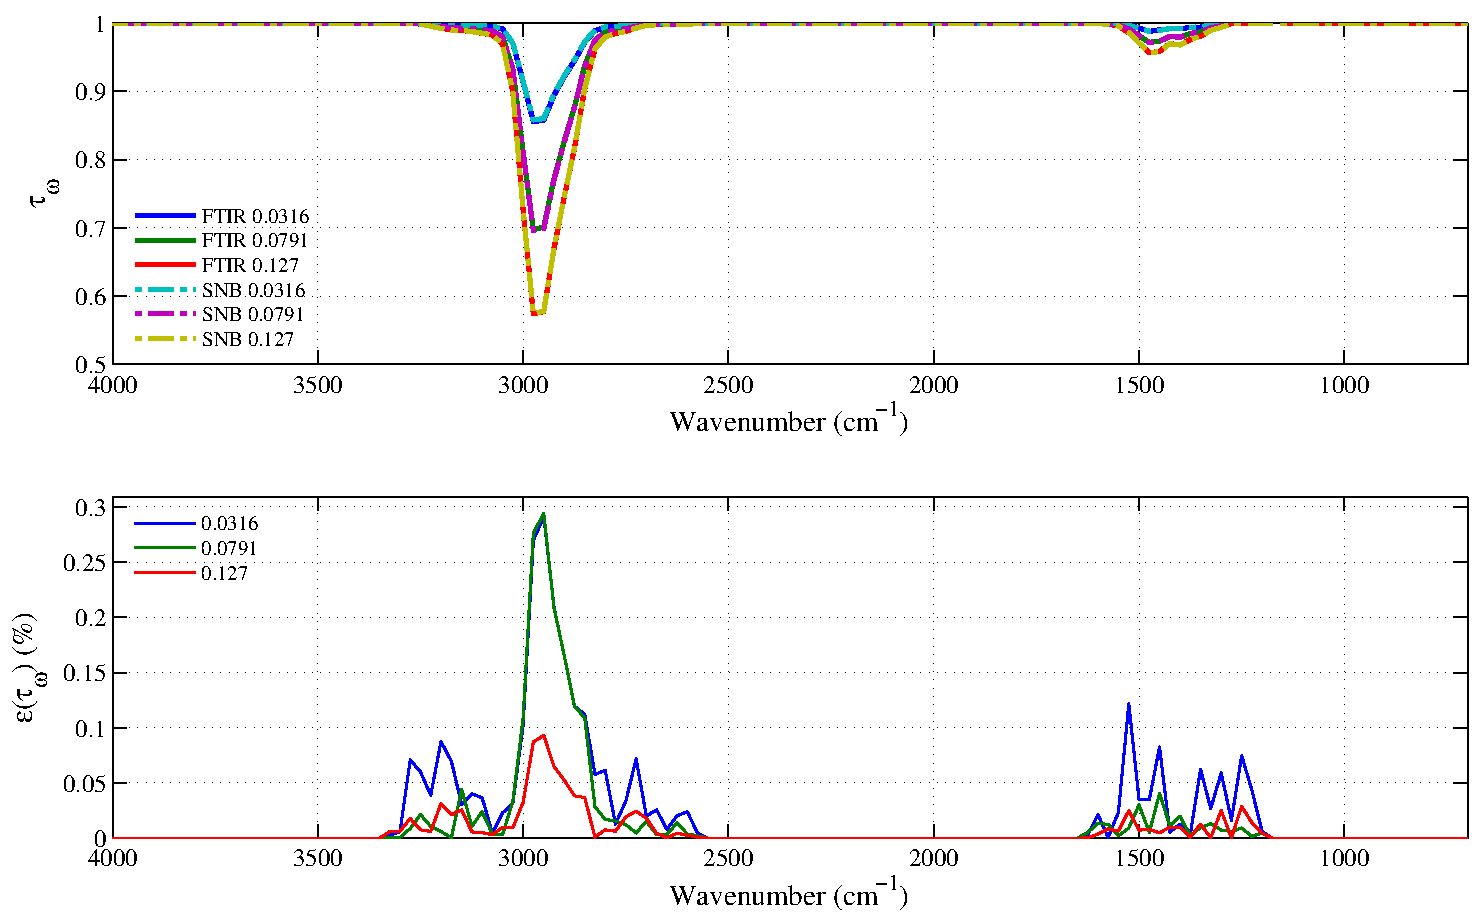
\includegraphics[width=\textwidth]{Figures/Comparison_Fit_Propane_MALKMUS_Temp578K.pdf}
\caption{Top: comparison between the experimental (FTIR, in solid lines) and the synthetic (dashed lines) spectral transmissivity profiles, denoted $\tau_{\omega}$, of an isothermal homogeneous column of propane. The synthetic profiles was generated using the Malkmus narrow band parameters presented in Figs.~\ref{fig:propane_kappa_beta1} to \ref{fig:propane_kappa_beta2}. Bottom: relative transmissivity error, denoted $\epsilon{(\tau_{\omega})}$, between the experiment and the synthetic profiles presented on the top figure. Three different pressure-paths are considered: 0.127, 0.0791 and 0.0316 atm.cm. The gas temperature is set at 578~K and the total pressure is 101 kPa. Note: the experimental data resolution has been changed to match that of the narrow band model. \label{fig:propane_SNBVerify_578K}}
\end{figure}

\begin{figure}[p]
\includegraphics[width=\textwidth]{Figures/Comparison_Fit_Propane_MALKMUS_Temp790K.pdf}
\caption{Top: comparison between the experimental (FTIR, in solid lines) and the synthetic (dashed lines) spectral transmissivity profiles, denoted $\tau_{\omega}$, of an isothermal homogeneous column of propane. The synthetic profiles was generated using the Malkmus narrow band parameters presented in Figs.~\ref{fig:propane_kappa_beta1} to \ref{fig:propane_kappa_beta2}. Bottom: relative transmissivity error, denoted $\epsilon{(\tau_{\omega})}$, between the experiment and the synthetic profiles presented on the top figure. Three different pressure-paths are considered: 0.127, 0.0791 and 0.0316 atm.cm. The gas temperature is set at 790~K and the total pressure is 101 kPa. Note: the experimental data resolution has been changed to match that of the narrow band model. \label{fig:propane_SNBVerify_790K}}
\end{figure}

\begin{figure}[p]
\includegraphics[width=\textwidth]{Figures/Comparison_Fit_Propane_MALKMUS_Temp1009K.pdf}
\caption{Top: comparison between the experimental (FTIR, in solid lines) and the synthetic (dashed lines) spectral transmissivity profiles, denoted $\tau_{\omega}$, of an isothermal homogeneous column of propane. The synthetic profiles was generated using the Malkmus narrow band parameters presented in Figs.~\ref{fig:propane_kappa_beta1} to \ref{fig:propane_kappa_beta2}. Bottom: relative transmissivity error, denoted $\epsilon{(\tau_{\omega})}$, between the experiment and the synthetic profiles presented on the top figure. Three different pressure-paths are considered: 0.127, 0.0791 and 0.0316 atm.cm. The gas temperature is set at 1009~K and the total pressure is 101 kPa. Note: the experimental data resolution has been changed to match that of the narrow band model. \label{fig:propane_SNBVerify_1009K}}
\end{figure}


\clearpage

\section{Toluene: $\rm C_7H_8$}

\subsection{Integrated Band Intensity}

Toluene, $\rm C_7H_8$, has only one plane of symmetry; it belongs to the point group $C_{s}$~\cite{Herzberg1949}. Its IR spectrum is the result of the vibration-rotation modes of the $\rm C=C$, $\rm CH$, and $\rm CH_3$ groups. It has 39 vibrational modes. In RadCal, its IR spectrum has been divided into five distinct bands. The first band from 700--805~cm$\rm^{-1}$ is associated with the bending motion of the $\rm CH$ chemical group. The second band from 975--1175~cm$\rm^{-1}$ is associated with the bending motion of the $\rm CH$ chemical group. The third band from 1275--1650~cm$\rm^{-1}$ is associated with the bending motion of the $\rm CH_3$ chemical group. The fourth band from 1650--2075~cm$\rm^{-1}$ is associated with the stretching motion of the $\rm C=C$ chemical group. The fifth band from 2675--3225~cm$\rm^{-1}$ is associated with the stretching motion of the $\rm CH_3$ and $\rm CH$ chemical groups. The first and fifth bands have the highest integrated band intensity. See Table \ref{Table::C7H8}.
\begin{table}[ht]
   \centering
   \caption{Spectral bands of $\rm C_7H_8$ included in RadCal.}
   \vspace{0.1in}
   \label{Table::C7H8}
   \begin{tabular}{|c|c|c|c|c|}
    \hline
    Band \# & \multicolumn{2}{|l|}{Bounds (cm$\rm ^{-1}$) } & Assignment & $\alpha(T=300 \; {\rm K}) \; (\rm {atm^{-1} cm^{-2}})$\\
    \cline{1-5}
    1 & 700  & 805  &  $\rm CH$ Bending      & 234 \\
    2 & 975  & 1175 &  $\rm CH$ Bending      & 40  \\
    3 & 1275 & 1650 &  $\rm CH_3$ Bending    & 166 \\
    4 & 1650 & 2075 &  $\rm C=C$ Stretching  & 205 \\
    5 & 2675 & 3225 &  $\rm CH_3$, $\rm CH$  Stretching & 507  \\
    \hline
   \end{tabular}
\end{table}

\subsection{Malkmus Narrow Band Parameters}

All the toluene IR spectral absorption data were obtained from high resolution FTIR experiments with temperatures varying from 300~K to 999~K. The spectral absorption coefficients were obtained by fitting the experimental spectral transmissivity of a homogeneous column of isothermal toluene with a total pressure of 1~atm using the Malkmus model.

The toluene narrow band parameters, $\bar{\kappa}$ and $\beta$, for temperatures ranging from 300~K to 999~K are plotted in Figures~\ref{fig:toluene_kappa_beta1}--\ref{fig:toluene_kappa_beta5} for Bands 1 to 5.

\newpage

\begin{figure}[p]
\begin{center}
\includegraphics[width=5.0in]{Figures/Toluene_Kappa_Band1_MALKMUS.pdf}
\includegraphics[width=5.0in]{Figures/Toluene_Beta_Band1_MALKMUS.pdf}
\end{center}
\caption{Toluene narrow band parameters $\bar{\kappa}$ and $\beta$ obtained for the 700--805~cm$^{-1}$ band corresponding to the bending motion of the $\rm CH$ chemical group. Temperatures plotted are: 300, 396, 440, 477, 587, 795, and 999~K. The narrow band resolution $\Delta \om$ is 5~cm$^{-1}$.\label{fig:toluene_kappa_beta1}}
\end{figure}

\begin{figure}[p]
\begin{center}
\includegraphics[width=5.0in]{Figures/Toluene_Kappa_Band2_MALKMUS.pdf}
\includegraphics[width=5.0in]{Figures/Toluene_Beta_Band2_MALKMUS.pdf}
\end{center}
\caption{Toluene narrow band parameters $\bar{\kappa}$ and $\beta$ obtained for the 975--1175~cm$^{-1}$ band corresponding to the bending motion of the $\rm CH$ chemical group. Temperatures plotted are: 300, 396, 440, 477, 587, 795, and 999~K. The narrow band resolution $\Delta \om$ is 5~cm$^{-1}$.\label{fig:toluene_kappa_beta2}}
\end{figure}

\begin{figure}[p]
\begin{center}
\includegraphics[width=5.0in]{Figures/Toluene_Kappa_Band3_MALKMUS.pdf}
\includegraphics[width=5.0in]{Figures/Toluene_Beta_Band3_MALKMUS.pdf}
\end{center}
\caption{Toluene narrow band parameters $\bar{\kappa}$ and $\beta$ obtained for the 1275--1650~cm$^{-1}$ band corresponding to the bending motion of the $\rm CH_3$ chemical group. Temperatures plotted are: 300, 396, 440, 477, 587, 795, and 999~K. The narrow band resolution $\Delta \om$ is 25~cm$^{-1}$.\label{fig:toluene_kappa_beta3}}
\end{figure}

\begin{figure}[p]
\begin{center}
\includegraphics[width=5.0in]{Figures/Toluene_Kappa_Band4_MALKMUS.pdf}
\includegraphics[width=5.0in]{Figures/Toluene_Beta_Band4_MALKMUS.pdf}
\end{center}
\caption{Toluene narrow band parameters $\bar{\kappa}$ and $\beta$ obtained for the 1650--2075~cm$^{-1}$ band corresponding to the stretching motion of the $\rm C=C$ chemical group. Temperatures plotted are: 300, 396, 440, 477, 587, 795, and 999~K. The narrow band resolution $\Delta \om$ is 25~cm$^{-1}$.\label{fig:toluene_kappa_beta4}}
\end{figure}

\begin{figure}[p]
\begin{center}
\includegraphics[width=5.0in]{Figures/Toluene_Kappa_Band5_MALKMUS.pdf}
\includegraphics[width=5.0in]{Figures/Toluene_Beta_Band5_MALKMUS.pdf}
\end{center}
\caption{Toluene narrow band parameters $\bar{\kappa}$ and $\beta$ obtained for the 2675--3225~cm$^{-1}$ band corresponding to the bending motion of the $\rm CH_3$ and $\rm CH$ chemical groups. Temperatures plotted are: 300, 396, 440, 477, 587, 795, and 999~K. The narrow band resolution $\Delta \om$ is 25~cm$^{-1}$.\label{fig:toluene_kappa_beta5}}
\end{figure}

\FloatBarrier

\subsection{Verification SNB Parameters}

To assess the accuracy of the narrow band parameters $\bar{\kappa}$ and $\beta$, synthetic transmissivities were constructed for the same experimental conditions as the FTIR data and compare with it. This subsection plots the comparison and the relative error in transmissivity (relative to FTIR measurements) using the toluene parameters presented in Figs.~\ref{fig:toluene_kappa_beta1} to \ref{fig:toluene_kappa_beta5}.

\begin{figure}[!h]
\includegraphics[width=\textwidth]{Figures/Comparison_Fit_Toluene_MALKMUS_Temp300K.pdf}
\caption{Top: comparison between the experimental (FTIR, in solid lines) and the synthetic (dashed lines) spectral transmissivity profiles, denoted $\tau_{\omega}$, of an isothermal homogeneous column of toluene. The synthetic profiles was generated using the Malkmus narrow band parameters presented in Figs.~\ref{fig:toluene_kappa_beta1} to \ref{fig:toluene_kappa_beta5}. Bottom: relative transmissivity error, denoted $\epsilon{(\tau_{\omega})}$, between the experiment and the synthetic profiles presented on the top figure. Three different pressure-paths are considered: 0.135, 0.101 and 0.0806 atm.cm. The gas temperature is set at 300~K and the total pressure is 101 kPa. Note: the experimental data resolution has been changed to match that of the narrow band model. \label{fig:toluene_SNBVerify_300K}}
\end{figure}

\begin{figure}[p]
\includegraphics[width=\textwidth]{Figures/Comparison_Fit_Toluene_MALKMUS_Temp396K.pdf}
\caption{Top: comparison between the experimental (FTIR, in solid lines) and the synthetic (dashed lines) spectral transmissivity profiles, denoted $\tau_{\omega}$, of an isothermal homogeneous column of toluene. The synthetic profiles was generated using the Malkmus narrow band parameters presented in Figs.~\ref{fig:toluene_kappa_beta1} to \ref{fig:toluene_kappa_beta5}. Bottom: relative transmissivity error, denoted $\epsilon{(\tau_{\omega})}$, between the experiment and the synthetic profiles presented on the top figure. Three different pressure-paths are considered: 0.124, 0.0956 and 0.0808 atm.cm. The gas temperature is set at 396~K and the total pressure is 101 kPa. Note: the experimental data resolution has been changed to match that of the narrow band model. \label{fig:toluene_SNBVerify_396K}}
\end{figure}

\begin{figure}[p]
\includegraphics[width=\textwidth]{Figures/Comparison_Fit_Toluene_MALKMUS_Temp440K.pdf}
\caption{Top: comparison between the experimental (FTIR, in solid lines) and the synthetic (dashed lines) spectral transmissivity profiles, denoted $\tau_{\omega}$, of an isothermal homogeneous column of toluene. The synthetic profiles was generated using the Malkmus narrow band parameters presented in Figs.~\ref{fig:toluene_kappa_beta1} to \ref{fig:toluene_kappa_beta5}. Bottom: relative transmissivity error, denoted $\epsilon{(\tau_{\omega})}$, between the experiment and the synthetic profiles presented on the top figure. Three different pressure-paths are considered:0.109, 0.0844 and 0.0741. The gas temperature is set at 440~K and the total pressure is 101 kPa. Note: the experimental data resolution has been changed to match that of the narrow band model. \label{fig:toluene_SNBVerify_440K}}
\end{figure}

\begin{figure}[p]
\includegraphics[width=\textwidth]{Figures/Comparison_Fit_Toluene_MALKMUS_Temp477K.pdf}
\caption{Top: comparison between the experimental (FTIR, in solid lines) and the synthetic (dashed lines) spectral transmissivity profiles, denoted $\tau_{\omega}$, of an isothermal homogeneous column of toluene. The synthetic profiles was generated using the Malkmus narrow band parameters presented in Figs.~\ref{fig:toluene_kappa_beta1} to \ref{fig:toluene_kappa_beta5}. Bottom: relative transmissivity error, denoted $\epsilon{(\tau_{\omega})}$, between the experiment and the synthetic profiles presented on the top figure. Three different pressure-paths are considered: 0.125, 0.096 and 0.0828 atm.cm. The gas temperature is set at 477~K and the total pressure is 101 kPa. Note: the experimental data resolution has been changed to match that of the narrow band model. \label{fig:toluene_SNBVerify_477K}}
\end{figure}

\begin{figure}[p]
\includegraphics[width=\textwidth]{Figures/Comparison_Fit_Toluene_MALKMUS_Temp587K.pdf}
\caption{Top: comparison between the experimental (FTIR, in solid lines) and the synthetic (dashed lines) spectral transmissivity profiles, denoted $\tau_{\omega}$, of an isothermal homogeneous column of toluene. The synthetic profiles was generated using the Malkmus narrow band parameters presented in Figs.~\ref{fig:toluene_kappa_beta1} to \ref{fig:toluene_kappa_beta5}. Bottom: relative transmissivity error, denoted $\epsilon{(\tau_{\omega})}$, between the experiment and the synthetic profiles presented on the top figure. Three different pressure-paths are considered: 0.118, 0.0958 and 0.0809 atm.cm. The gas temperature is set at 587~K and the total pressure is 101 kPa. Note: the experimental data resolution has been changed to match that of the narrow band model. \label{fig:toluene_SNBVerify_587K}}
\end{figure}

\begin{figure}[p]
\includegraphics[width=\textwidth]{Figures/Comparison_Fit_Toluene_MALKMUS_Temp795K.pdf}
\caption{Top: comparison between the experimental (FTIR, in solid lines) and the synthetic (dashed lines) spectral transmissivity profiles, denoted $\tau_{\omega}$, of an isothermal homogeneous column of toluene. The synthetic profiles was generated using the Malkmus narrow band parameters presented in Figs.~\ref{fig:toluene_kappa_beta1} to \ref{fig:toluene_kappa_beta5}. Bottom: relative transmissivity error, denoted $\epsilon{(\tau_{\omega})}$, between the experiment and the synthetic profiles presented on the top figure. Three different pressure-paths are considered: 0.127, 0.0963 and 0.0831 atm.cm. The gas temperature is set at 795~K and the total pressure is 101 kPa. Note: the experimental data resolution has been changed to match that of the narrow band model. \label{fig:toluene_SNBVerify_795K}}
\end{figure}


\begin{figure}[p]
\includegraphics[width=\textwidth]{Figures/Comparison_Fit_Toluene_MALKMUS_Temp999K.pdf}
\caption{Top: comparison between the experimental (FTIR, in solid lines) and the synthetic (dashed lines) spectral transmissivity profiles, denoted $\tau_{\omega}$, of an isothermal homogeneous column of toluene. The synthetic profiles was generated using the Malkmus narrow band parameters presented in Figs.~\ref{fig:toluene_kappa_beta1} to \ref{fig:toluene_kappa_beta5}. Bottom: relative transmissivity error, denoted $\epsilon{(\tau_{\omega})}$, between the experiment and the synthetic profiles presented on the top figure. Three different pressure-paths are considered: 0.138, 0.103 and 0.0893 atm.cm. The gas temperature is set at 999~K and the total pressure is 101 kPa. Note: the experimental data resolution has been changed to match that of the narrow band model. \label{fig:toluene_SNBVerify_999K}}
\end{figure}


\clearpage

\section{\textit{n}-Heptane: $\rm C_7H_{16}$}

\subsection{Integrated Band Intensity}

\textit{n}-heptane, $\rm C_7H_16$, has two planes of symmetry and two axes of rotation. It belongs to the point group $C_{2v}$~\cite{Herzberg1949}. The \textit{n}-heptane IR spectrum results from the vibration-rotation modes of the $\rm C-C$, $\rm CH_2$, and $\rm CH_3$ groups. It has 63 vibrational modes. In RadCal, its IR spectrum has been divided into two distinct bands. The first band from 1100--1800~cm$\rm^{-1}$ is associated with the bending motion of the $\rm CH_2$ and $\rm CH_3$ chemical groups. The second band from 2250--3275~cm$\rm^{-1}$ is associated with the stretching motion of the $\rm CH_2$ and $\rm CH_3$ chemical groups. This band has the highest integrated band intensity. Its value is more than 10 times that of the first band, see Table \ref{Table::C7H16}.
\begin{table}[ht]
   \centering
   \caption{Spectral bands of $\rm C_7H_{16}$ included in RadCal.}
   \vspace{0.1in}
   \label{Table::C7H16}
   \begin{tabular}{|c|c|c|c|c|}
    \hline
    Band \# & \multicolumn{2}{|l|}{Bounds (cm$\rm ^{-1}$) } & Assignment & $\alpha(T=293 \; {\rm K}) \; (\rm {atm^{-1} cm^{-2}})$\\
    \cline{1-5}
    1 & 1100  & 1800 &  $\rm CH_2, CH_3$ Bending    & 304 \\
    2 & 2250  & 3275 &  $\rm CH_2, CH_3$ Stretching & 3165 \\
    \hline
   \end{tabular}
\end{table}

\subsection{Malkmus Narrow Band Parameters}

All the \textit{n}-heptane IR spectral absorption data were obtained from high resolution FTIR experiments with temperatures varying from 293~K to 794~K. The spectral absorption coefficients were obtained by fitting the experimental spectral transmissivity of a homogeneous column of isothermal \textit{n}-heptane with a total pressure of 1~atm using the Malkmus model.

The \textit{n}-heptane narrow band parameters, $\bar{\kappa}$ and $\beta$, for temperatures ranging from 293~K to 1000~K are plotted in Figures~\ref{fig:nheptane_kappa_beta1}--\ref{fig:nheptane_kappa_beta2} for Bands 1 and 2.

\newpage

\begin{figure}[p]
\begin{center}
\includegraphics[width=5.0in]{Figures/Heptane_Kappa_Band1_MALKMUS.pdf}
\includegraphics[width=5.0in]{Figures/Heptane_Beta_Band1_MALKMUS.pdf}
\end{center}
\caption{\textit{n}-heptane narrow band parameters $\bar{\kappa}$ and $\beta$ obtained for the 1100--1800~cm$^{-1}$ band corresponding to the bending motion of the $\rm CH_2$ and $\rm CH_3$ chemical groups. Temperatures plotted are: 293, 400, 450, 490, 593, 794, and 1000~K. The narrow band resolution $\Delta \om$ is 25~cm$^{-1}$.\label{fig:nheptane_kappa_beta1}}
\end{figure}

\begin{figure}[p]
\begin{center}
\includegraphics[width=5.0in]{Figures/Heptane_Kappa_Band2_MALKMUS.pdf}
\includegraphics[width=5.0in]{Figures/Heptane_Beta_Band2_MALKMUS.pdf}
\end{center}
\caption{\textit{n}-heptane narrow band parameters $\bar{\kappa}$ and $\beta$ obtained for the 2250--3275~cm$^{-1}$ band corresponding to the stretching motion of the $\rm CH_2$ and $\rm CH_3$ chemical groups. Temperatures plotted are: 293, 400, 450, 490, 593, 794, and 1000~K. The narrow band resolution $\Delta \om$ is 25~cm$^{-1}$.\label{fig:nheptane_kappa_beta2}}
\end{figure}

\FloatBarrier

\subsection{Verification SNB Parameters}

To assess the accuracy of the narrow band parameters $\bar{\kappa}$ and $\beta$, synthetic transmissivities were constructed for the same experimental conditions as the FTIR data and compare with it. This subsection plots the comparison and the relative error in transmissivity (relative to FTIR measurements) using the \textit{n}-heptane parameters presented in Figs.~\ref{fig:nheptane_kappa_beta1} to \ref{fig:nheptane_kappa_beta2}.

\begin{figure}[!h]
\includegraphics[width=\textwidth]{Figures/Comparison_Fit_Heptane_MALKMUS_Temp293K.pdf}
\caption{Top: comparison between the experimental (FTIR, in solid lines) and the synthetic (dashed lines) spectral transmissivity profiles, denoted $\tau_{\omega}$, of an isothermal homogeneous column of \textit{n}-heptane. The synthetic profiles was generated using the Malkmus narrow band parameters presented in Figs.~\ref{fig:nheptane_kappa_beta1} to \ref{fig:nheptane_kappa_beta2}. Bottom: relative transmissivity error, denoted $\epsilon{(\tau_{\omega})}$, between the experiment and the synthetic profiles presented on the top figure. Three different pressure-paths are considered: 0.0492, 0.0312 and 0.015 atm.cm. The gas temperature is set at 293~K and the total pressure is 101 kPa. Note: the experimental data resolution has been changed to match that of the narrow band model. \label{fig:nheptane_SNBVerify_293K}}
\end{figure}

\begin{figure}[p]
\includegraphics[width=\textwidth]{Figures/Comparison_Fit_Heptane_MALKMUS_Temp400K.pdf}
\caption{Top: comparison between the experimental (FTIR, in solid lines) and the synthetic (dashed lines) spectral transmissivity profiles, denoted $\tau_{\omega}$, of an isothermal homogeneous column of \textit{n}-heptane. The synthetic profiles was generated using the Malkmus narrow band parameters presented in Figs.~\ref{fig:nheptane_kappa_beta1} to \ref{fig:nheptane_kappa_beta2}. Bottom: relative transmissivity error, denoted $\epsilon{(\tau_{\omega})}$, between the experiment and the synthetic profiles presented on the top figure. Three different pressure-paths are considered: 0.0475, 0.0301 and 0.0145 atm.cm. The gas temperature is set at 400~K and the total pressure is 101 kPa. Note: the experimental data resolution has been changed to match that of the narrow band model. \label{fig:nheptane_SNBVerify_400K}}
\end{figure}

\begin{figure}[p]
\includegraphics[width=\textwidth]{Figures/Comparison_Fit_Heptane_MALKMUS_Temp450K.pdf}
\caption{Top: comparison between the experimental (FTIR, in solid lines) and the synthetic (dashed lines) spectral transmissivity profiles, denoted $\tau_{\omega}$, of an isothermal homogeneous column of \textit{n}-heptane. The synthetic profiles was generated using the Malkmus narrow band parameters presented in Figs.~\ref{fig:nheptane_kappa_beta1} to \ref{fig:nheptane_kappa_beta2}. Bottom: relative transmissivity error, denoted $\epsilon{(\tau_{\omega})}$, between the experiment and the synthetic profiles presented on the top figure. Three different pressure-paths are considered:0.0495, 0.0311 and 0.0152. The gas temperature is set at 450~K and the total pressure is 101 kPa. Note: the experimental data resolution has been changed to match that of the narrow band model. \label{fig:nheptane_SNBVerify_450K}}
\end{figure}

\begin{figure}[p]
\includegraphics[width=\textwidth]{Figures/Comparison_Fit_Heptane_MALKMUS_Temp490K.pdf}
\caption{Top: comparison between the experimental (FTIR, in solid lines) and the synthetic (dashed lines) spectral transmissivity profiles, denoted $\tau_{\omega}$, of an isothermal homogeneous column of \textit{n}-heptane. The synthetic profiles was generated using the Malkmus narrow band parameters presented in Figs.~\ref{fig:nheptane_kappa_beta1} to \ref{fig:nheptane_kappa_beta2}. Bottom: relative transmissivity error, denoted $\epsilon{(\tau_{\omega})}$, between the experiment and the synthetic profiles presented on the top figure. Three different pressure-paths are considered: 0.0494, 0.0305 and 0.015 atm.cm. The gas temperature is set at 490~K and the total pressure is 101 kPa. Note: the experimental data resolution has been changed to match that of the narrow band model. \label{fig:nheptane_SNBVerify_490K}}
\end{figure}

\begin{figure}[p]
\includegraphics[width=\textwidth]{Figures/Comparison_Fit_Heptane_MALKMUS_Temp593K.pdf}
\caption{Top: comparison between the experimental (FTIR, in solid lines) and the synthetic (dashed lines) spectral transmissivity profiles, denoted $\tau_{\omega}$, of an isothermal homogeneous column of \textit{n}-heptane. The synthetic profiles was generated using the Malkmus narrow band parameters presented in Figs.~\ref{fig:nheptane_kappa_beta1} to \ref{fig:nheptane_kappa_beta2}. Bottom: relative transmissivity error, denoted $\epsilon{(\tau_{\omega})}$, between the experiment and the synthetic profiles presented on the top figure. Three different pressure-paths are considered: 0.0503, 0.0314 and 0.0152 atm.cm. The gas temperature is set at 593~K and the total pressure is 101 kPa. Note: the experimental data resolution has been changed to match that of the narrow band model. \label{fig:nheptane_SNBVerify_593K}}
\end{figure}

\begin{figure}[p]
\includegraphics[width=\textwidth]{Figures/Comparison_Fit_Heptane_MALKMUS_Temp794K.pdf}
\caption{Top: comparison between the experimental (FTIR, in solid lines) and the synthetic (dashed lines) spectral transmissivity profiles, denoted $\tau_{\omega}$, of an isothermal homogeneous column of \textit{n}-heptane. The synthetic profiles was generated using the Malkmus narrow band parameters presented in Figs.~\ref{fig:nheptane_kappa_beta1} to \ref{fig:nheptane_kappa_beta2}. Bottom: relative transmissivity error, denoted $\epsilon{(\tau_{\omega})}$, between the experiment and the synthetic profiles presented on the top figure. Three different pressure-paths are considered: 0.044, 0.0301, and 0.0148 atm.cm. The gas temperature is set at 794~K and the total pressure is 101 kPa. Note: the experimental data resolution has been changed to match that of the narrow band model. \label{fig:nheptane_SNBVerify_794K}}
\end{figure}

\begin{figure}[p]
\includegraphics[width=\textwidth]{Figures/Comparison_Fit_Heptane_MALKMUS_Temp1000K.pdf}
\caption{Top: comparison between the experimental (FTIR, in solid lines) and the synthetic (dashed lines) spectral transmissivity profiles, denoted $\tau_{\omega}$, of an isothermal homogeneous column of \textit{n}-heptane. The synthetic profiles was generated using the Malkmus narrow band parameters presented in Figs.~\ref{fig:nheptane_kappa_beta1} to \ref{fig:nheptane_kappa_beta2}. Bottom: relative transmissivity error, denoted $\epsilon{(\tau_{\omega})}$, between the experiment and the synthetic profiles presented on the top figure. Three different pressure-paths are considered: 0.0364, 0.0307 and 0.0173 atm.cm. The gas temperature is set at 1000~K and the total pressure is 101 kPa. Note: the experimental data resolution has been changed to match that of the narrow band model. \label{fig:nheptane_SNBVerify_1000K}}
\end{figure}


\clearpage

\section{Methanol: $\rm CH_3OH$}

\subsection{Integrated Band Intensity}

Methanol, $\rm CH_3OH$, has only one plane of symmetry. It belongs to the point group $C_{s}$~\cite{Herzberg1949}. Its IR spectrum results from the vibration-rotation modes of the $\rm C-O$, $\rm OH$, and $\rm CH_3$ groups. It has 12 vibrational modes. In RadCal, its IR spectrum has been divided into four distinct bands. The first band from 825--1125~cm$\rm^{-1}$ is associated with the stretching motion of the $\rm C-O$ chemical group. The second band from 1125--1700~cm$^{-1}$ is associated with the bending motion of the $\rm CH_3$ and $\rm OH$ chemical groups. The third band from 2600--3225~cm$\rm^{-1}$ is associated with the stretching motion of the $\rm CH_3$ chemical group. The fourth and last band from 3525--3850~cm$\rm^{-1}$ is associated with the stretching motion of the $\rm OH$ chemical group. The strongest absorbing bands are the third band (2600--3225~cm$\rm^{-1}$) and the first band (825--1125~cm$\rm^{-1}$). See Table \ref{Table::CH3OH}.
\begin{table}[ht]
   \centering
   \caption{Spectral bands of $\rm CH_3OH$ included in RadCal.}
   \vspace{0.1in}
   \label{Table::CH3OH}
   \begin{tabular}{|c|c|c|c|c|}
    \hline
    Band \# & \multicolumn{2}{|l|}{Bounds (cm$\rm ^{-1}$) } & Assignment &  $\alpha(T=293 \; {\rm K}) \; (\rm {atm^{-1} cm^{-2}})$ \\
    \cline{1-5}
    1 & 825  & 1125 & $\rm C-O$ Stretching   & 598 \\
    2 & 1125 & 1700 & $\rm CH_3, OH$ Bending & 199 \\
    3 & 2600 & 3225 & $\rm CH_3$ Stretching  & 680 \\
    4 & 3525 & 3850 & $\rm OH$ Stretching    & 112 \\
    \hline
   \end{tabular}
\end{table}

\subsection{Malkmus Narrow Band Parameters}

All the methanol IR spectral absorption data were obtained from high resolution FTIR experiments with temperatures varying from 293~K to 804~K. The spectral absorption coefficients were obtained by fitting the experimental spectral transmissivity of a homogeneous column of isothermal methanol with a total pressure of 1~atm using the Malkmus model.

The methanol narrow band parameters, $\bar{\kappa}$ and $\beta$, for temperatures ranging from 293~K to 1000~K are plotted in Figures~\ref{fig:methanol_kappa_beta1}--\ref{fig:methanol_kappa_beta4} for Bands 1 to 4.

\newpage

\begin{figure}[p]
\begin{center}
\includegraphics[width=5.0in]{Figures/Methanol_Kappa_Band1_MALKMUS.pdf}
\includegraphics[width=5.0in]{Figures/Methanol_Beta_Band1_MALKMUS.pdf}
\end{center}
\caption{Methanol narrow band parameters $\bar{\kappa}$ and $\beta$ obtained for the 825--1125~cm$^{-1}$ band corresponding to the stretching motion of the $\rm C-O$ chemical group. Temperatures plotted are: 293, 396, 443, 483, 570, 804, and 1000~K. The narrow band resolution $\Delta \om$ is 5~cm$^{-1}$.\label{fig:methanol_kappa_beta1}}
\end{figure}

\begin{figure}[p]
\begin{center}
\includegraphics[width=5.0in]{Figures/Methanol_Kappa_Band2_MALKMUS.pdf}
\includegraphics[width=5.0in]{Figures/Methanol_Beta_Band2_MALKMUS.pdf}
\end{center}
\caption{Methanol narrow band parameters $\bar{\kappa}$ and $\beta$ obtained for the 1125--1700~cm$^{-1}$ band corresponding to the bending motion of the $\rm CH_3$ and $\rm OH$ chemical groups. Temperatures plotted are: 293, 396, 443, 483, 570, 804, and 1000~K. The narrow band resolution $\Delta \om$ is 25~cm$^{-1}$.\label{fig:methanol_kappa_beta2}}
\end{figure}

\begin{figure}[p]
\begin{center}
\includegraphics[width=5.0in]{Figures/Methanol_Kappa_Band3_MALKMUS.pdf}
\includegraphics[width=5.0in]{Figures/Methanol_Beta_Band3_MALKMUS.pdf}
\end{center}
\caption{Methanol narrow band parameters $\bar{\kappa}$ and $\beta$ obtained for the 2600--3225~cm$^{-1}$ band corresponding to the stretching motion of the $\rm CH_3$ chemical groups. Temperatures plotted are: 293, 396, 443, 483, 570, 804, and 1000~K. The narrow band resolution $\Delta \om$ is 25~cm$^{-1}$.\label{fig:methanol_kappa_beta3}}
\end{figure}

\begin{figure}[p]
\begin{center}
\includegraphics[width=5.0in]{Figures/Methanol_Kappa_Band4_MALKMUS.pdf}
\includegraphics[width=5.0in]{Figures/Methanol_Beta_Band4_MALKMUS.pdf}
\end{center}
 \caption{Methanol narrow band parameters $\bar{\kappa}$ and $\beta$ obtained for the 3525--3850~cm$^{-1}$ band corresponding to the stretching motion of the $\rm OH$ chemical groups. Temperatures plotted are: 293, 396, 443, 483, 570, 804, and 1000~K. The narrow band resolution $\Delta \om$ is 25~cm$^{-1}$.\label{fig:methanol_kappa_beta4}}
\end{figure}

\FloatBarrier

\subsection{Verification SNB Parameters}

To assess the accuracy of the narrow band parameters $\bar{\kappa}$ and $\beta$, synthetic transmissivities were constructed for the same experimental conditions as the FTIR data and compare with it. This subsection plots the comparison and the relative error in transmissivity (relative to FTIR measurements) using the methanol parameters presented in Figs.~\ref{fig:methanol_kappa_beta1} to \ref{fig:methanol_kappa_beta4}.

\begin{figure}[!h]
\includegraphics[width=\textwidth]{Figures/Comparison_Fit_Methanol_MALKMUS_Temp293K.pdf}
\caption{Top: comparison between the experimental (FTIR, in solid lines) and the synthetic (dashed lines) spectral transmissivity profiles, denoted $\tau_{\omega}$, of an isothermal homogeneous column of methanol. The synthetic profiles was generated using the Malkmus narrow band parameters presented in Figs.~\ref{fig:methanol_kappa_beta1} to \ref{fig:methanol_kappa_beta4}. Bottom: relative transmissivity error, denoted $\epsilon{(\tau_{\omega})}$, between the experiment and the synthetic profiles presented on the top figure. Three different pressure-paths are considered: 0.0922, 0.0714 and 0.0497 atm.cm. The gas temperature is set at 293~K and the total pressure is 101 kPa. Note: the experimental data resolution has been changed to match that of the narrow band model. \label{fig:methanol_SNBVerify_293K}}
\end{figure}

\begin{figure}[p]
\includegraphics[width=\textwidth]{Figures/Comparison_Fit_Methanol_MALKMUS_Temp396K.pdf}
\caption{Top: comparison between the experimental (FTIR, in solid lines) and the synthetic (dashed lines) spectral transmissivity profiles, denoted $\tau_{\omega}$, of an isothermal homogeneous column of methanol. The synthetic profiles was generated using the Malkmus narrow band parameters presented in Figs.~\ref{fig:methanol_kappa_beta1} to \ref{fig:methanol_kappa_beta4}. Bottom: relative transmissivity error, denoted $\epsilon{(\tau_{\omega})}$, between the experiment and the synthetic profiles presented on the top figure. Three different pressure-paths are considered: 0.0929, 0.0735 and 0.0503 atm.cm. The gas temperature is set at 396~K and the total pressure is 101 kPa. Note: the experimental data resolution has been changed to match that of the narrow band model. \label{fig:methanol_SNBVerify_396K}}
\end{figure}

\begin{figure}[p]
\includegraphics[width=\textwidth]{Figures/Comparison_Fit_Methanol_MALKMUS_Temp443K.pdf}
\caption{Top: comparison between the experimental (FTIR, in solid lines) and the synthetic (dashed lines) spectral transmissivity profiles, denoted $\tau_{\omega}$, of an isothermal homogeneous column of methanol. The synthetic profiles was generated using the Malkmus narrow band parameters presented in Figs.~\ref{fig:methanol_kappa_beta1} to \ref{fig:methanol_kappa_beta4}. Bottom: relative transmissivity error, denoted $\epsilon{(\tau_{\omega})}$, between the experiment and the synthetic profiles presented on the top figure. Three different pressure-paths are considered:0.0937, 0.0707 and 0.0457. The gas temperature is set at 443~K and the total pressure is 101 kPa. Note: the experimental data resolution has been changed to match that of the narrow band model. \label{fig:methanol_SNBVerify_443K}}
\end{figure}

\begin{figure}[p]
\includegraphics[width=\textwidth]{Figures/Comparison_Fit_Methanol_MALKMUS_Temp483K.pdf}
\caption{Top: comparison between the experimental (FTIR, in solid lines) and the synthetic (dashed lines) spectral transmissivity profiles, denoted $\tau_{\omega}$, of an isothermal homogeneous column of methanol. The synthetic profiles was generated using the Malkmus narrow band parameters presented in Figs.~\ref{fig:methanol_kappa_beta1} to \ref{fig:methanol_kappa_beta4}. Bottom: relative transmissivity error, denoted $\epsilon{(\tau_{\omega})}$, between the experiment and the synthetic profiles presented on the top figure. Three different pressure-paths are considered: 0.0904, 0.07 and 0.0487 atm.cm. The gas temperature is set at 483~K and the total pressure is 101 kPa. Note: the experimental data resolution has been changed to match that of the narrow band model. \label{fig:methanol_SNBVerify_483K}}
\end{figure}

\begin{figure}[p]
\includegraphics[width=\textwidth]{Figures/Comparison_Fit_Methanol_MALKMUS_Temp570K.pdf}
\caption{Top: comparison between the experimental (FTIR, in solid lines) and the synthetic (dashed lines) spectral transmissivity profiles, denoted $\tau_{\omega}$, of an isothermal homogeneous column of methanol. The synthetic profiles was generated using the Malkmus narrow band parameters presented in Figs.~\ref{fig:methanol_kappa_beta1} to \ref{fig:methanol_kappa_beta4}. Bottom: relative transmissivity error, denoted $\epsilon{(\tau_{\omega})}$, between the experiment and the synthetic profiles presented on the top figure. Three different pressure-paths are considered: 0.0919, 0.0498 and 0.0723 atm.cm. The gas temperature is set at 570~K and the total pressure is 101 kPa. Note: the experimental data resolution has been changed to match that of the narrow band model. \label{fig:methanol_SNBVerify_570K}}
\end{figure}

\begin{figure}[p]
\includegraphics[width=\textwidth]{Figures/Comparison_Fit_Methanol_MALKMUS_Temp804K.pdf}
\caption{Top: comparison between the experimental (FTIR, in solid lines) and the synthetic (dashed lines) spectral transmissivity profiles, denoted $\tau_{\omega}$, of an isothermal homogeneous column of methanol. The synthetic profiles was generated using the Malkmus narrow band parameters presented in Figs.~\ref{fig:methanol_kappa_beta1} to \ref{fig:methanol_kappa_beta4}. Bottom: relative transmissivity error, denoted $\epsilon{(\tau_{\omega})}$, between the experiment and the synthetic profiles presented on the top figure. Three different pressure-paths are considered: 0.101, 0.0782 and 0.0535 atm.cm. The gas temperature is set at 804~K and the total pressure is 101 kPa. Note: the experimental data resolution has been changed to match that of the narrow band model. \label{fig:methanol_SNBVerify_804K}}
\end{figure}

\begin{figure}[p]
\includegraphics[width=\textwidth]{Figures/Comparison_Fit_Methanol_MALKMUS_Temp1000K.pdf}
\caption{Top: comparison between the experimental (FTIR, in solid lines) and the synthetic (dashed lines) spectral transmissivity profiles, denoted $\tau_{\omega}$, of an isothermal homogeneous column of methanol. The synthetic profiles was generated using the Malkmus narrow band parameters presented in Figs.~\ref{fig:methanol_kappa_beta1} to \ref{fig:methanol_kappa_beta4}. Bottom: relative transmissivity error, denoted $\epsilon{(\tau_{\omega})}$, between the experiment and the synthetic profiles presented on the top figure. Three different pressure-paths are considered: 0.0967, 0.0729 and 0.0488 atm.cm. The gas temperature is set at 1000~K and the total pressure is 101 kPa. Note: the experimental data resolution has been changed to match that of the narrow band model. \label{fig:methanol_SNBVerify_1000K}}
\end{figure}


\clearpage

\section{Methyl Methacrylate: $\rm C_5H_8O_2$}

\subsection{Integrated Band Intensity}

Methyl Methacrylate, $\rm C_5H_8O_2$, or MMA, has the most complex IR spectrum of all the fuels presented above. With 15 atoms, it has 39 vibrational modes. The MMA IR spectrum results from the vibration-rotation modes of the $\rm C-O$, $\rm C=O$, $\rm C=C$, $\rm CH_2$, and $\rm CH_3$ groups. In RadCal, its IR spectrum has been divided into six distinct bands. The first band from 750--875~cm$\rm^{-1}$ is associated with the bending motion of the $\rm CH_2$ chemical group. The second band from 875--1050~cm$\rm^{-1}$ is associated with the bending motion of the $\rm CH_2$ chemical group. The third band from 1050--1250~cm$\rm^{-1}$ is associated with the stretching motion of the $\rm C-O$ chemical group. The fourth band from 1250--1550~cm$\rm^{-1}$ is associated with the bending motion of the $\rm CH_3$ chemical group. The fifth band from 1550-1975~cm$\rm^{-1}$ is associated with the stretching motion of the $\rm C=C$ and $\rm C=O$ chemical groups. Finally, the sixth and last band from 2650--3275~cm$\rm^{-1}$ is associated with the stretching motion of the $\rm CH_2$ and $\rm CH_3$ chemical groups. The band with the strongest absorption is the third band (1050--1250~cm$\rm^{-1}$), see Table \ref{Table::C5H8O2}.
\begin{table}[ht]
   \centering
   \caption{Spectral bands of $\rm C_5H_8O_2$ included in RadCal.}
   \vspace{0.1in}
   \label{Table::C5H8O2}
    \begin{tabular}{|c|c|c|c|c|}
    \hline
    Band \# & \multicolumn{2}{|l|}{Bounds (cm$\rm ^{-1}$) } & Assignment &  $\alpha(T=396 \; {\rm K}) \; (\rm {atm^{-1} cm^{-2}})$ \\
    \cline{1-5}
    1 & 750  & 875  & $\rm CH_2$ Bending          & 42   \\
    2 & 875  & 1050 & $\rm CH_2$ Bending          & 134  \\
    3 & 1050 & 1250 & $\rm C-O$ Stretching        & 805  \\
    4 & 1250 & 1550 & $\rm CH_3$ Bending          & 492  \\
    5 & 1550 & 1975 & $\rm C=C, C=O$ Stretching   & 542  \\
    6 & 2650 & 3275 & $\rm CH_2, CH_3$ Stretching & 295  \\
    \hline
   \end{tabular}
\end{table}

\subsection{Malkmus Narrow Band Parameters}

All the MMA IR spectral absorption data were obtained from high resolution FTIR experiments with temperatures varying from 297~K to 1014~K. The spectral absorption coefficients were obtained by fitting the experimental spectral transmissivity of a homogeneous column of isothermal MMA with a total pressure of 1~atm using the Malkmus model.

The MMA narrow band parameters, $\bar{\kappa}$ and $\beta$, for temperatures ranging from 297~K to 1014~K are plotted in Figures~\ref{fig:MMA_kappa_beta1}--\ref{fig:MMA_kappa_beta6} for Bands 1 to 6. Note, while we have included data fr temperatures up to 1014~K, it is recommended to use caution when interpreting data for temperatures higher than 803~K as the stability of the component at high temperature is questionable.

\newpage

\begin{figure}[p]
\begin{center}
\includegraphics[width=5.0in]{Figures/MMA_Kappa_Band1_MALKMUS.pdf}
\includegraphics[width=5.0in]{Figures/MMA_Beta_Band1_MALKMUS.pdf}
\end{center}
\caption{MMA narrow band parameters $\bar{\kappa}$ and $\beta$ obtained for the 750--875~cm$\rm^{-1}$ band corresponding to the bending motion of the $\rm CH_2$ chemical group. Temperatures plotted are: 297, 396, 441, 483, 597, 803, and 1014~K. The narrow band resolution $\Delta \om$ is 5~cm$^{-1}$.\label{fig:MMA_kappa_beta1}}
\end{figure}

\begin{figure}[p]
\begin{center}
\includegraphics[width=5.0in]{Figures/MMA_Kappa_Band2_MALKMUS.pdf}
\includegraphics[width=5.0in]{Figures/MMA_Beta_Band2_MALKMUS.pdf}
\end{center}
\caption{MMA narrow band parameters $\bar{\kappa}$ and $\beta$ obtained for the 875--1050~cm$\rm^{-1}$ band corresponding to the bending motion of the $\rm CH_2$ chemical group. Temperatures plotted are: 297, 396, 441, 483, 597, 803, and 1014~K. The narrow band resolution $\Delta \om$ is 5~cm$^{-1}$.\label{fig:MMA_kappa_beta2}}
\end{figure}

\begin{figure}[p]
\begin{center}
\includegraphics[width=5.0in]{Figures/MMA_Kappa_Band3_MALKMUS.pdf}
\includegraphics[width=5.0in]{Figures/MMA_Beta_Band3_MALKMUS.pdf}
\end{center}
\caption{MMA narrow band parameters $\bar{\kappa}$ and $\beta$ obtained for the 1050--1250~cm$\rm^{-1}$ band corresponding to the stretching motion of the $\rm C-O$ chemical group. Temperatures plotted are: 297, 396, 441, 483, 597, 803, and 1014~K. The narrow band resolution $\Delta \om$ is 25~cm$^{-1}$ below 1100~cm$\rm ^{-1}$ and 25~cm$^{-1}$ above.\label{fig:MMA_kappa_beta3}}
\end{figure}

\begin{figure}[p]
\begin{center}
\includegraphics[width=5.0in]{Figures/MMA_Kappa_Band4_MALKMUS.pdf}
\includegraphics[width=5.0in]{Figures/MMA_Beta_Band4_MALKMUS.pdf}
\end{center}
\caption{MMA narrow band parameters $\bar{\kappa}$ and $\beta$ obtained for the 1250--1550~cm$^{-1}$ band corresponding to the bending motion of the $\rm CH_3$ chemical group. Temperatures plotted are: 297, 396, 441, 483, 597, 803, and 1014~K. The narrow band resolution $\Delta \om$ is 25~cm$^{-1}$.\label{fig:MMA_kappa_beta4}}
\end{figure}

\begin{figure}[p]
\begin{center}
\includegraphics[width=5.0in]{Figures/MMA_Kappa_Band5_MALKMUS.pdf}
\includegraphics[width=5.0in]{Figures/MMA_Beta_Band5_MALKMUS.pdf}
\end{center}
\caption{MMA narrow band parameters $\bar{\kappa}$ and $\beta$ obtained for the 1550-1975~cm$^{-1}$ band corresponding to the stretching motion of the $\rm C=C$ and $\rm C=O$ chemical groups. Temperatures plotted are: 297, 396, 441, 483, 597, 803, and 1014~K. The narrow band resolution $\Delta \om$ is 25~cm$^{-1}$.\label{fig:MMA_kappa_beta5}}
\end{figure}

\begin{figure}[p]
\begin{center}
\includegraphics[width=5.0in]{Figures/MMA_Kappa_Band6_MALKMUS.pdf}
\includegraphics[width=5.0in]{Figures/MMA_Beta_Band6_MALKMUS.pdf}
\end{center}
\caption{MMA narrow band parameters $\bar{\kappa}$ and $\beta$ obtained for the 2650--3275~cm$^{-1}$ band corresponding to the stretching motion of the $\rm CH_2$ and $\rm CH_3$ chemical groups. Temperatures plotted are: 297, 396, 441, 483, 597, 803, and 1014~K. The narrow band resolution $\Delta \om$ is 25~cm$^{-1}$.\label{fig:MMA_kappa_beta6}}
\end{figure}

\FloatBarrier

\subsection{Verification SNB Parameters}

To assess the accuracy of the narrow band parameters $\bar{\kappa}$ and $\beta$, synthetic transmissivities were constructed for the same experimental conditions as the FTIR data and compare with it. This subsection plots the comparison and the relative error in transmissivity (relative to FTIR measurements) using the MMA parameters presented in Figs.~\ref{fig:MMA_kappa_beta1} to \ref{fig:MMA_kappa_beta6}.

\begin{figure}[!h]
\includegraphics[width=\textwidth]{Figures/Comparison_Fit_MMA_MALKMUS_Temp297K.pdf}
\caption{Top: comparison between the experimental (FTIR, in solid lines) and the synthetic (dashed lines) spectral transmissivity profiles, denoted $\tau_{\omega}$, of an isothermal homogeneous column of MMA. The synthetic profiles was generated using the Malkmus narrow band parameters presented in Figs.~\ref{fig:MMA_kappa_beta1} to \ref{fig:MMA_kappa_beta6}. Bottom: relative transmissivity error, denoted $\epsilon{(\tau_{\omega})}$, between the experiment and the synthetic profiles presented on the top figure. Three different pressure-paths are considered: 0.1, 0.0783 and 0.0543 atm.cm. The gas temperature is set at 297~K and the total pressure is 101 kPa. Note: the experimental data resolution has been changed to match that of the narrow band model. \label{fig:MMA_SNBVerify_297K}}
\end{figure}

\begin{figure}[p]
\includegraphics[width=\textwidth]{Figures/Comparison_Fit_MMA_MALKMUS_Temp396K.pdf}
\caption{Top: comparison between the experimental (FTIR, in solid lines) and the synthetic (dashed lines) spectral transmissivity profiles, denoted $\tau_{\omega}$, of an isothermal homogeneous column of MMA. The synthetic profiles was generated using the Malkmus narrow band parameters presented in Figs.~\ref{fig:MMA_kappa_beta1} to \ref{fig:MMA_kappa_beta6}. Bottom: relative transmissivity error, denoted $\epsilon{(\tau_{\omega})}$, between the experiment and the synthetic profiles presented on the top figure. Three different pressure-paths are considered: 0.102, 0.0764 and 0.0529 atm.cm. The gas temperature is set at 396~K and the total pressure is 101 kPa. Note: the experimental data resolution has been changed to match that of the narrow band model. \label{fig:MMA_SNBVerify_396K}}
\end{figure}

\begin{figure}[p]
\includegraphics[width=\textwidth]{Figures/Comparison_Fit_MMA_MALKMUS_Temp441K.pdf}
\caption{Top: comparison between the experimental (FTIR, in solid lines) and the synthetic (dashed lines) spectral transmissivity profiles, denoted $\tau_{\omega}$, of an isothermal homogeneous column of MMA. The synthetic profiles was generated using the Malkmus narrow band parameters presented in Figs.~\ref{fig:MMA_kappa_beta1} to \ref{fig:MMA_kappa_beta6}. Bottom: relative transmissivity error, denoted $\epsilon{(\tau_{\omega})}$, between the experiment and the synthetic profiles presented on the top figure. Three different pressure-paths are considered:0.0942, 0.0737 and 0.0506. The gas temperature is set at 441~K and the total pressure is 101 kPa. Note: the experimental data resolution has been changed to match that of the narrow band model. \label{fig:MMA_SNBVerify_441K}}
\end{figure}

\begin{figure}[p]
\includegraphics[width=\textwidth]{Figures/Comparison_Fit_MMA_MALKMUS_Temp483K.pdf}
\caption{Top: comparison between the experimental (FTIR, in solid lines) and the synthetic (dashed lines) spectral transmissivity profiles, denoted $\tau_{\omega}$, of an isothermal homogeneous column of MMA. The synthetic profiles was generated using the Malkmus narrow band parameters presented in Figs.~\ref{fig:MMA_kappa_beta1} to \ref{fig:MMA_kappa_beta6}. Bottom: relative transmissivity error, denoted $\epsilon{(\tau_{\omega})}$, between the experiment and the synthetic profiles presented on the top figure. Three different pressure-paths are considered: 0.0953, 0.074 and 0.051 atm.cm. The gas temperature is set at 483~K and the total pressure is 101 kPa. Note: the experimental data resolution has been changed to match that of the narrow band model. \label{fig:MMA_SNBVerify_483K}}
\end{figure}

\begin{figure}[p]
\includegraphics[width=\textwidth]{Figures/Comparison_Fit_MMA_MALKMUS_Temp597K.pdf}
\caption{Top: comparison between the experimental (FTIR, in solid lines) and the synthetic (dashed lines) spectral transmissivity profiles, denoted $\tau_{\omega}$, of an isothermal homogeneous column of MMA. The synthetic profiles was generated using the Malkmus narrow band parameters presented in Figs.~\ref{fig:MMA_kappa_beta1} to \ref{fig:MMA_kappa_beta6}. Bottom: relative transmissivity error, denoted $\epsilon{(\tau_{\omega})}$, between the experiment and the synthetic profiles presented on the top figure. Three different pressure-paths are considered: 0.0963, 0.0744 and 0.0515 atm.cm. The gas temperature is set at 597~K and the total pressure is 101 kPa. Note: the experimental data resolution has been changed to match that of the narrow band model. \label{fig:MMA_SNBVerify_597K}}
\end{figure}

\begin{figure}[p]
\includegraphics[width=\textwidth]{Figures/Comparison_Fit_MMA_MALKMUS_Temp803K.pdf}
\caption{Top: comparison between the experimental (FTIR, in solid lines) and the synthetic (dashed lines) spectral transmissivity profiles, denoted $\tau_{\omega}$, of an isothermal homogeneous column of MMA. The synthetic profiles was generated using the Malkmus narrow band parameters presented in Figs.~\ref{fig:MMA_kappa_beta1} to \ref{fig:MMA_kappa_beta6}. Bottom: relative transmissivity error, denoted $\epsilon{(\tau_{\omega})}$, between the experiment and the synthetic profiles presented on the top figure. Three different pressure-paths are considered: 0.105, 0.0807 and 0.0553 atm.cm. The gas temperature is set at 803~K and the total pressure is 101 kPa. Note: the experimental data resolution has been changed to match that of the narrow band model. \label{fig:MMA_SNBVerify_803K}}
\end{figure}

\begin{figure}[p]
\includegraphics[width=\textwidth]{Figures/Comparison_Fit_MMA_MALKMUS_Temp1014K.pdf}
\caption{Top: comparison between the experimental (FTIR, in solid lines) and the synthetic (dashed lines) spectral transmissivity profiles, denoted $\tau_{\omega}$, of an isothermal homogeneous column of MMA. The synthetic profiles was generated using the Malkmus narrow band parameters presented in Figs.~\ref{fig:MMA_kappa_beta1} to \ref{fig:MMA_kappa_beta6}. Bottom: relative transmissivity error, denoted $\epsilon{(\tau_{\omega})}$, between the experiment and the synthetic profiles presented on the top figure. Three different pressure-paths are considered: 0.114, 0.0876 and 0.0596 atm.cm. The gas temperature is set at 1014~K and the total pressure is 101 kPa. Note: the experimental data resolution has been changed to match that of the narrow band model. \label{fig:MMA_SNBVerify_1014K}}
\end{figure}
